% Chapter 2: Statistical Distributions in Capital Markets
% Harvard-quality academic presentation
% Bachelor program, Bucharest University of Economic Studies

\documentclass[9pt, aspectratio=169, t]{beamer}

% Ensure content fits on slides
\setbeamersize{text margin left=8mm, text margin right=8mm}

%=============================================================================
% THEME AND STYLE CONFIGURATION
%=============================================================================
\usetheme{default}
% Using default theme for clean header/footer control

% Color Palette (matching Redispatch PDF)
\definecolor{MainBlue}{RGB}{26, 58, 110}
\definecolor{AccentBlue}{RGB}{26, 58, 110}
\definecolor{IDAred}{RGB}{205, 0, 0}
\definecolor{DarkGray}{RGB}{51, 51, 51}
\definecolor{MediumGray}{RGB}{128, 128, 128}
\definecolor{LightGray}{RGB}{248, 248, 248}
\definecolor{VeryLightGray}{RGB}{235, 235, 235}
\definecolor{KeynoteGray}{RGB}{218, 218, 218}
\definecolor{SectionGray}{RGB}{120, 120, 120}
\definecolor{FooterGray}{RGB}{100, 100, 100}
\definecolor{Crimson}{RGB}{220, 53, 69}
\definecolor{Forest}{RGB}{46, 125, 50}
\definecolor{Amber}{RGB}{181, 133, 63}
\definecolor{Orange}{RGB}{230, 126, 34}
\definecolor{Purple}{RGB}{142, 68, 173}

% Gradient background (exact Keynote 315° gradient: white to RGB 218,218,218)
\setbeamertemplate{background}{%
    \begin{tikzpicture}[remember picture, overlay]
        \shade[shading=axis, shading angle=315,
        top color=white, bottom color=KeynoteGray]
        (current page.south west) rectangle (current page.north east);
    \end{tikzpicture}%
}
% Fallback solid color for compatibility
\setbeamercolor{background canvas}{bg=}

\setbeamercolor{palette primary}{bg=MainBlue, fg=white}
\setbeamercolor{palette secondary}{bg=MainBlue!85, fg=white}
\setbeamercolor{palette tertiary}{bg=MainBlue!70, fg=white}
\setbeamercolor{structure}{fg=MainBlue}
\setbeamercolor{title}{fg=IDAred}
\setbeamercolor{frametitle}{fg=IDAred, bg=}
\setbeamercolor{block title}{bg=MainBlue, fg=white}
\setbeamercolor{block body}{bg=VeryLightGray, fg=DarkGray}
\setbeamercolor{block title alerted}{bg=Crimson, fg=white}
\setbeamercolor{block body alerted}{bg=Crimson!8, fg=DarkGray}
\setbeamercolor{block title example}{bg=Forest, fg=white}
\setbeamercolor{block body example}{bg=Forest!8, fg=DarkGray}
\setbeamercolor{item}{fg=MainBlue}

% Footer colors (override Madrid theme blue)
\setbeamercolor{author in head/foot}{fg=FooterGray, bg=}
\setbeamercolor{title in head/foot}{fg=FooterGray, bg=}
\setbeamercolor{date in head/foot}{fg=FooterGray, bg=}
\setbeamercolor{section in head/foot}{fg=FooterGray, bg=}
\setbeamercolor{subsection in head/foot}{fg=FooterGray, bg=}

% Bullet styles (apply everywhere including blocks)
\setbeamertemplate{itemize item}{\color{MainBlue}$\boxdot$}
\setbeamertemplate{itemize subitem}{\color{MainBlue}$\blacktriangleright$}
\setbeamertemplate{itemize subsubitem}{\color{MainBlue}\tiny$\bullet$}
\setbeamertemplate{itemize/enumerate body begin}{\normalsize}
\setbeamertemplate{itemize/enumerate subbody begin}{\normalsize}

% Item spacing - compact style
\setlength{\leftmargini}{10pt}       % Level 1: minimal indent
\setlength{\leftmarginii}{10pt}      % Level 2: minimal additional indent
% Compact list spacing (zero extra space before/after lists in blocks)
\makeatletter
\def\@listi{\leftmargin\leftmargini \topsep 0pt \parsep 0pt \itemsep 0pt}
\def\@listii{\leftmargin\leftmarginii \topsep 0pt \parsep 0pt \itemsep 0pt}
\makeatother

\setbeamertemplate{navigation symbols}{}

%=============================================================================
% CUSTOM HEADLINE
%=============================================================================
\setbeamertemplate{headline}{%
    \vskip10pt%
    \hbox to \paperwidth{%
        \hskip0.5cm%
        {\small\color{FooterGray}\renewcommand{\hyperlink}[2]{##2}\insertsectionhead}%
        \hfill%
        \textcolor{FooterGray}{\small\insertframenumber}%
        \hskip0.5cm%
    }%
    \vskip4pt%
    {\color{FooterGray}\hrule height 0.4pt}%
}

%=============================================================================
% CUSTOM FOOTER
%=============================================================================
\usepackage{fontawesome5}

\setbeamertemplate{footline}{%
    {\color{FooterGray}\hrule height 0.4pt}%
    \vskip4pt%
    \hbox to \paperwidth{%
        \hskip0.5cm%
        \textcolor{FooterGray}{\small Statistics of Financial Markets}%
        \hfill%
        \raisebox{-0.1em}{%
            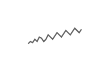
\begin{tikzpicture}[x=0.08em, y=0.08em, line width=0.4pt]
                \draw[FooterGray] (0,3) -- (1,4) -- (2,3.5) -- (3,5) -- (4,4) -- (5,6) -- (6,5.5) -- (7,4) -- (8,5) -- (9,7) -- (10,6) -- (11,5) -- (12,6.5) -- (13,8) -- (14,7) -- (15,6) -- (16,7.5) -- (17,9) -- (18,8) -- (19,7) -- (20,8.5) -- (21,10) -- (22,9) -- (23,8) -- (24,9.5);
            \end{tikzpicture}%
        }%
        \hskip0.5cm%
    }%
    \vskip6pt%
}

%=============================================================================
% PACKAGES
%=============================================================================
\usepackage[utf8]{inputenc}
\usepackage[T1]{fontenc}
\usepackage{amsmath, amssymb, amsthm}
\usepackage{mathtools}
\usepackage{bm}
\usepackage{tikz}
\usetikzlibrary{arrows.meta, positioning, shapes, calc, decorations.pathreplacing, shadings}
\usepackage{booktabs}
\usepackage{multirow}
\usepackage{array}
\usepackage{graphicx}
\usepackage{hyperref}
\usepackage{colortbl}
\usepackage{listings}
\lstset{language=Python, basicstyle=\ttfamily\scriptsize, keywordstyle=\color{MainBlue}\bfseries,
  commentstyle=\color{Forest}, stringstyle=\color{Crimson}, breaklines=true,
  frame=none, backgroundcolor=\color{VeryLightGray}, xleftmargin=2mm}
\hypersetup{colorlinks=true, linkcolor=MainBlue, urlcolor=MainBlue}
\graphicspath{{../../logos/}{../../charts/}{../../photos/}}
\hfuzz=2pt  % Suppress tiny overfull warnings (<2pt)
\vfuzz=2pt  % Suppress tiny vertical overfull warnings (<2pt)

%=============================================================================
% QUANTLET COMMAND
%=============================================================================
\newcommand{\quantlet}[2]{%
    \hfill\href{#2}{%
        \raisebox{-0.15em}{
\includegraphics[height=0.7em]{ql_logo.png}}%
        \textcolor{MainBlue}{\tiny\ #1}%
    }%
}

%=============================================================================
% CUSTOM TITLE PAGE
%=============================================================================
\defbeamertemplate*{title page}{hybrid}[1][]
{
    \vspace{0.2cm}
    % Logos row - top header (with clickable links)
    \begin{center}
        \href{https://www.ase.ro}{
\includegraphics[height=1.0cm]{ase_logo.png}}\hspace{0.3cm}%
        \href{https://theida.net}{
\includegraphics[height=1.0cm]{ida_logo.png}}\hspace{0.3cm}%
        \href{https://blockchain-research-center.com}{
\includegraphics[height=1.0cm]{brc_logo.png}}\hspace{0.3cm}%
        \href{https://www.ai4efin.ase.ro}{
\includegraphics[height=1.0cm]{ai4efin_logo.png}}\hspace{0.3cm}%
        \href{https://ipe.ro/new}{
\includegraphics[height=1.0cm]{acad_logo.png}}\hspace{0.3cm}%
        \href{https://www.digital-finance-msca.com}{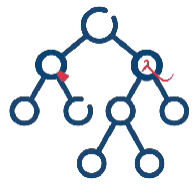
\includegraphics[height=1.0cm]{msca_logo.png}}%
    \end{center}

    \vspace{0.6cm}

    % Main title with Q logos on sides (with clickable links)
    \begin{center}
        \begin{minipage}{0.1\textwidth}
            \centering
            \href{https://quantlet.com}{
\includegraphics[height=1.1cm]{ql_logo.png}}
        \end{minipage}%
        \begin{minipage}{0.78\textwidth}
            \centering
            {\LARGE\bfseries\usebeamercolor[fg]{title}\inserttitle}

            \vspace{0.3cm}

            {\usebeamerfont{subtitle}\usebeamercolor[fg]{title}\insertsubtitle}
        \end{minipage}%
        \begin{minipage}{0.1\textwidth}
            \centering
            \href{https://quantinar.com}{
\includegraphics[height=1.1cm]{qr_logo.png}}
        \end{minipage}
    \end{center}

    \vspace{0.6cm}

    % Authors (left aligned)
    \hspace{0.5cm}{\usebeamerfont{author}\insertauthor}

    \vspace{0.3cm}

    % Institute/Affiliations (left aligned)
    \hspace{0.5cm}\begin{minipage}[t]{0.9\textwidth}
        \raggedright\small\insertinstitute
    \end{minipage}
}

%=============================================================================
% THEOREM ENVIRONMENTS
%=============================================================================
\theoremstyle{definition}
\setbeamertemplate{theorems}[numbered]
\newtheorem{defn}{Definition}
\newtheorem{thm}{Theorem}
\newtheorem{prop}{Proposition}
\newtheorem{rmk}{Remark}

%=============================================================================
% CENTRED MINIPAGE (no extra vertical space)
%=============================================================================
\newenvironment{cminipage}[1]{%
    \par\noindent\hfill\begin{minipage}{#1}\ignorespaces
}{%
    \end{minipage}\hfill\null\par
}

%=============================================================================
% CUSTOM COMMANDS
%=============================================================================
\newcommand{\E}{\mathbb{E}}
\newcommand{\Var}{\text{Var}}
\newcommand{\Cov}{\text{Cov}}
\newcommand{\Corr}{\text{Corr}}
\newcommand{\R}{\mathbb{R}}
\newcommand{\N}{\mathbb{N}}
\newcommand{\Z}{\mathbb{Z}}
\newcommand{\B}{\mathbf{B}}
\newcommand{\imark}{\textcolor{MainBlue}{\textbullet}}
\newcommand{\RMSE}{\text{RMSE}}
\newcommand{\MAE}{\text{MAE}}
\newcommand{\MAPE}{\text{MAPE}}

%=============================================================================
% TITLE INFORMATION
%=============================================================================
\title[Statistics of Financial Markets]{Statistics of Financial Markets}
\subtitle{Chapter 2: Statistical Distributions for Financial Markets}
\author[D.T. Pele]{Daniel Traian PELE}
\institute{Bucharest University of Economic Studies\\
IDA Institute Digital Assets\\
Blockchain Research Center\\
AI4EFin Artificial Intelligence for Energy Finance\\
Romanian Academy, Institute for Economic Forecasting\\
MSCA Digital Finance}
\date{}

%=============================================================================
\begin{document}
%=============================================================================

%-----------------------------------------------------------------------------
% TITLE SLIDE
%-----------------------------------------------------------------------------
{
\setbeamertemplate{headline}{}
\setbeamertemplate{footline}{}
\begin{frame}[plain]
    \titlepage
\end{frame}
}

%=============================================================================
% LEARNING OBJECTIVES
%=============================================================================
\begin{frame}{Learning Objectives}
    \begin{block}{By the end of this chapter, you will be able to:}
    \begin{enumerate}
        \item[\textcolor{MainBlue}{\textbf{1.}}] \textbf{Explain} why the choice of distribution affects financial risk estimation
        \item[\textcolor{MainBlue}{\textbf{2.}}] \textbf{Compute} log-returns and interpret their statistical properties
        \item[\textcolor{MainBlue}{\textbf{3.}}] \textbf{Identify} stylized facts of returns (heavy tails, skewness, clustering)
        \item[\textcolor{MainBlue}{\textbf{4.}}] \textbf{Compare} Normal, Student-$t$, stable, and EVT distributions
        \item[\textcolor{MainBlue}{\textbf{5.}}] \textbf{Apply} Value-at-Risk and Expected Shortfall under different distributional assumptions
        \item[\textcolor{MainBlue}{\textbf{6.}}] \textbf{Evaluate} GARCH models with non-Gaussian innovations
    \end{enumerate}
    \end{block}
\end{frame}

%=============================================================================
% TABLE OF CONTENTS
%=============================================================================
{
\setbeamertemplate{headline}{%
    \vskip10pt%
    \hbox to \paperwidth{\hskip0.5cm\hfill\hskip0.5cm}%
    \vskip4pt%
    {\color{FooterGray}\hrule height 0.4pt}%
}
\begin{frame}{}
    {\color{FooterGray}\hrule height 0.4pt}
    \vspace{0.1cm}
    {\Large\textcolor{IDAred}{\textbf{Contents}}}
    \vspace{0.2cm}
    {\small
    \begin{columns}[T]
        \begin{column}{0.48\textwidth}
            \begin{enumerate}
                \item Introduction
                \item From Prices to Log-Returns
                \item The Normal Distribution
                \item Stylized Facts
                \item The Student-$t$ Distribution
                \item Asymmetric Distributions
            \end{enumerate}
        \end{column}
        \begin{column}{0.48\textwidth}
            \begin{enumerate}\setcounter{enumi}{6}
                \item Stable Distributions
                \item Extreme Value Theory
                \item Distribution Comparison
                \item Risk Management
                \item Modern Extensions
            \end{enumerate}
        \end{column}
    \end{columns}
    }
\end{frame}
}

%#############################################################################
\section{Introduction --- Why Distributions Matter}
%#############################################################################

%--- Y3 Slide 1 ---
\begin{frame}{Why Does the Distribution Choice Matter?}
\begin{itemize}
\item If we assume the wrong distribution, we \textbf{underestimate} the probability of extreme losses
\item \textbf{Example}: October 19, 1987 --- the S\&P~500 fell 20.5\% in a single day
\begin{itemize}
\item Under the Normal assumption: a $\sim$25$\sigma$ event with probability $\approx 10^{-135}$
\item Yet it happened --- the Normal distribution is inadequate for tail events
\end{itemize}
\item Banks and regulators need to quantify ``how bad can it get?''
\item This requires \textbf{accurate distributional models}
\end{itemize}

\vspace{0.3cm}
\begin{alertblock}{Key Insight}
\begin{itemize}
\item The choice of probability distribution directly determines how much capital a bank must hold against potential losses
\end{itemize}
\end{alertblock}
\end{frame}

%--- Y3 Slide 2 ---
\begin{frame}{The Distribution Choice Problem}
\begin{itemize}
\item \textbf{Preview}: In Section~2.10 we will formally define \textbf{Value-at-Risk (VaR)}, a key risk measure that depends entirely on the distributional assumption
\item The candidates we will study:
\begin{itemize}
\item \textbf{Normal} --- the classical benchmark (thin tails)
\item \textbf{Student-$t$} --- heavier tails, finite higher moments
\item \textbf{Stable} --- heaviest tails, infinite variance possible
\item \textbf{EVT} --- models only the tails, agnostic about the center
\end{itemize}
\item Each model implies a different answer to ``how bad can it get?''
\end{itemize}

\vspace{0.2cm}
\begin{center}
\renewcommand{\arraystretch}{1.1}
\begin{tabular}{lccc}
\toprule
\textbf{Model} & \textbf{Tail Type} & \textbf{Kurtosis} & \textbf{Parameters} \\
\midrule
Normal & Exponential & 3 & 2 \\
Student-$t$ & Power law & $>3$ & 3 \\
Stable & Power law & $\infty$ & 4 \\
GPD (EVT) & Flexible & --- & 2 \\
\bottomrule
\end{tabular}
\end{center}
\end{frame}

%--- Y3 Slide 3 ---
\begin{frame}{Chapter Roadmap}
\begin{columns}[T]
\begin{column}{0.48\textwidth}
\textbf{Foundations}
\begin{enumerate}
\item From prices to log-returns
\item Normal distribution (benchmark)
\item Stylized facts of financial returns
\item Student-$t$ distribution
\item Asymmetric distributions
\end{enumerate}
\end{column}
\begin{column}{0.48\textwidth}
\textbf{Advanced Models \& Applications}
\begin{enumerate}\setcounter{enumi}{5}
\item Stable distributions
\item Extreme Value Theory
\item Distribution comparison
\item \textcolor{Crimson}{\textbf{Risk management (VaR, ES)}}
\item Modern extensions (GARCH)
\end{enumerate}
\end{column}
\end{columns}

\end{frame}

%--- MSc Slide 4 ---
\begin{frame}{Distribution Choice and Derivative Pricing}
\begin{itemize}
\item Black--Scholes assumes log-normality $\Rightarrow$ constant implied volatility
\item Empirical deviations produce the \textbf{volatility smile/skew}
\item Portfolio optimization under non-Gaussian returns: mean-variance is suboptimal
\item Regulatory context: Basel~II $\to$ Basel~III/IV framework
\begin{itemize}
\item Basel~II: 1\% VaR with Normal assumption
\item Basel~III/IV: shift from 1\% VaR to 2.5\% ES
\end{itemize}
\end{itemize}

\vspace{0.3cm}
\begin{rmk}
The entire Basel regulatory capital framework rests on distributional assumptions. Underestimating tail risk $\Rightarrow$ insufficient capital $\Rightarrow$ systemic fragility.
\end{rmk}
\end{frame}

%--- PhD Slide 5 ---
\begin{frame}{Model Uncertainty and Robust Risk Measures}
\begin{itemize}
\item \textbf{Model uncertainty}: Which distribution is ``correct''? Perhaps none.
\item \textbf{Ambiguity aversion} (Ellsberg paradox in portfolio choice)
\item Robust risk measures under distributional uncertainty:
\[
\rho_{\text{robust}}(X) = \sup_{Q \in \mathcal{Q}} \rho_Q(X)
\]
where $\mathcal{Q}$ is an ambiguity set of plausible distributions
\item Minimax approaches: worst-case distributional analysis
\item \textbf{Model risk quantification}: range of VaR/ES across plausible models provides a ``model risk premium''
\end{itemize}
\end{frame}

%#############################################################################
\section{From Prices to Log-Returns}
%#############################################################################

%--- Y3 Slide 1 ---
\begin{frame}{Definition of Log-Returns}
\begin{defn}[Log-Return]
The \textbf{log-return} (continuously compounded return) at time $t$ is:
\[
r_t = \ln\!\left(\frac{P_t}{P_{t-1}}\right) = \ln P_t - \ln P_{t-1}
\]
where $P_t$ is the asset price at time $t$.
\end{defn}

\vspace{0.2cm}
\begin{itemize}
\item \textbf{Additivity}: Multi-period returns are sums: $r_{t:t+k} = \sum_{i=1}^{k} r_{t+i}$
\item \textbf{Approximation}: For small returns, $r_t \approx (P_t - P_{t-1})/P_{t-1}$
\item \textbf{Statistical motivation}: Additive structure enables standard probability theory (CLT, stable limits)
\end{itemize}
\end{frame}

%--- Y3 Slide 2 ---
\begin{frame}{Properties of Log-Returns}
\begin{columns}[T]
\begin{column}{0.48\textwidth}
\textbf{Why log-returns?}
\begin{itemize}
\item Time-additive: $r_{[0,T]} = \sum_{t=1}^{T} r_t$
\item Symmetric: $+5\%$ and $-5\%$ are comparable
\item Unbounded below: can model large losses
\item Enable CLT-based inference
\end{itemize}
\end{column}
\begin{column}{0.48\textwidth}
\textbf{Simple vs.\ log-returns}
\begin{itemize}
\item Simple return: $R_t = \frac{P_t - P_{t-1}}{P_{t-1}}$
\item Relationship: $r_t = \ln(1 + R_t)$
\item Simple returns are \textit{not} additive across time
\item But simple returns \textit{are} additive across portfolio assets
\end{itemize}
\end{column}
\end{columns}

\vspace{0.3cm}
\begin{exampleblock}{Convention}
\begin{itemize}
\item Throughout this chapter, $r_t$ denotes the \textbf{log-return} unless stated otherwise
\end{itemize}
\end{exampleblock}
\end{frame}

%--- MSc Slide 3 ---
\begin{frame}{Continuous-Time Limit}
\begin{itemize}
\item Geometric Brownian Motion: $dS/S = \mu\,dt + \sigma\,dW$
\item By It\^{o}'s lemma: $d\ln S = (\mu - \sigma^2/2)\,dt + \sigma\,dW$
\item Jensen's inequality: $\E[\ln(P_T/P_0)] \neq \ln(\E[P_T/P_0])$
\begin{itemize}
\item The arithmetic mean return exceeds the geometric mean return
\item Difference $\approx \sigma^2/2$ (``volatility drag'')
\end{itemize}
\item Log-return vs.\ simple return: implications for portfolio aggregation
\begin{itemize}
\item Log-returns: additive across \textit{time}
\item Simple returns: additive across \textit{assets}
\item Neither is additive in both dimensions simultaneously
\end{itemize}
\end{itemize}
\end{frame}

%--- PhD Slide 4 ---
\begin{frame}{Semimartingale Representation}
\begin{itemize}
\item Price processes modeled as \textbf{semimartingales}: $S_t = S_0 + A_t + M_t$
\item It\^{o}'s lemma for semimartingales with jumps:
\[
d\ln S_t = \frac{dS_t}{S_{t^-}} - \frac{1}{2}\frac{d[S,S]_t^c}{S_{t^-}^2} + \sum_{s \leq t}\left(\ln\frac{S_s}{S_{s^-}} - \frac{\Delta S_s}{S_{s^-}}\right)
\]
\item Quadratic variation and realized volatility:
\[
[X,X]_t = \lim_{\|\Pi\| \to 0} \sum_{i} (X_{t_{i+1}} - X_{t_i})^2
\]
\item Non-continuous price processes: jumps and L\'{e}vy--It\^{o} decomposition
\item High-frequency returns reveal microstructure noise, bid-ask bounce, Epps effect
\end{itemize}
\end{frame}

%#############################################################################
\section{The Normal Distribution}
%#############################################################################

%--- Y3 Slide 1 ---
\begin{frame}{The Normal Distribution --- Definition and Properties}
\begin{defn}[Normal Distribution]
$X \sim N(\mu, \sigma^2)$ if:
\[
f(x) = \frac{1}{\sigma\sqrt{2\pi}}\exp\!\left(-\frac{(x-\mu)^2}{2\sigma^2}\right), \quad x \in \R.
\]
\end{defn}

\begin{columns}[T]
\begin{column}{0.48\textwidth}
\textbf{Moments}:
\begin{itemize}
\item $\E[X] = \mu$, \quad $\Var(X) = \sigma^2$
\item Skewness $= 0$
\item Kurtosis $= 3$ (excess kurtosis $= 0$)
\end{itemize}
\end{column}
\begin{column}{0.48\textwidth}
\textbf{Key properties}:
\begin{itemize}
\item Symmetric about $\mu$
\item 68--95--99.7 rule
\item Tails decay as $e^{-x^2/2}$
\end{itemize}
\end{column}
\end{columns}
\end{frame}

%--- Y3 Slide 2 ---
\begin{frame}{Quantiles and the Central Limit Theorem}
\begin{itemize}
\item \textbf{Quantiles}: The $\alpha$-quantile of $N(\mu, \sigma^2)$ is:
\[
q_\alpha = \mu + \sigma\,\Phi^{-1}(\alpha)
\]
This will be used in Section~2.10 to define Value-at-Risk
\item \textbf{Key quantiles}: $\Phi^{-1}(0.01) = -2.326$, \quad $\Phi^{-1}(0.05) = -1.645$
\end{itemize}

\vspace{0.2cm}
\begin{thm}[Central Limit Theorem]
If $X_1, X_2, \ldots$ are i.i.d.\ with $\E[X_i] = \mu$ and $\Var(X_i) = \sigma^2 < \infty$, then:
\[
\frac{\bar{X}_n - \mu}{\sigma/\sqrt{n}} \xrightarrow{d} N(0,1).
\]
\end{thm}

\begin{itemize}
\item \textbf{Stability}: Sum of independent normals is normal: $X + Y \sim N(\mu_1+\mu_2, \sigma_1^2+\sigma_2^2)$
\end{itemize}
\end{frame}

%--- Y3 Slide 3 ---
\begin{frame}{CLT Illustration}
\begin{center}
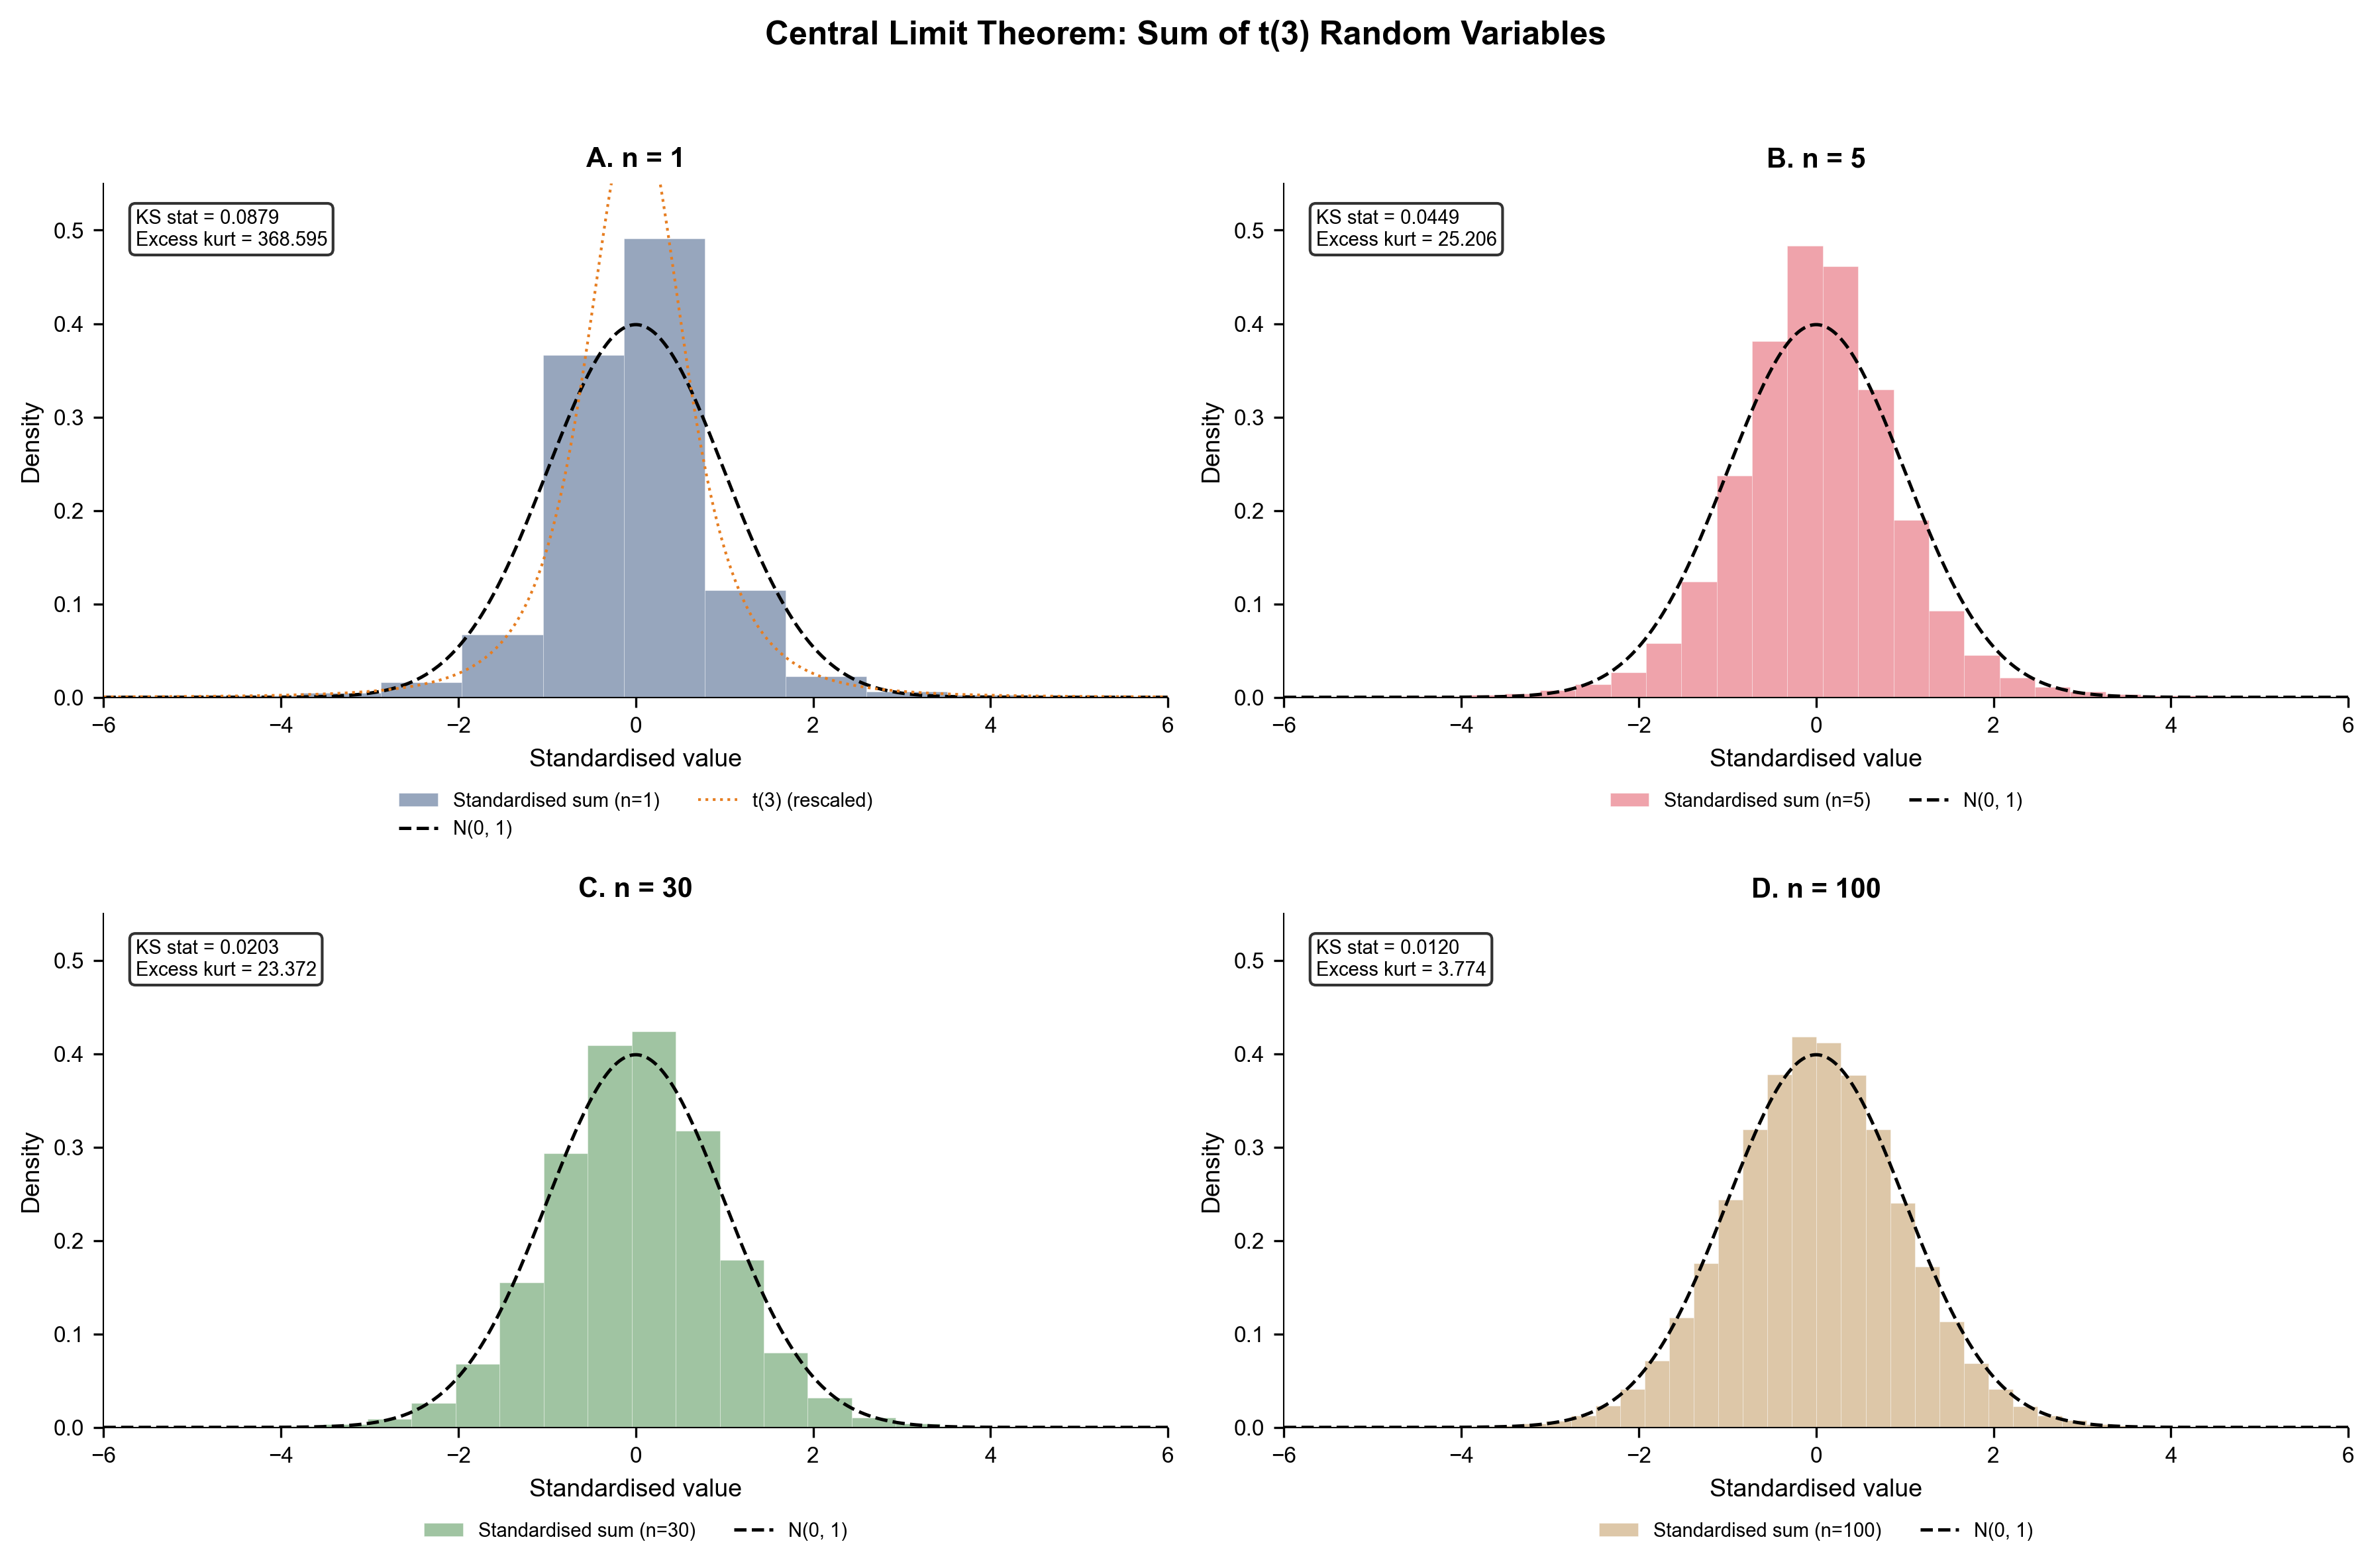
\includegraphics[width=0.55\textwidth]{ch2_clt_illustration.png}
\end{center}
\begin{itemize}
\item As $n$ increases, $\bar{X}_n$ approaches normality
\item \textbf{Limitation}: CLT requires finite variance --- what if $\sigma^2 = \infty$?
\end{itemize}
\end{frame}

%--- Y3 Slide 4 ---
\begin{frame}{Normal Fit to S\&P 500 Returns}
\quantlet{SFM\_ch2\_normal\_test}{https://github.com/QuantLet/SFM/tree/master/QID-3447-SFMnorm}
\begin{center}
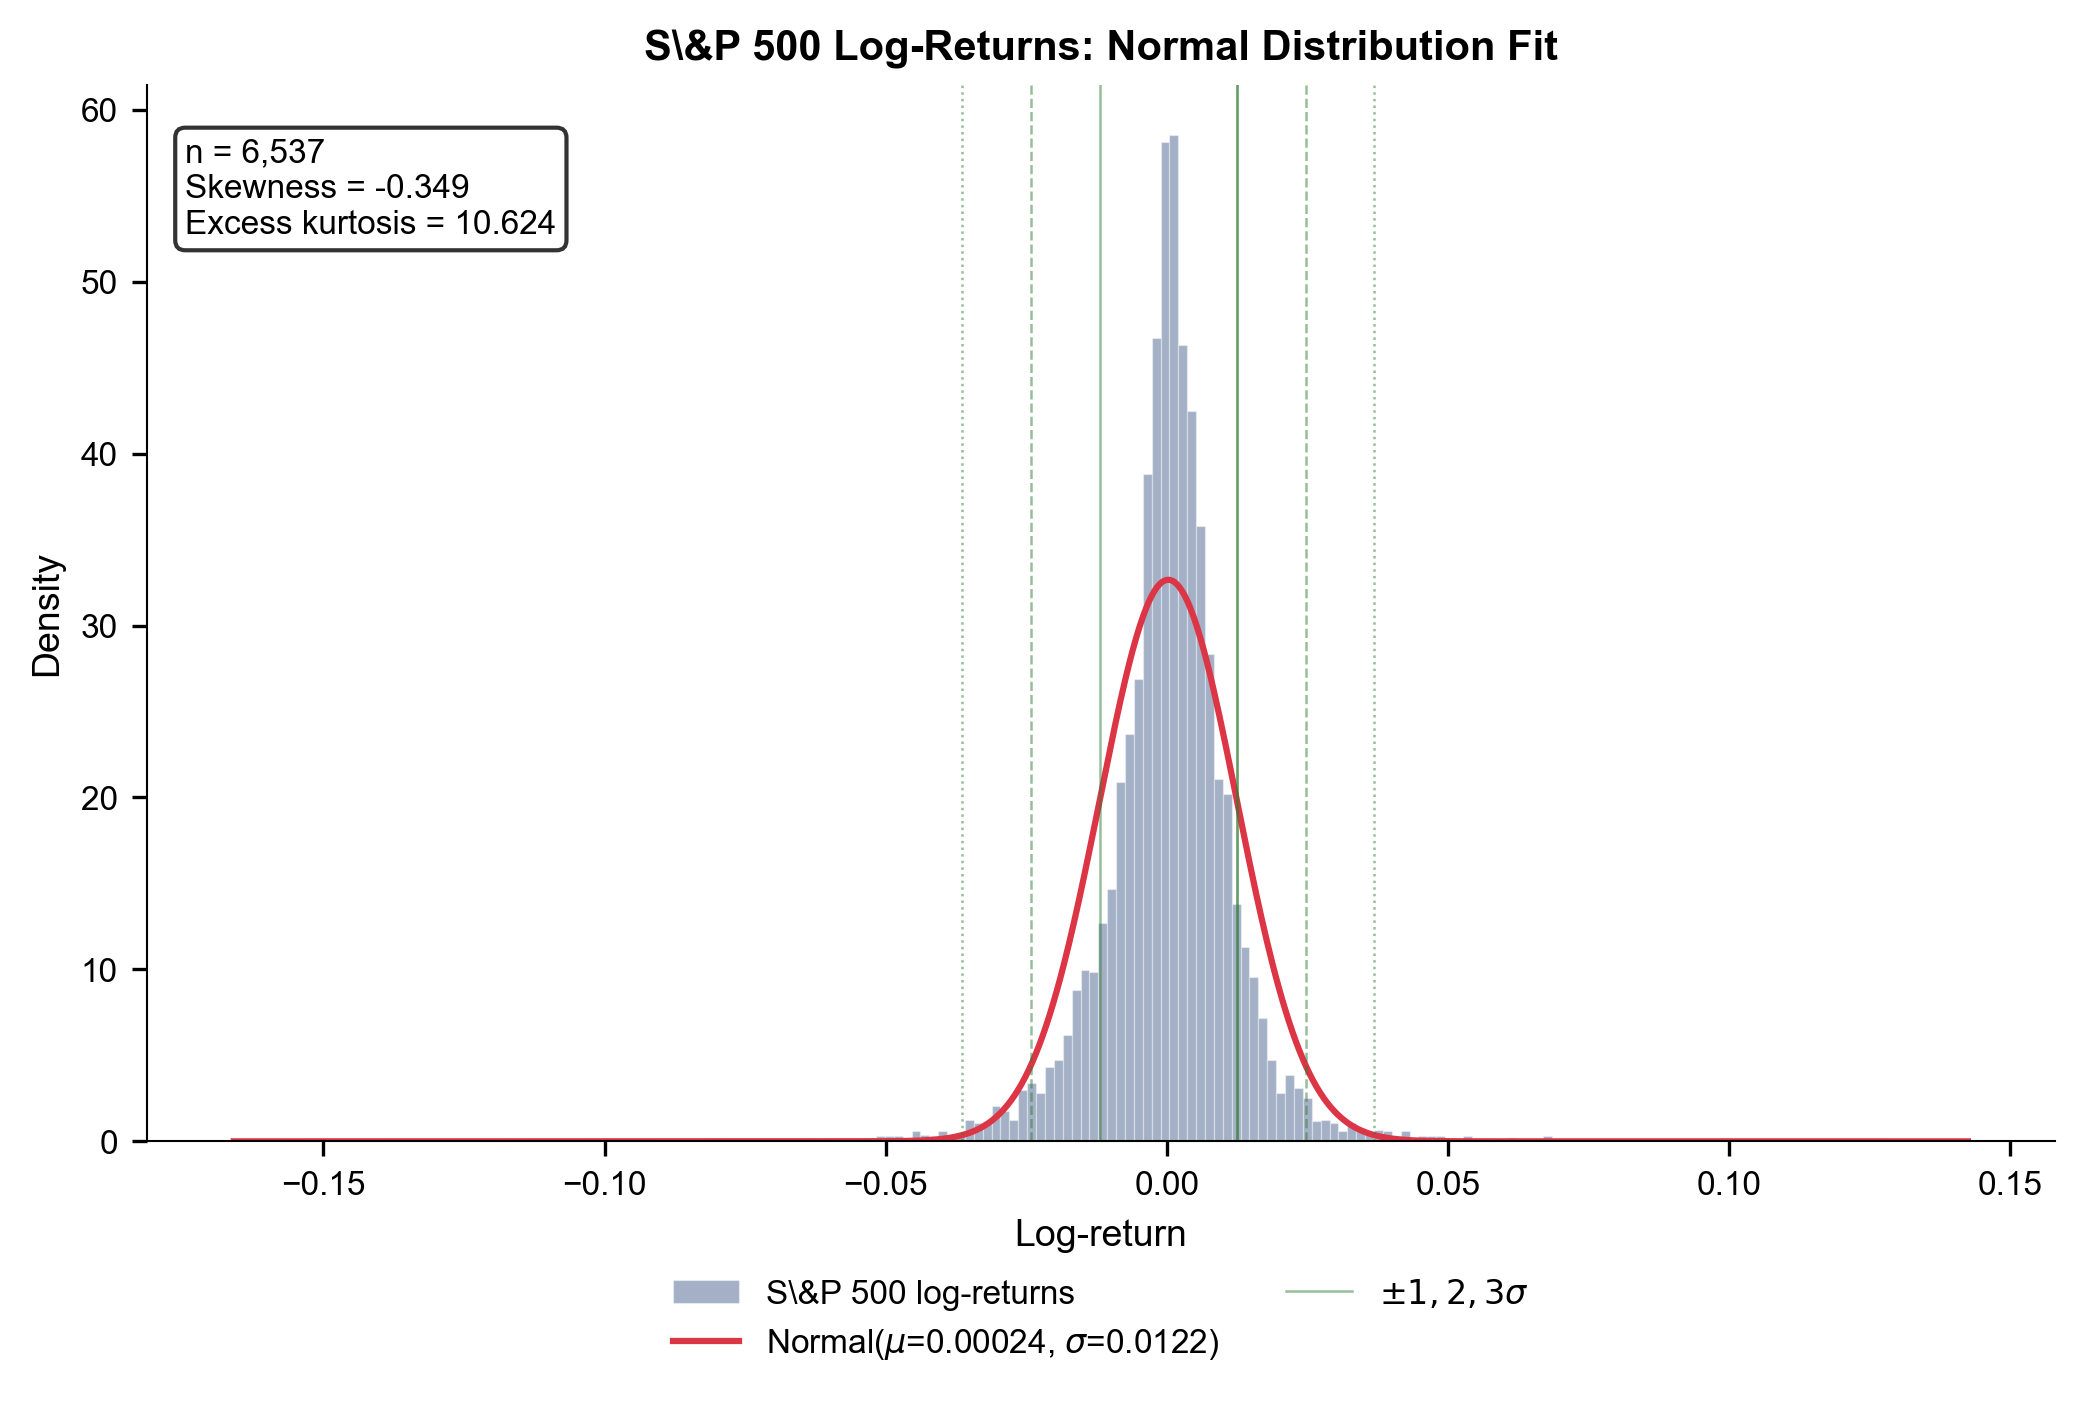
\includegraphics[width=0.5\textwidth]{ch2_normal_fit.png}
\end{center}
\begin{itemize}
\item Normal PDF fits the center well but \textbf{misses the tails}
\item Histogram has more mass in the tails than Normal predicts
\end{itemize}
\end{frame}

%--- MSc Slide 5 ---
\begin{frame}{Maximum Entropy and Normality Tests}
\begin{itemize}
\item \textbf{Maximum entropy}: Among all distributions with given $(\mu, \sigma^2)$, the Normal maximizes Shannon entropy $H = -\int f\ln f\,dx$
\item \textbf{Normality tests}:
\end{itemize}

\vspace{0.1cm}
\begin{columns}[T]
\begin{column}{0.48\textwidth}
\textbf{Jarque--Bera test}:
\[
JB = \frac{n}{6}\!\left(S^2 + \frac{(K-3)^2}{4}\right) \sim \chi^2(2)
\]
Tests skewness $S$ and excess kurtosis $K-3$ jointly.
\end{column}
\begin{column}{0.48\textwidth}
\textbf{Other tests}:
\begin{itemize}
\item Shapiro--Wilk (regression-based)
\item Anderson--Darling (CDF, tail-weighted)
\item Kolmogorov--Smirnov (sup CDF distance)
\end{itemize}
\end{column}
\end{columns}

\vspace{-0.2cm}
\begin{center}
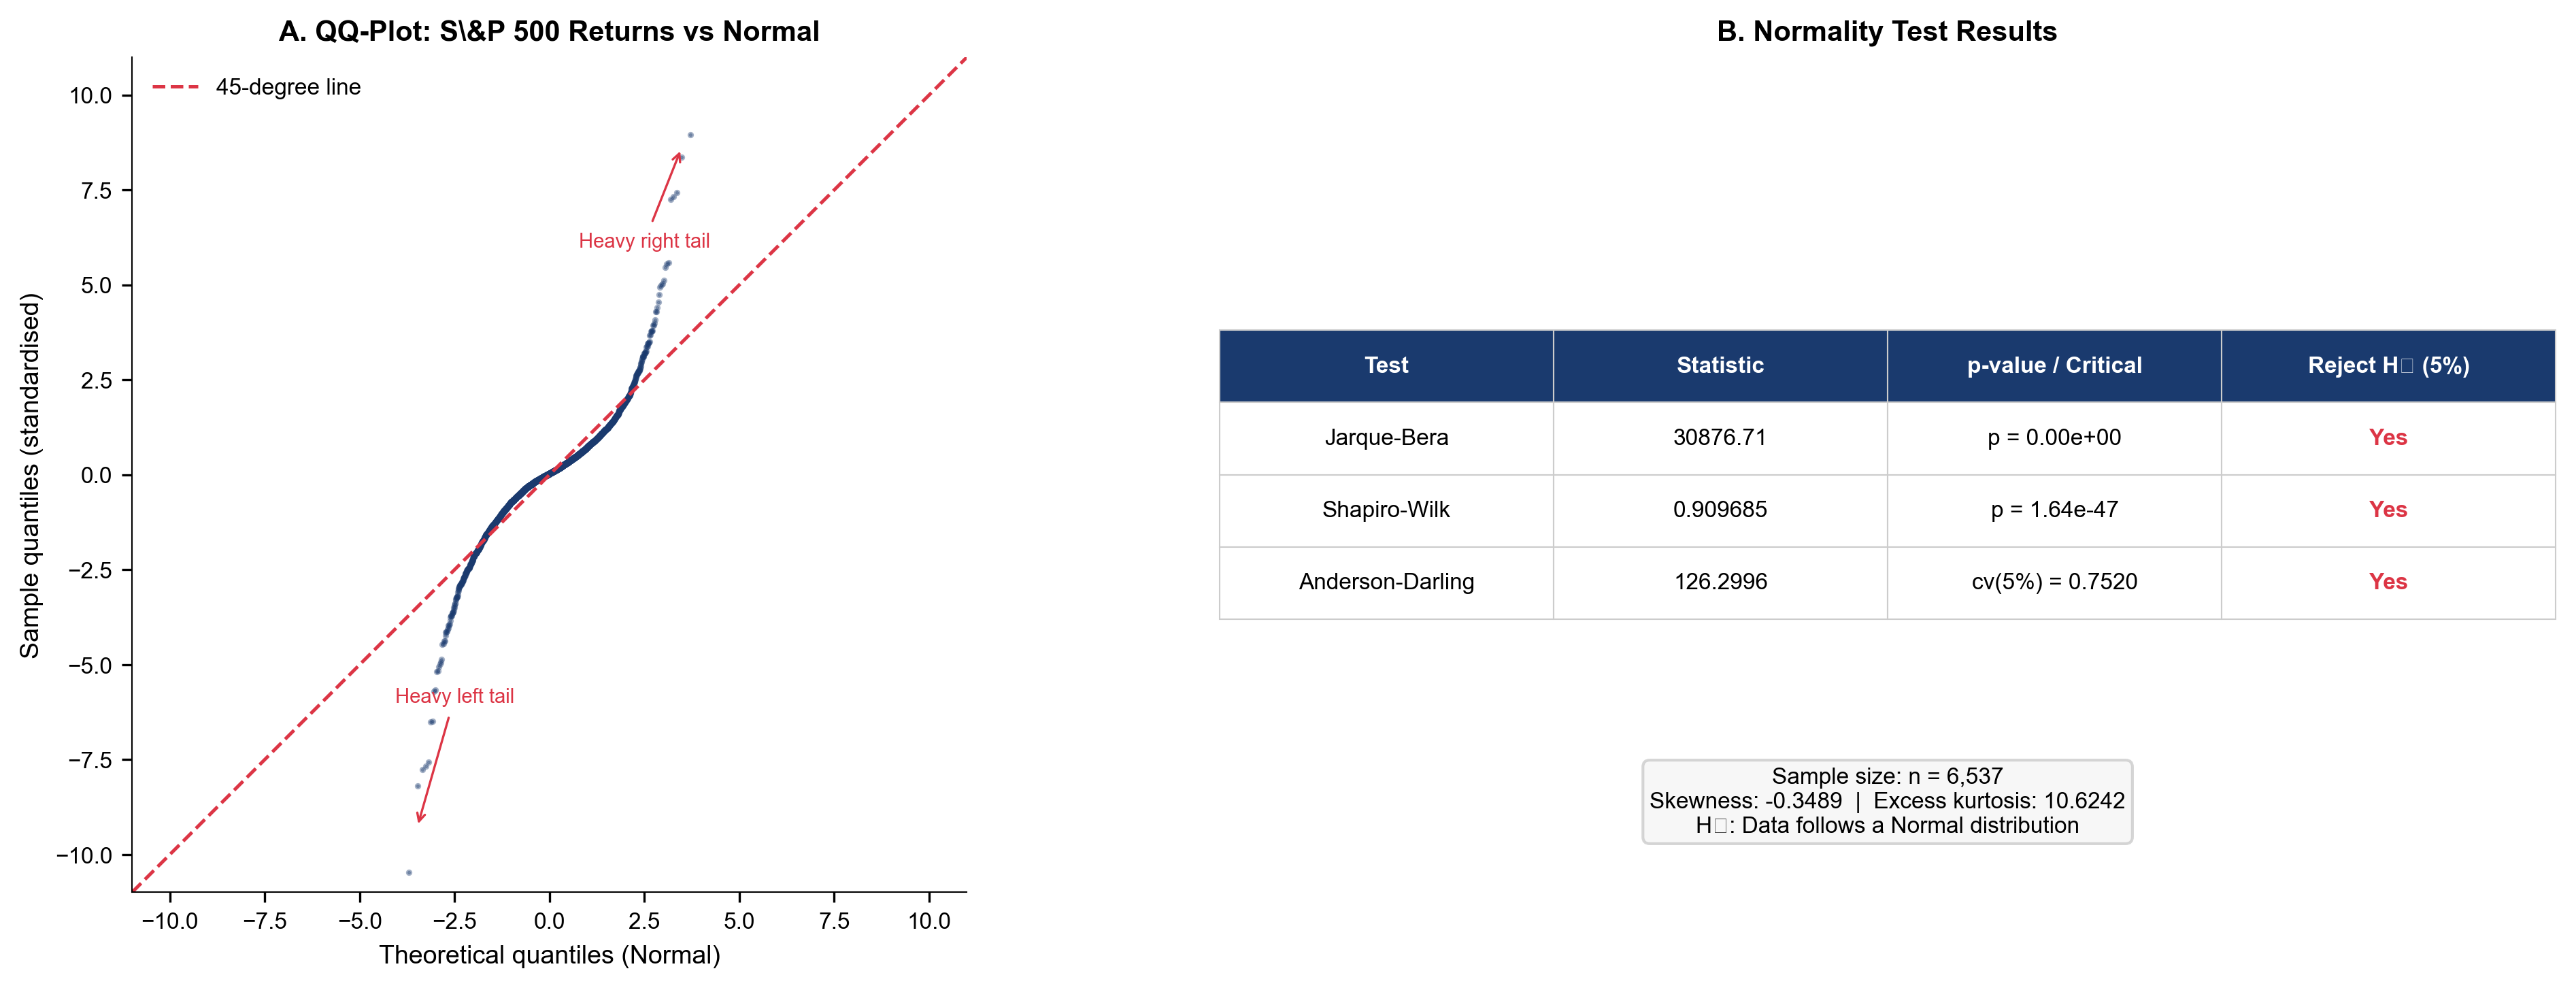
\includegraphics[height=0.30\textheight]{ch2_normality_tests.png}
\end{center}
\end{frame}

%--- MSc Slide 6 ---
\begin{frame}{Normality Tests --- Empirical Results}
\begin{itemize}
\item Moment generating function: $M_X(t) = \exp(\mu t + \sigma^2 t^2/2)$
\item Multivariate normal: $\bm{X} \sim N(\bm{\mu}, \bm{\Sigma})$ with Mahalanobis distance
\end{itemize}

\vspace{0.1cm}
\begin{center}
\renewcommand{\arraystretch}{1.0}
\begin{tabular}{lccl}
\toprule
\textbf{Test} & \textbf{Statistic} & \textbf{$p$-value} & \textbf{Decision} \\
\midrule
Jarque--Bera & $>1000$ & $<0.001$ & Reject $H_0$ \\
Shapiro--Wilk & $<0.99$ & $<0.001$ & Reject $H_0$ \\
Anderson--Darling & $>10$ & $<0.001$ & Reject $H_0$ \\
\bottomrule
\end{tabular}
\end{center}

\begin{alertblock}{Conclusion}
\begin{itemize}
\item Normality is overwhelmingly rejected for daily financial returns
\item The Normal distribution underestimates tail risk
\end{itemize}
\end{alertblock}
\end{frame}

%--- PhD Slide 7 ---
\begin{frame}{Berry--Esseen Bounds and Convergence Rates}
\begin{thm}[Berry--Esseen]
If $X_1, X_2, \ldots$ are i.i.d.\ with $\E[X_i]=0$, $\E[X_i^2]=\sigma^2$, $\E[|X_i|^3]=\rho < \infty$, then:
\[
\sup_x \left|F_n(x) - \Phi(x)\right| \leq \frac{C\,\rho}{\sigma^3\sqrt{n}}
\]
where $C \leq 0.4748$ (Shevtsova, 2011).
\end{thm}

\begin{itemize}
\item Rate of convergence: $O(n^{-1/2})$ --- slow for heavy-tailed data
\item Edgeworth expansions refine the CLT approximation for finite $n$
\item \textbf{Normal as stable}: $N(\mu,\sigma^2) = S(2, 0, \sigma/\sqrt{2}, \mu)$ --- the $\alpha=2$ member of the stable family
\item When $\E[X_i^2] = \infty$: CLT fails, but the \textbf{Generalized CLT} gives stable limits
\end{itemize}
\end{frame}

%#############################################################################
\section{Stylized Facts of Financial Returns}
%#############################################################################

%--- Y3 Slide 1 ---
\begin{frame}{Fat Tails and Excess Kurtosis}
\begin{itemize}
\item \textbf{Kurtosis}: $\kappa = \E[(X-\mu)^4]/\sigma^4$; \quad excess kurtosis: $\kappa_e = \kappa - 3$
\item Normal distribution: $\kappa_e = 0$
\item Typical daily equity kurtosis: $\kappa \in [5, 50]$, so $\kappa_e \gg 0$
\item \textbf{Interpretation}: Extreme returns occur far more often than the Normal predicts
\end{itemize}

\vspace{0.2cm}
\begin{center}
\renewcommand{\arraystretch}{1.1}
\begin{tabular}{lcc}
\toprule
\textbf{Asset} & \textbf{Skewness} & \textbf{Excess Kurtosis} \\
\midrule
S\&P 500 (daily) & $-0.3$ & $\approx 10$ \\
FTSE 100 (daily) & $-0.2$ & $\approx 8$ \\
USD/EUR (daily) & $-0.1$ & $\approx 5$ \\
Bitcoin (daily) & $-0.5$ & $\approx 15$ \\
\bottomrule
\end{tabular}
\end{center}
\end{frame}

%--- Y3 Slide 2 ---
\begin{frame}{Negative Skewness and Volatility Clustering}
\begin{columns}[T]
\begin{column}{0.48\textwidth}
\textbf{Negative skewness}
\begin{itemize}
\item Left tail heavier than right tail
\item Especially pronounced for equity indices
\item Crashes are sharper than rallies
\item Skewness $S = \E[(X-\mu)^3]/\sigma^3 < 0$
\end{itemize}
\end{column}
\begin{column}{0.48\textwidth}
\textbf{Volatility clustering}
\begin{itemize}
\item ``Large changes followed by large changes'' (Mandelbrot, 1963)
\item $\Corr(|r_t|, |r_{t+k}|) > 0$ for large $k$
\item Returns are uncorrelated but \textbf{not independent}
\item $\Corr(r_t, r_{t+k}) \approx 0$ but $\Corr(r_t^2, r_{t+k}^2) > 0$
\end{itemize}
\end{column}
\end{columns}

\vspace{0.3cm}
\begin{block}{Implication}
\begin{itemize}
\item A single i.i.d.\ distribution cannot capture volatility clustering
\item We need time-varying models (GARCH, Section~2.11)
\end{itemize}
\end{block}
\end{frame}

%--- Y3 Slide 3 ---
\begin{frame}{Aggregational Gaussianity}
\begin{itemize}
\item \textbf{Key observation}: As the holding period increases, the distribution of returns becomes \textit{more Gaussian}
\item Daily returns: high kurtosis, heavy tails
\item Weekly returns: moderate kurtosis
\item Monthly returns: closer to Normal
\item \textbf{Mechanism}: CLT-like effect --- monthly return $= \sum$ of $\sim$22 daily returns
\end{itemize}

\vspace{0.2cm}
\begin{center}
\renewcommand{\arraystretch}{1.1}
\begin{tabular}{lcc}
\toprule
\textbf{Frequency} & \textbf{Excess Kurtosis} & \textbf{JB $p$-value} \\
\midrule
Daily & $\approx 10$ & $< 0.001$ \\
Weekly & $\approx 4$ & $< 0.001$ \\
Monthly & $\approx 1.5$ & $\approx 0.05$ \\
Quarterly & $\approx 0.5$ & $\approx 0.3$ \\
\bottomrule
\end{tabular}
\end{center}
\end{frame}

%--- Y3 Slide 4 ---
\begin{frame}{Summary of Stylized Facts}
\begin{enumerate}
\item \textbf{Fat tails}: $\kappa_e \gg 0$ --- extreme events more frequent than Normal
\item \textbf{Negative skewness}: Left tail heavier (equities)
\item \textbf{Volatility clustering}: Periods of high/low volatility persist
\item \textbf{Aggregational Gaussianity}: Kurtosis decreases with horizon
\item \textbf{No return autocorrelation}: $\Corr(r_t, r_{t+k}) \approx 0$ for $k \geq 1$
\item \textbf{Squared return autocorrelation}: $\Corr(r_t^2, r_{t+k}^2) > 0$
\end{enumerate}

\vspace{0.3cm}
\begin{alertblock}{The Challenge}
\begin{itemize}
\item Any adequate model for financial returns must reproduce these stylized facts
\item The Normal distribution fails on points 1, 2, and 3
\end{itemize}
\end{alertblock}
\end{frame}

%--- MSc Slide 5 ---
\begin{frame}{Leverage Effect and Long Memory}
\begin{columns}[T]
\begin{column}{0.48\textwidth}
\textbf{Leverage effect}
\begin{itemize}
\item Negative returns increase future volatility \textit{more} than positive returns of equal magnitude
\item Asymmetric response: $\Corr(r_t, \sigma_{t+1}^2) < 0$
\item Named after Black (1976): falling stock price $\Rightarrow$ higher leverage $\Rightarrow$ higher risk
\item Captured by GJR-GARCH, EGARCH
\end{itemize}
\end{column}
\begin{column}{0.48\textwidth}
\textbf{Long memory in volatility}
\begin{itemize}
\item $\Corr(|r_t|, |r_{t+k}|)$ decays \textit{slowly} (hyperbolically, not exponentially)
\item Hurst exponent $H > 0.5$ for $|r_t|$
\item Standard GARCH: exponential decay
\item FIGARCH, HAR models capture long memory
\end{itemize}
\end{column}
\end{columns}
\end{frame}

%--- MSc Slide 6 ---
\begin{frame}{Gain/Loss Asymmetry}
\begin{itemize}
\item \textbf{Gain/loss asymmetry}: Stock prices decline faster than they rise
\item Large drawdowns happen in days; recovery takes months or years
\item This asymmetry is distinct from skewness --- it concerns the \textit{dynamics}, not the marginal distribution
\item \textbf{Absence of return autocorrelation}: $\Corr(r_t, r_{t+k}) \approx 0$ for $k \geq 1$
\begin{itemize}
\item Markets are approximately efficient at the mean level
\item But dependence exists in higher moments ($r_t^2$, $|r_t|$)
\end{itemize}
\end{itemize}
\end{frame}

%--- PhD Slide 7 ---
\begin{frame}{Cont (2001) Taxonomy and Multifractal Models}
\begin{itemize}
\item Cont (2001): systematic taxonomy of 11 stylized facts for asset returns
\item \textbf{Multifractal models} (Mandelbrot, Fisher \& Calvet, 1997):
\begin{itemize}
\item $\E[|r_t|^q] \propto \Delta t^{\zeta(q)}$ with \textit{nonlinear} $\zeta(q)$ (multiscaling)
\item Unifractal: $\zeta(q) = qH$ (linear); multifractal: $\zeta(q)$ concave
\end{itemize}
\item Cross-correlation structure and multivariate stylized facts
\item Intraday stylized facts: microstructure noise, bid-ask bounce, Epps effect
\end{itemize}
\end{frame}

%--- PhD Slide 8 ---
\begin{frame}{Fractal Structure and Power Laws}
\begin{itemize}
\item \textbf{Power-law tails}: $P(|r| > x) \sim x^{-\alpha}$ with $\alpha \in [2, 5]$ for most financial assets
\item Tail exponent $\alpha$ is remarkably stable across assets and time periods
\item \textbf{Self-similarity}: Return distributions at different time scales are related by scaling
\item Connection to stable distributions: if $\alpha < 2$, the GCLT implies stable limits
\item The ``inverse cubic law'' (Gopikrishnan et al., 1999): $\alpha \approx 3$ for US equities
\item Debate: true power law vs.\ slowly varying tails
\end{itemize}
\end{frame}

%#############################################################################
\section{The Student-$t$ Distribution}
%#############################################################################

%--- Y3 Slide 1 ---
\begin{frame}{Student-$t$ Distribution --- Definition}
\begin{defn}[Student-$t$ Distribution]
$X \sim t_\nu$ if:
\[
f(x;\nu) = \frac{\Gamma\!\left(\frac{\nu+1}{2}\right)}{\sqrt{\nu\pi}\,\Gamma\!\left(\frac{\nu}{2}\right)} \left(1 + \frac{x^2}{\nu}\right)^{-(\nu+1)/2}, \quad x \in \R.
\]
\end{defn}

\begin{itemize}
\item Single parameter $\nu > 0$ (\textbf{degrees of freedom}) controls tail heaviness
\item $\E[X] = 0$ ($\nu > 1$); \quad $\Var(X) = \frac{\nu}{\nu-2}$ ($\nu > 2$)
\item Excess kurtosis: $\kappa_e = \frac{6}{\nu-4}$ ($\nu > 4$)
\item $\nu \to \infty$: converges to $N(0,1)$; \quad $\nu = 1$: Cauchy distribution
\item Tails: $f(x) \sim |x|^{-(\nu+1)}$ \textbf{(power law)}
\end{itemize}
\end{frame}

%--- Y3 Slide 2 ---
\begin{frame}{Student-$t$ PDFs --- Effect of $\nu$}
\quantlet{SFM\_ch2\_student\_t\_fit}{https://github.com/QuantLet/SFM/tree/master/QID-3447-SFMstudent}

\begin{center}
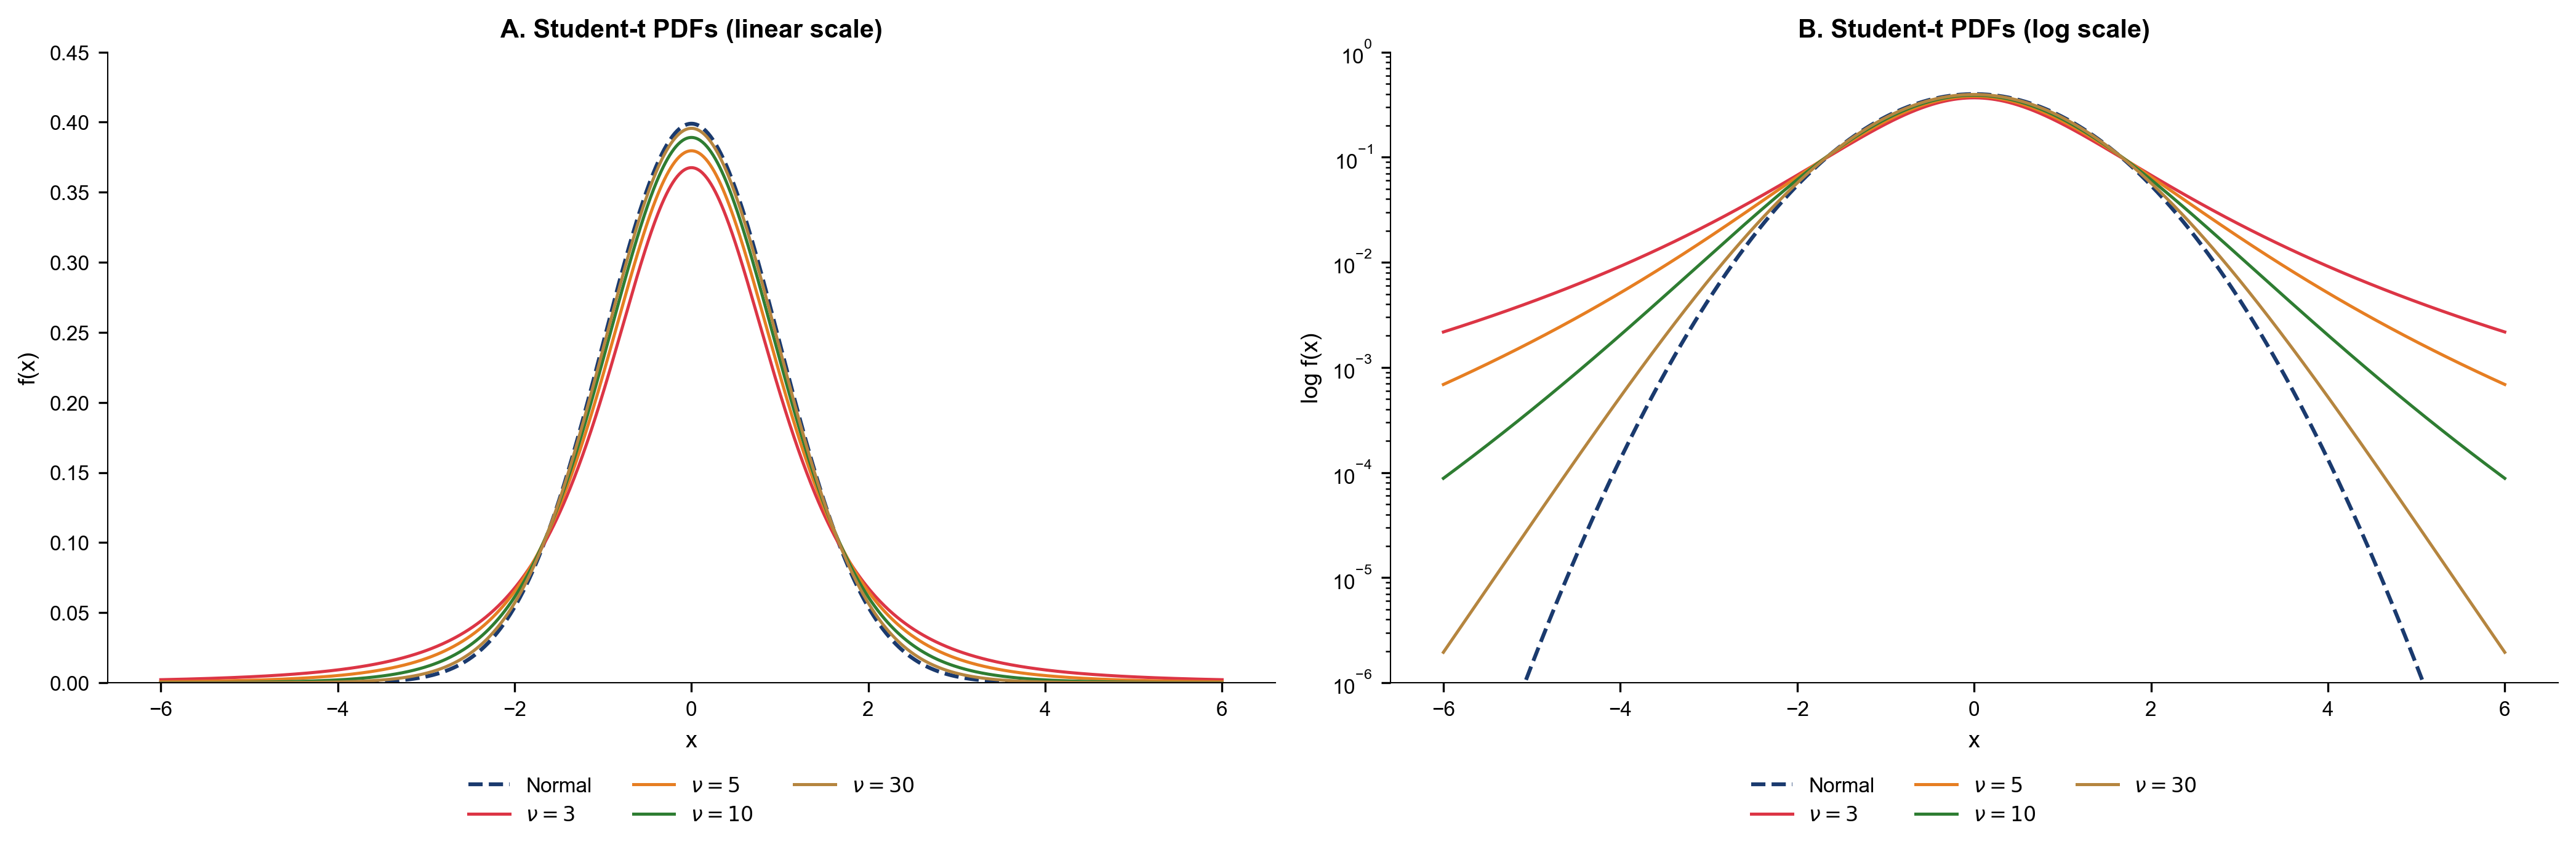
\includegraphics[width=0.72\textwidth]{ch2_student_t_pdfs.png}
\end{center}

\begin{itemize}
\item Smaller $\nu$ $\Rightarrow$ heavier tails, higher peak
\item Financial returns: typically $\hat{\nu} \in [3, 8]$ for daily equity data
\end{itemize}
\end{frame}

%--- Y3 Slide 3 ---
\begin{frame}{Student-$t$ Fit to S\&P 500}
\begin{center}
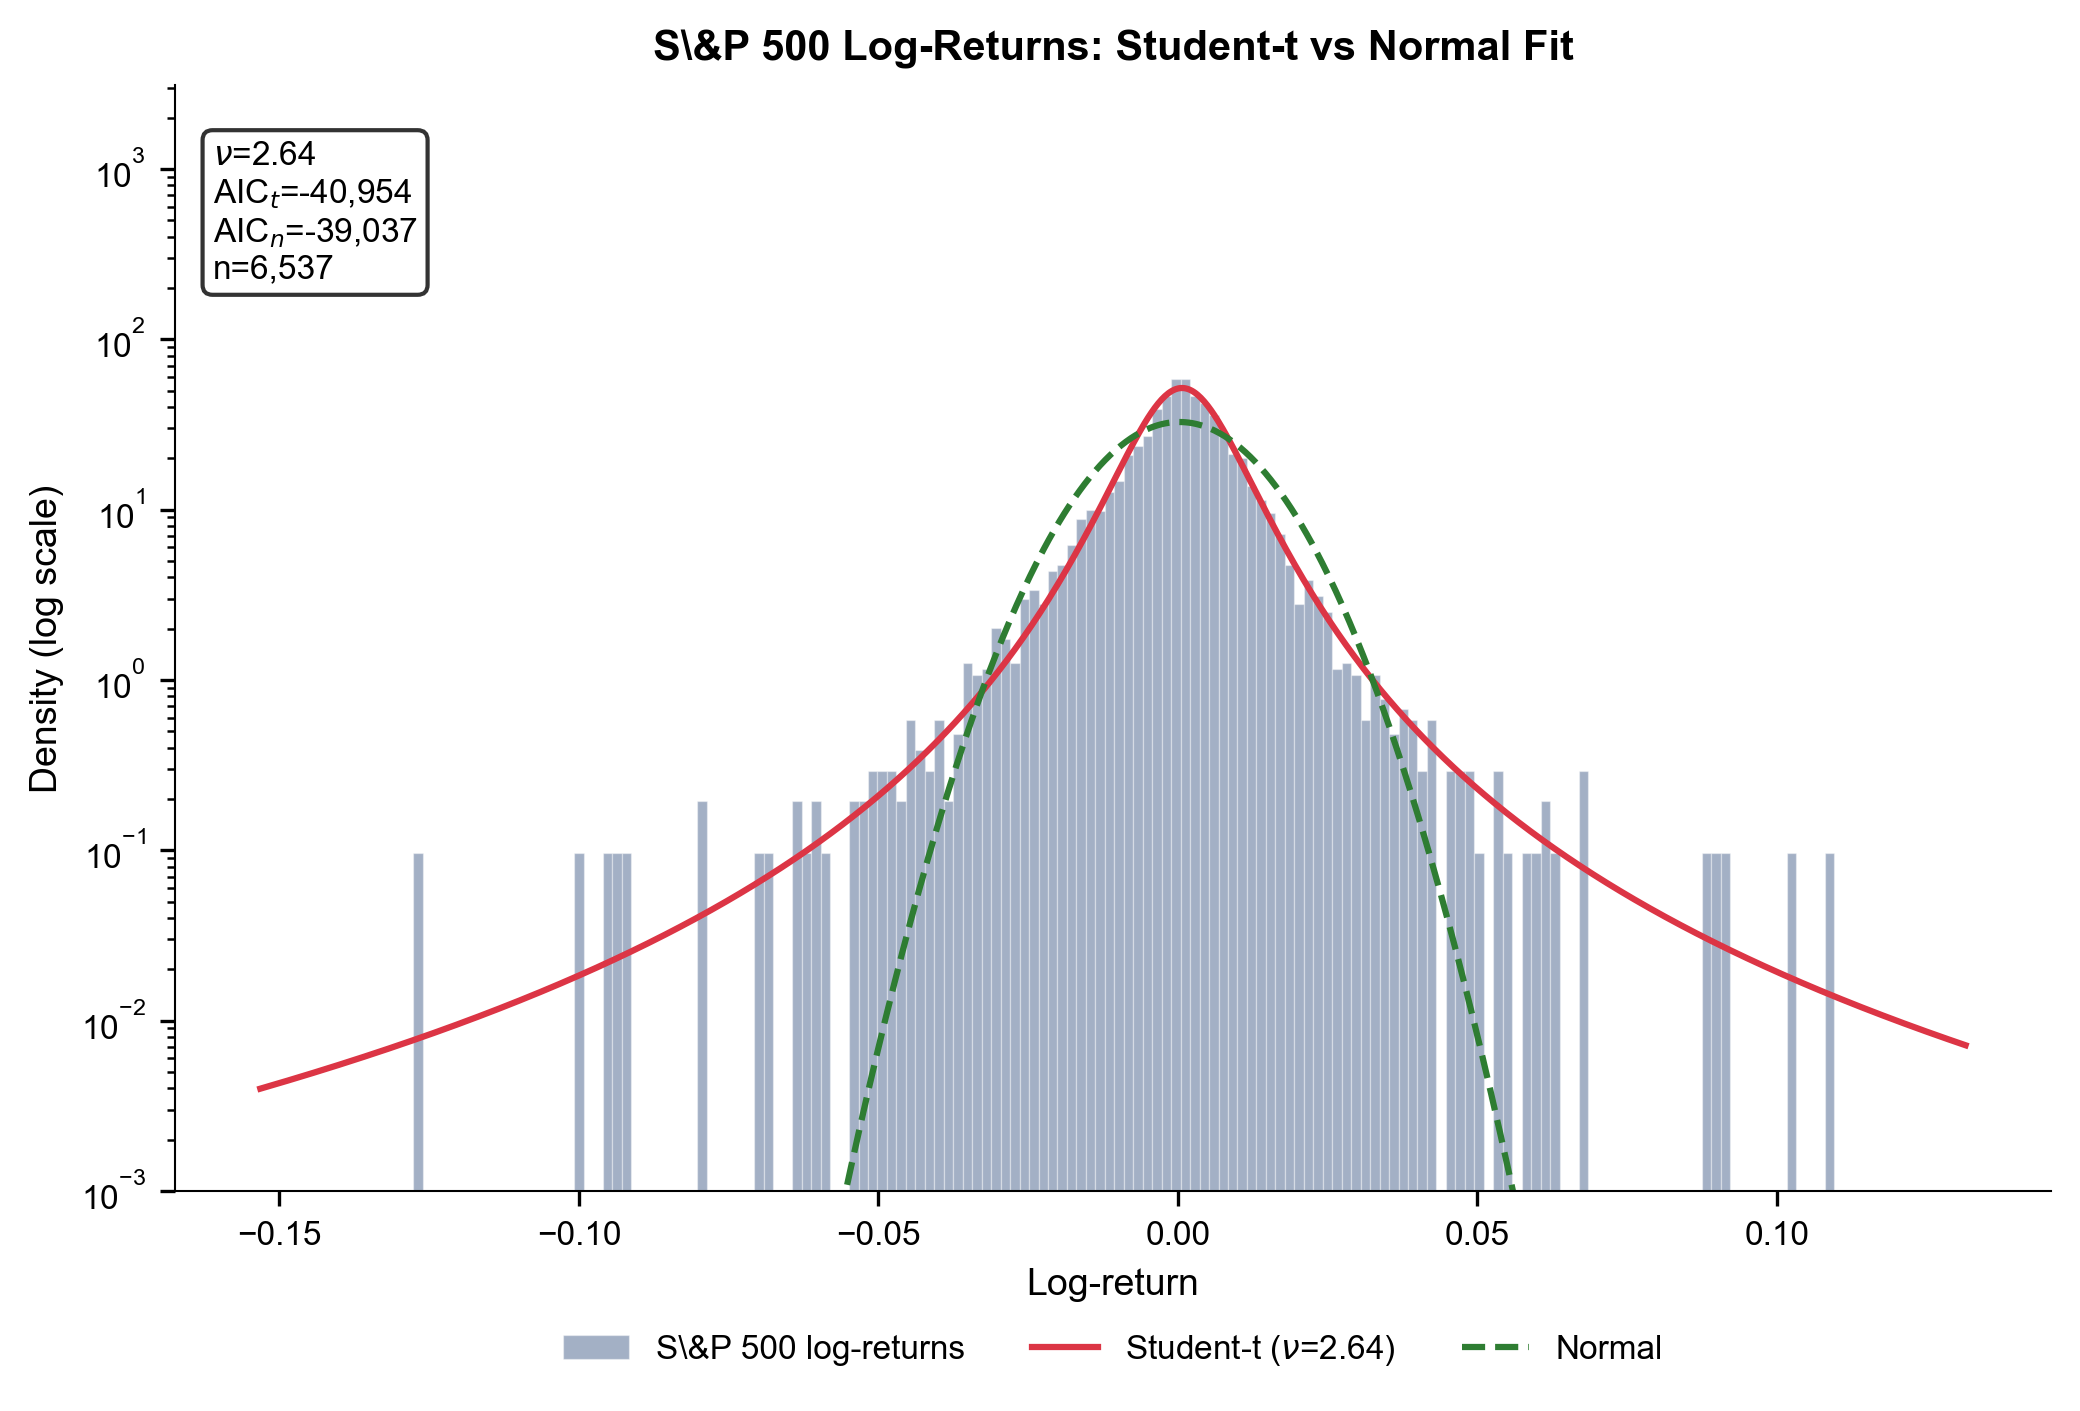
\includegraphics[width=0.55\textwidth]{ch2_student_t_fit.png}
\end{center}
\begin{itemize}
\item Student-$t$ captures the heavy tails much better than the Normal
\item Estimated $\hat{\nu} \approx 4$--$5$ for daily S\&P~500; center and tails well-matched
\end{itemize}
\end{frame}

%--- Y3 Slide 4 ---
\begin{frame}{Why Student-$t$ for Finance?}
\begin{center}
\renewcommand{\arraystretch}{1.2}
\begin{tabular}{lcc}
\toprule
\textbf{Property} & \textbf{Normal} & \textbf{Student-$t$} \\
\midrule
Tail decay & Exponential ($e^{-x^2/2}$) & Power law ($|x|^{-\nu-1}$) \\
Excess kurtosis & 0 & $6/(\nu-4)$ \\
Parameters & 2 ($\mu, \sigma$) & 3 ($\mu, \sigma, \nu$) \\
Extreme events & Very rare & More frequent \\
Limit & --- & Normal ($\nu \to \infty$) \\
\bottomrule
\end{tabular}
\end{center}

\vspace{0.3cm}
\begin{block}{Key Advantage}
\begin{itemize}
\item Student-$t$ \textbf{nests} the Normal as a special case ($\nu \to \infty$) while allowing heavier tails
\item It is the simplest heavy-tailed alternative
\end{itemize}
\end{block}
\end{frame}

%--- MSc Slide 5 ---
\begin{frame}{Location-Scale Form and MLE}
\begin{itemize}
\item \textbf{Location-scale form}: $X = \mu + \sigma T$, where $T \sim t_\nu$
\item MLE estimation of $(\mu, \sigma, \nu)$: maximize
\[
\ell(\mu,\sigma,\nu) = \sum_{t=1}^{n} \ln f\!\left(\frac{r_t - \mu}{\sigma}; \nu\right) - n\ln\sigma
\]
\item Information criteria for model selection:
\begin{itemize}
\item AIC $= -2\ell + 2k$ (penalizes complexity lightly)
\item BIC $= -2\ell + k\ln n$ (penalizes complexity more)
\end{itemize}
\item Student-$t$ as innovation distribution in GARCH models: $\epsilon_t = \sigma_t z_t$, $z_t \sim t_\nu$
\item QQ-plot diagnostics: departures from the 45$^\circ$ line indicate misspecification
\end{itemize}
\end{frame}

%--- MSc Slide 6 ---
\begin{frame}{Model Comparison: Normal vs.\ Student-$t$}
\vspace{-0.2cm}
\begin{center}
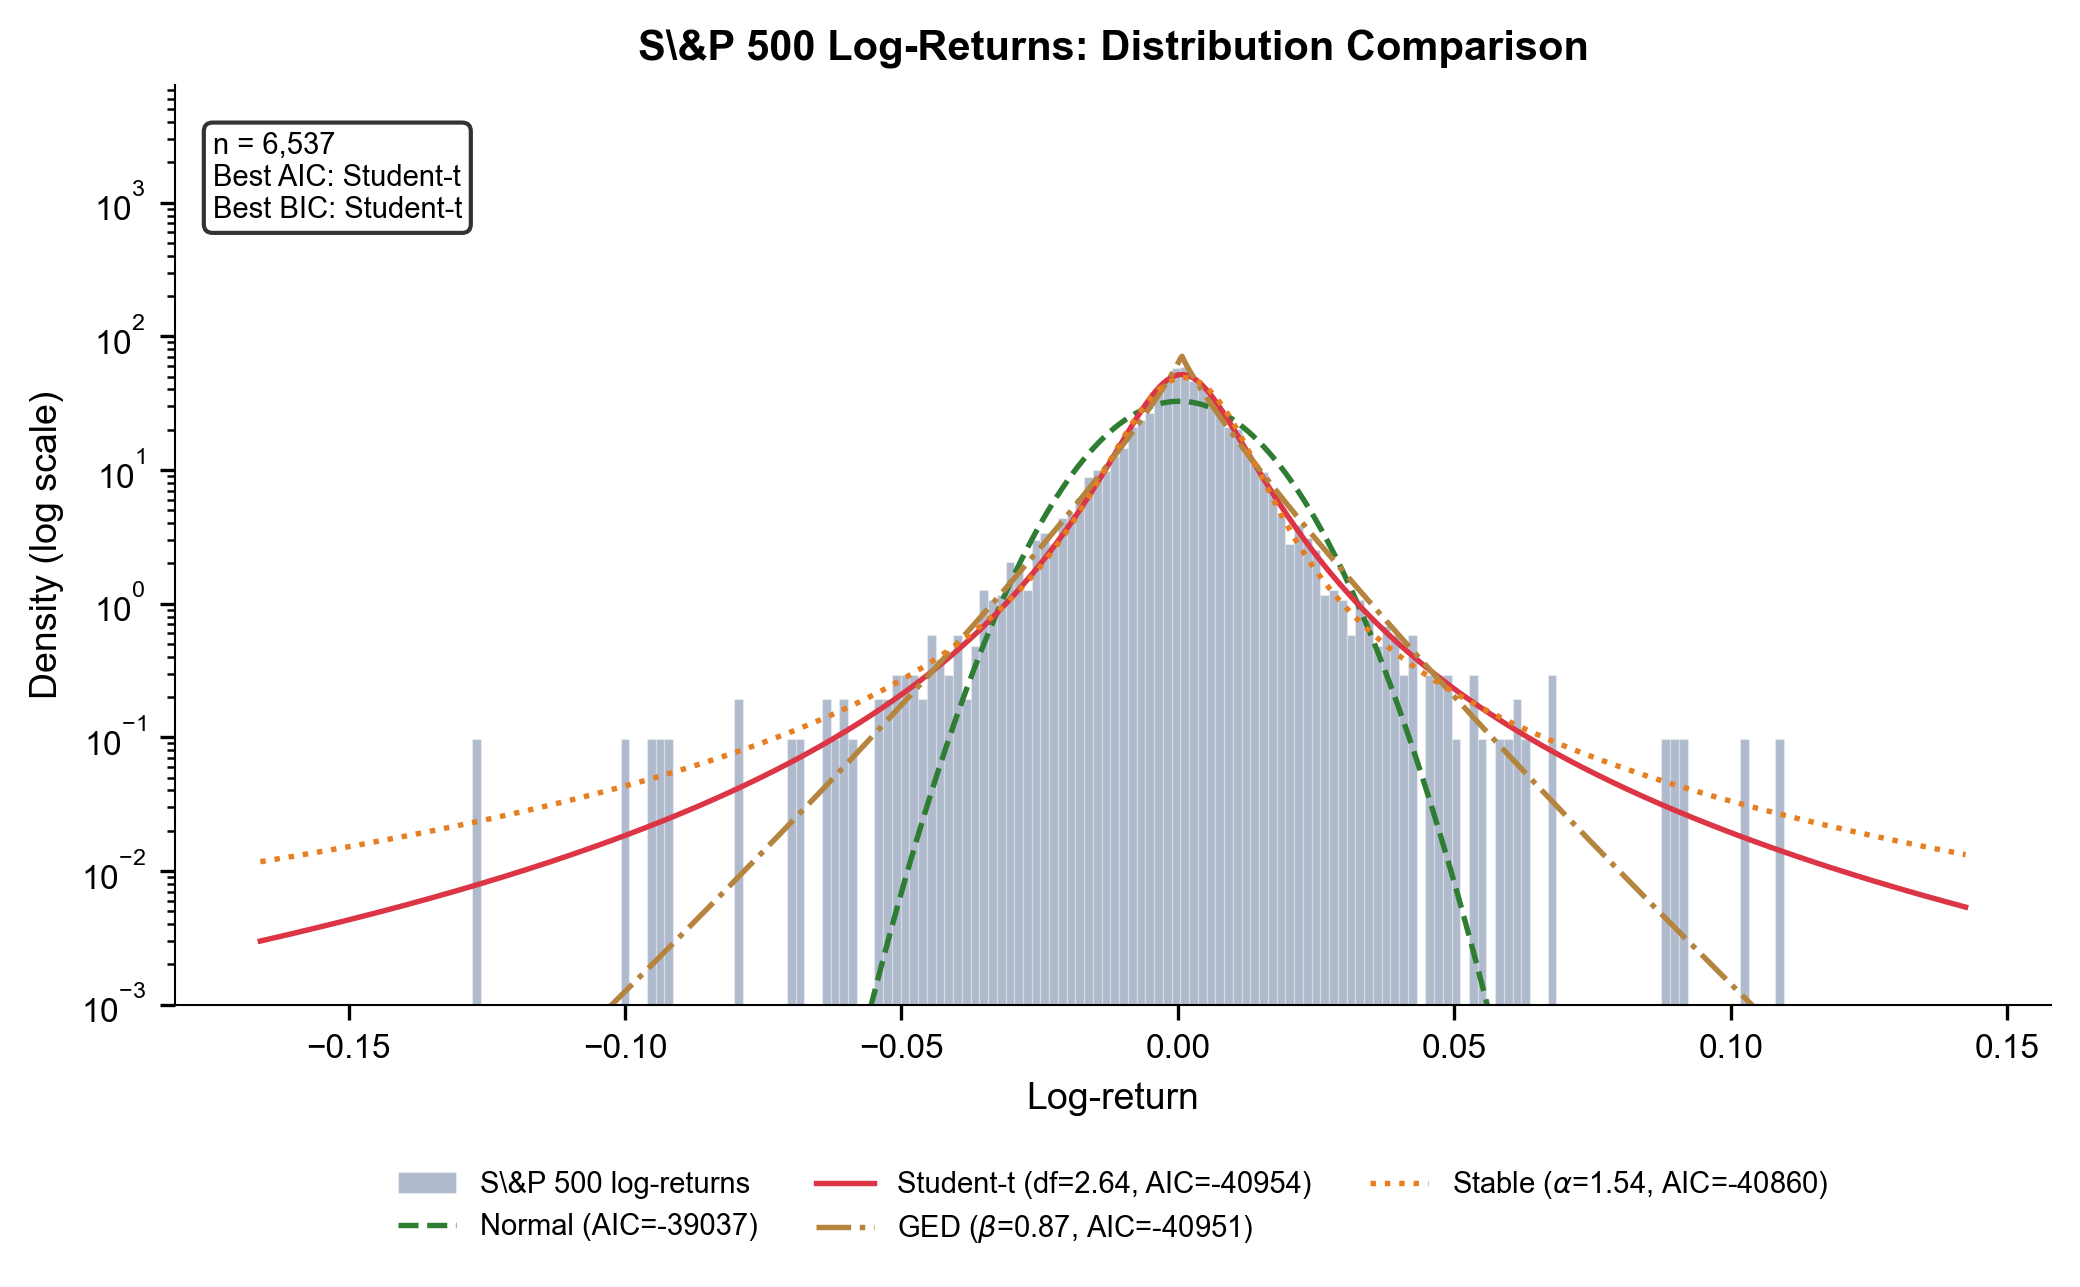
\includegraphics[width=0.40\textwidth]{ch2_dist_comparison_overlay.png}
\end{center}
\vspace{-0.3cm}
\begin{center}
\renewcommand{\arraystretch}{1.0}
\scriptsize
\begin{tabular}{lccc}
\toprule
\textbf{Model} & \textbf{Log-lik} & \textbf{AIC} & \textbf{BIC} \\
\midrule
Normal $(\mu, \sigma)$ & $\ell_1$ & $-2\ell_1 + 4$ & $-2\ell_1 + 2\ln n$ \\
Student-$t$ $(\mu, \sigma, \nu)$ & $\ell_2 > \ell_1$ & $-2\ell_2 + 6$ & $-2\ell_2 + 3\ln n$ \\
\bottomrule
\end{tabular}
\end{center}
\begin{itemize}
\item Student-$t$ achieves substantially better AIC/BIC despite one extra parameter
\end{itemize}
\end{frame}

%--- PhD Slide 7 ---
\begin{frame}{Mixture Representation and Bayesian Interpretation}
\begin{itemize}
\item \textbf{Mixture representation}: $X \mid V \sim N(0, V)$, \quad $V \sim \text{Inv-Gamma}(\nu/2, \nu/2)$
\begin{itemize}
\item Student-$t$ = Normal with random variance (scale mixture of normals)
\item Interpretation: $V$ captures time-varying volatility
\end{itemize}
\item \textbf{Bayesian interpretation}: Student-$t$ as marginal posterior under conjugate normal--inverse-gamma prior
\item \textbf{Multivariate Student-$t$}: $f(\bm{x}) \propto \left(1 + \frac{(\bm{x}-\bm{\mu})'\bm{\Sigma}^{-1}(\bm{x}-\bm{\mu})}{\nu}\right)^{-(\nu+p)/2}$
\item \textbf{Tail comparison}: $t_\nu$ tail index $= \nu$ vs.\ stable tail index $= \alpha$
\item Student-$t$ is \textbf{not} closed under convolution; stable distributions \textbf{are}
\end{itemize}
\end{frame}

%#############################################################################
\section{The Pareto Distribution}
%#############################################################################

%--- Y3 Slide P0: Pareto story ---
\begin{frame}{The 80/20 Rule --- The Man Behind the Law}
\vspace{-0.2cm}
\begin{columns}[T]
\begin{column}{0.28\textwidth}
\begin{center}
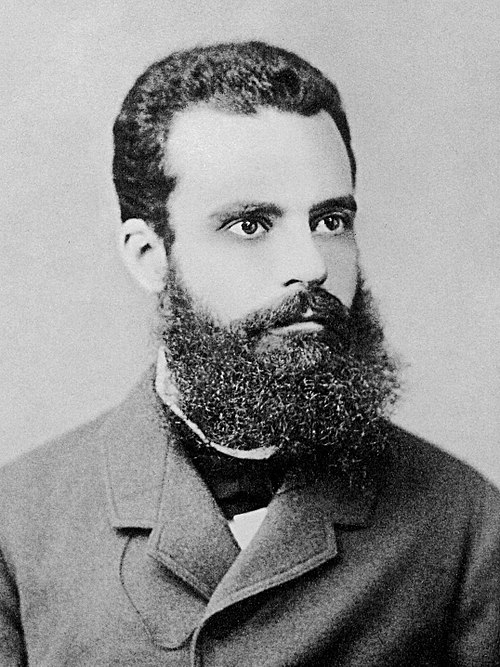
\includegraphics[width=0.78\textwidth]{pareto.jpg}\\[2pt]
{\scriptsize Vilfredo Pareto\\(1848--1923)}
\end{center}
\end{column}
\begin{column}{0.69\textwidth}
\begin{block}{From gardening to inequality}
\begin{itemize}\setlength\itemsep{0pt}
\item Italian-Swiss engineer: \textbf{80\% of Italy's land} was owned by \textbf{20\% of the population} (1896)
\item Legend: 20\% of plants produced 80\% of peas
\item The same law appears \textbf{everywhere}: wealth, cities, earthquakes, sales, web traffic
\end{itemize}
\end{block}
\begin{alertblock}{Why does it matter for finance?}
\begin{itemize}\setlength\itemsep{0pt}
\item A few catastrophic days generate most of the risk
\item Mandelbrot (1963): return tails are Pareto --- $P(X > x) \propto x^{-\alpha}$
\end{itemize}
\end{alertblock}
\end{column}
\end{columns}
\end{frame}

%--- Y3 Slide P1 ---
\begin{frame}{The Pareto Distribution --- Power Law}
\begin{block}{Definition (Pareto, 1896)}
A random variable $X$ follows a \textbf{Pareto distribution} with parameters $x_m > 0$ (scale) and $\alpha > 0$ (shape / tail index) if:
\[
\boxed{\;f(x) = \frac{\alpha\, x_m^\alpha}{x^{\alpha+1}}, \quad x \geq x_m\;}
\]
\end{block}

\begin{columns}[T]
\begin{column}{0.48\textwidth}
\begin{itemize}\setlength\itemsep{2pt}
\item \textbf{CDF}: $F(x) = 1 - \left(\frac{x_m}{x}\right)^\alpha$
\item \textbf{Survival function}:
\[
\bar{F}(x) = P(X > x) = \left(\frac{x_m}{x}\right)^\alpha
\]
\item \textbf{Power-law} behavior: $P(X > x) \propto x^{-\alpha}$
\end{itemize}
\end{column}
\begin{column}{0.48\textwidth}
\begin{itemize}\setlength\itemsep{2pt}
\item \textbf{Mean}: $\E[X] = \frac{\alpha\, x_m}{\alpha - 1}$ \quad (exists only if $\alpha > 1$)
\item \textbf{Variance}: $\Var(X) = \frac{\alpha\, x_m^2}{(\alpha-1)^2(\alpha-2)}$ \quad (exists only if $\alpha > 2$)
\item $\alpha \leq 2$: \textbf{infinite variance}
\item $\alpha \leq 1$: \textbf{infinite mean}
\end{itemize}
\end{column}
\end{columns}
\end{frame}

%--- Y3 Slide P1b: Pareto PDF and CDF chart ---
\begin{frame}{The Pareto Distribution --- PDF and CDF}
\vspace{-0.2cm}
\begin{center}
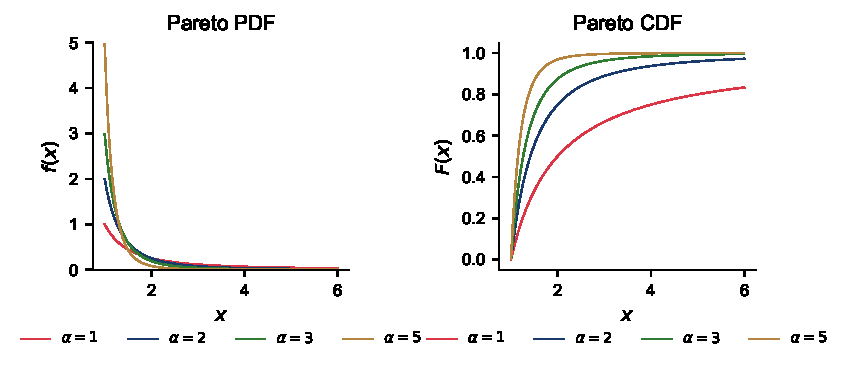
\includegraphics[width=0.78\textwidth]{ch2_pareto_pdf_cdf.pdf}
\end{center}
\vspace{-0.4cm}
\quantlet{SFM\_ch2\_pareto\_analysis}{https://github.com/QuantLet/Stat_fin_markets/tree/master/Ch_02/SFM_ch2_pareto_analysis}
\vspace{-0.1cm}
\begin{itemize}\setlength\itemsep{1pt}
\item Small $\alpha$ $\Rightarrow$ heavy tail, density decays slowly
\item Large $\alpha$ $\Rightarrow$ mass concentrates near $x_m$, tail decays rapidly
\end{itemize}
\end{frame}

%--- Y3 Slide P1c: Log-log survival ---
\begin{frame}{The Pareto Distribution --- Power-Law Signature}
\quantlet{SFM\_ch2\_pareto\_analysis}{https://github.com/QuantLet/Stat_fin_markets/tree/master/Ch_02/SFM_ch2_pareto_analysis}
\begin{block}{Log-log graphical test}
\begin{itemize}\setlength\itemsep{2pt}
\item On a log-log plot, the Pareto survival function is a \textbf{straight line}:
\[
\log P(X > x) = -\alpha \log x + \alpha \log x_m
\]
\vspace{-0.4cm}
\item \textbf{Slope} = $-\alpha$ (tail index)
\item Alignment on a line $\Rightarrow$ Pareto behavior; deviation for small $x$: \textit{truncation}
\item Practical check: plot $\log \hat{S}(x)$ vs.\ $\log x$ on empirical data --- linearity confirms a Pareto tail
\end{itemize}
\end{block}
\end{frame}

%--- Y3 Slide P1c2: Chart full ---
\begin{frame}{The Pareto Distribution --- Log-log Survival}
\begin{center}
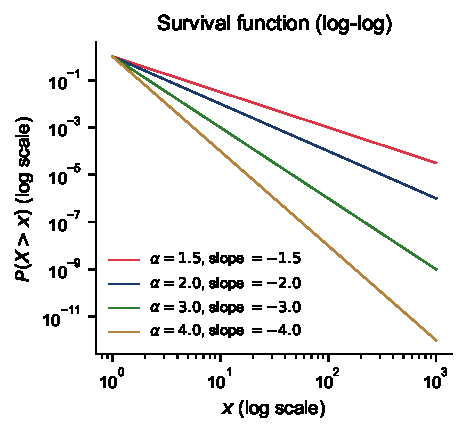
\includegraphics[width=0.75\textwidth]{ch2_pareto_loglog_survival.pdf}
\end{center}
\vspace{-0.3cm}
\quantlet{SFM\_ch2\_pareto\_analysis}{https://github.com/QuantLet/Stat_fin_markets/tree/master/Ch_02/SFM_ch2_pareto_analysis}
\end{frame}

%--- Y3 Slide P2 ---
\begin{frame}{The Pareto Distribution --- Why It Matters in Finance}
\begin{block}{The Pareto principle (80/20 rule)}
\begin{itemize}\setlength\itemsep{1pt}
\item \textbf{Vilfredo Pareto} (1896): 80\% of Italy's wealth was held by 20\% of the population
\item The same law appears in finance: extreme losses follow a power law
\item \textbf{Mandelbrot} (1963): market returns have Pareto-type tails
\end{itemize}
\end{block}
\begin{block}{Key property: heavy tails}
\begin{itemize}\setlength\itemsep{1pt}
\item Normal: $P(X > x) \sim e^{-x^2/2}$ (\textbf{exponential}); Pareto: $P(X > x) \sim x^{-\alpha}$ (\textbf{polynomial})
\item \textit{Black Swan} events are \textbf{much more probable} under Pareto
\item \textbf{Example}: $\alpha = 3$, $P(X > 10 x_m) = 10^{-3}$; under Normal: $\approx 10^{-23}$
\end{itemize}
\end{block}
\end{frame}

%--- Y3 Slide P2b: MLE ---
\begin{frame}{The Pareto Distribution --- Parameter Estimation (MLE)}
\begin{block}{Maximum Likelihood Estimator (MLE)}
\begin{itemize}\setlength\itemsep{2pt}
\item Let $x_1, \ldots, x_n$ be an i.i.d.\ sample from $\text{Pareto}(\alpha, x_m)$
\item \textbf{Step 1}: $\hat{x}_m = \min(x_1, \ldots, x_n)$ \quad (scale = minimum value)
\item \textbf{Step 2}: $\displaystyle\hat{\alpha}_{\text{MLE}} = \frac{n}{\sum_{i=1}^{n} \ln(x_i / \hat{x}_m)}$
\item \textbf{Properties}: consistent, asymptotically efficient, $\sqrt{n}$-convergent
\end{itemize}
\end{block}
\end{frame}

%--- Y3 Slide P2b2: MLE demo chart ---
\begin{frame}{The Pareto Distribution --- MLE: Demonstration}
\vspace{-0.2cm}
\begin{center}
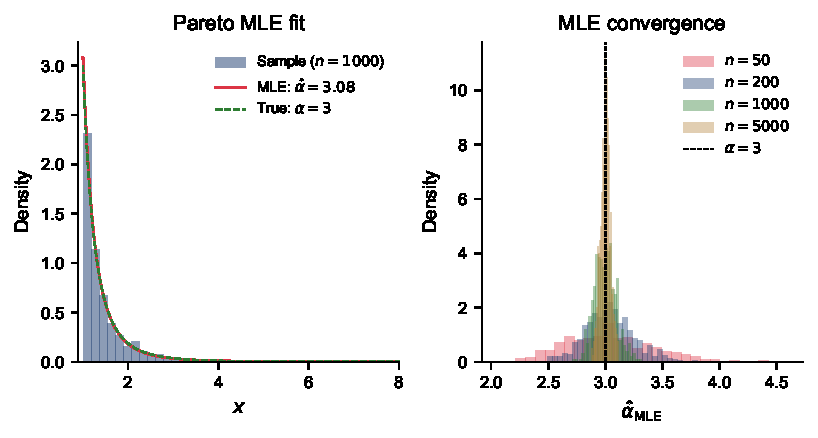
\includegraphics[width=0.78\textwidth]{ch2_pareto_mle_demo.pdf}
\end{center}
\vspace{-0.3cm}
\quantlet{SFM\_ch2\_pareto\_analysis}{https://github.com/QuantLet/Stat_fin_markets/tree/master/Ch_02/SFM_ch2_pareto_analysis}
\vspace{-0.1cm}
\begin{itemize}\setlength\itemsep{1pt}
\item \textbf{Left}: histogram + MLE fit vs.\ true value ($\alpha = 3$, $n = 1000$)
\item \textbf{Right}: MLE convergence as $n$ increases ($n = 50 \to 5000$)
\end{itemize}
\end{frame}

%--- MSc Slide P2c: Hill estimator on S&P 500 ---
\begin{frame}{The Pareto Distribution --- Hill Estimator on S\&P~500}
\vspace{-0.2cm}
\begin{center}
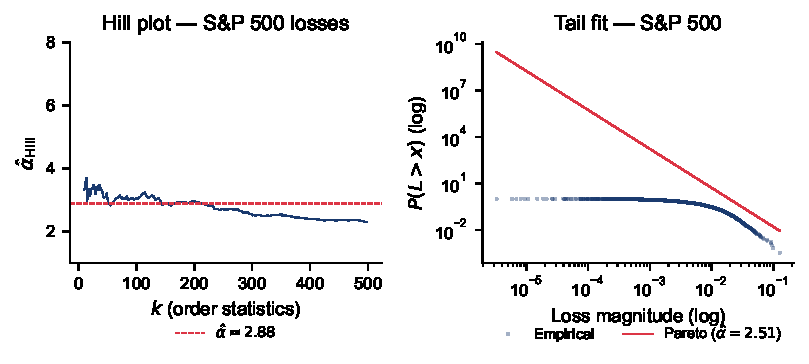
\includegraphics[width=0.80\textwidth]{ch2_pareto_hill_sp500.pdf}
\end{center}
\vspace{-0.3cm}
\quantlet{SFM\_ch2\_pareto\_analysis}{https://github.com/QuantLet/Stat_fin_markets/tree/master/Ch_02/SFM_ch2_pareto_analysis}
\vspace{-0.1cm}
\begin{itemize}\setlength\itemsep{1pt}
\item \textbf{Hill plot}: stable region $\hat{\alpha} \approx 2.9$; \textbf{Tail fit}: Pareto $\hat{\alpha} \approx 2.5$
\item $\alpha < 3$ $\Rightarrow$ moments of order $\geq 3$ do not exist; confirmation: \textbf{heavy tails}
\end{itemize}
\end{frame}

%--- MSc Slide P2c2: Tail fitting chart ---
\begin{frame}{The Pareto Distribution --- Tail Fitting (S\&P~500)}
\begin{center}
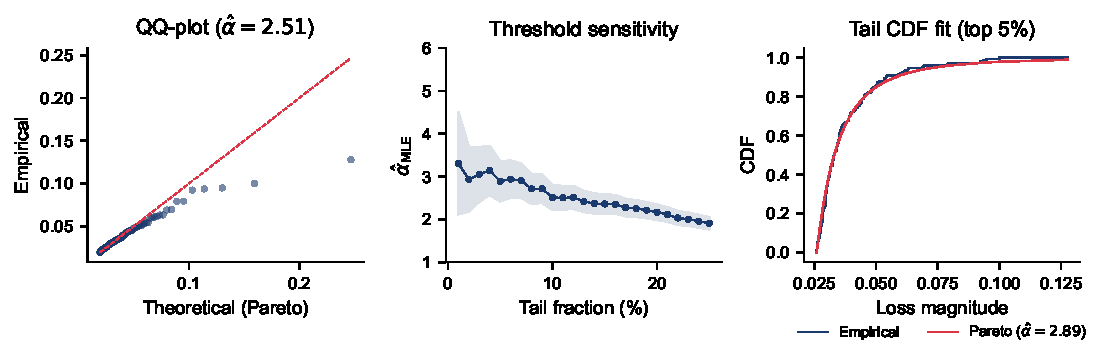
\includegraphics[width=0.85\textwidth]{ch2_pareto_tail_fitting.pdf}
\end{center}
\vspace{-0.3cm}
\quantlet{SFM\_ch2\_pareto\_analysis}{https://github.com/QuantLet/Stat_fin_markets/tree/master/Ch_02/SFM_ch2_pareto_analysis}
\begin{itemize}\setlength\itemsep{2pt}
\item \textbf{QQ-plot}: alignment on diagonal $\Rightarrow$ tail is Pareto
\item \textbf{Threshold sensitivity}: stable region $\approx$ 3--8\%; $\hat{\alpha} \approx 2.5$--$3.0$
\end{itemize}
\end{frame}

%--- MSc Slide P2c3: Tail fitting interpretation ---
\begin{frame}{The Pareto Distribution --- Tail Fitting Interpretation}
\begin{block}{Tail fitting procedure}
\begin{itemize}\setlength\itemsep{2pt}
\item \textbf{Step 1}: Select threshold $u$ (or tail fraction, e.g.\ top 5\%)
\item \textbf{Step 2}: Estimate $\hat{\alpha}$ on data $\{x_i : x_i > u\}$ via MLE or Hill
\item \textbf{Step 3}: Check sensitivity: vary $u$ and observe $\hat{\alpha}$ stability
\item \textbf{Step 4}: Validate with QQ-plot and CDF fit
\end{itemize}
\end{block}
\begin{alertblock}{Empirical results (S\&P~500, 2000--2025)}
\begin{itemize}\setlength\itemsep{2pt}
\item $\hat{\alpha} \approx 2.5$--$3.0$ $\Rightarrow$ finite moments only up to order 2
\item Variance exists, but kurtosis \textbf{does not} --- the Normal distribution is inadequate
\item The Pareto CDF fits well on the right tail of losses
\end{itemize}
\end{alertblock}
\end{frame}

%--- Y3 Slide P2d: Applications ---
\begin{frame}{The Pareto Distribution --- Applications}
\quantlet{SFM\_ch2\_pareto\_analysis}{https://github.com/QuantLet/Stat_fin_markets/tree/master/Ch_02/SFM_ch2_pareto_analysis}
\begin{block}{Zipf's law (market capitalization)}
\begin{itemize}\setlength\itemsep{2pt}
\item Firm capitalization follows a \textbf{power law}: $P(\text{cap} > x) \propto x^{-\alpha}$
\item Top 10 firms $\approx$ 30\% of the market; Zipf slope $\approx -1$ (universal empirical law)
\end{itemize}
\end{block}
\begin{block}{Other applications of the Pareto distribution}
\begin{itemize}\setlength\itemsep{2pt}
\item \textbf{Insurance losses}: extreme insured amounts $\Rightarrow$ Pareto
\item \textbf{Operational risk} (Basel~II): operational losses have Pareto tails
\item \textbf{Wealth distribution}: Top 1\% holds 40--50\% of wealth (Piketty, 2014)
\item \textbf{Trading volume}: a few large trades dominate total volume
\item \textbf{Cyber risk}: severity of cyber attacks is Pareto-distributed
\end{itemize}
\end{block}
\end{frame}

%--- Y3 Slide P2d2: Zipf chart ---
\begin{frame}{Zipf's Law --- Market Capitalization}
\begin{center}
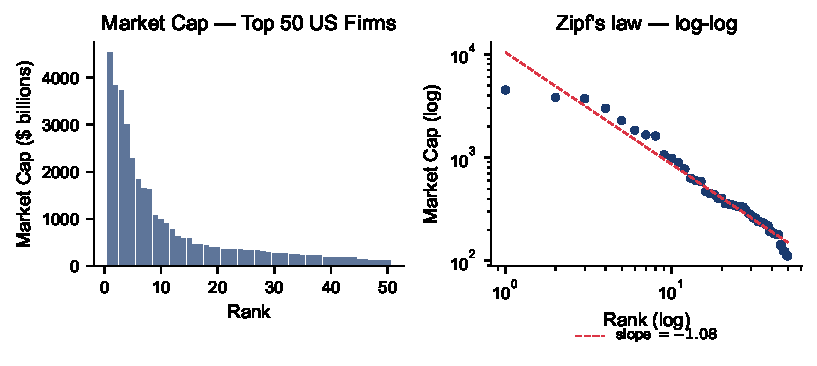
\includegraphics[width=0.82\textwidth]{ch2_pareto_market_cap.pdf}
\end{center}
\vspace{-0.3cm}
\quantlet{SFM\_ch2\_pareto\_analysis}{https://github.com/QuantLet/Stat_fin_markets/tree/master/Ch_02/SFM_ch2_pareto_analysis}
\end{frame}

%--- MSc Slide P3: Theoretical connections ---
\begin{frame}{The Pareto Distribution --- Theoretical Connections}
\small
\vspace{-0.3cm}
\begin{block}{Connection with EVT and the Hill estimator}
\begin{itemize}\setlength\itemsep{1pt}
\item \textbf{Pickands--Balkema--de Haan theorem}: exceedances above a sufficiently high threshold approximately follow a \textbf{Generalized Pareto Distribution} (GPD)
\item The classical Pareto distribution = special case of GPD with $\xi > 0$
\item \textbf{Hill estimator}: estimates $\alpha$ from order statistics $X_{(1)} \leq \cdots \leq X_{(n)}$:
\[
\hat{\alpha}_{\text{Hill}} = \left(\frac{1}{k}\sum_{i=1}^{k} \ln \frac{X_{(n-i+1)}}{X_{(n-k)}}\right)^{-1}
\]
\end{itemize}
\end{block}

\begin{block}{Connection with stable distributions and Student-$t$}
\begin{itemize}\setlength\itemsep{1pt}
\item $\alpha$-stable distributions with $\alpha < 2$ have Pareto tails: $P(X > x) \sim C_\alpha\, x^{-\alpha}$
\item Student-$t$ with $\nu$ degrees of freedom: Pareto tails with index $\alpha = \nu$
\item The Pareto tail index unifies the theory: smaller $\alpha$ $\Rightarrow$ heavier tails
\end{itemize}
\end{block}
\end{frame}

%#############################################################################
% Sections removed: Asymmetric Distributions, Stable Distributions, EVT,
% Distribution Comparison, Risk Management, Modern Extensions
% (covered in separate chapters: Ch.3 Stable, Ch.5 Heavy Tails, etc.)
%#############################################################################

% BULK_REMOVE_START
\begin{itemize}
\item Negative skewness in equity returns: downside risk is larger than upside potential
\item \textbf{Skewness} measures asymmetry: $S = \E[(X-\mu)^3]/\sigma^3$
\item Symmetric distributions (Normal, Student-$t$) assign equal probability to left and right tails
\item But empirically: the left tail of equity returns is \textbf{heavier} than the right tail
\item We need distributions that can distinguish left from right tail behavior
\end{itemize}

\vspace{0.3cm}
\begin{alertblock}{Risk Implication}
\begin{itemize}
\item Ignoring skewness leads to underestimating \textbf{downside risk}
\item A symmetric model with the correct kurtosis still misallocates probability between the two tails
\end{itemize}
\end{alertblock}
\end{frame}

%--- Y3 Slide 2 ---
\begin{frame}{Skewness in Financial Returns}
\begin{center}
\renewcommand{\arraystretch}{1.1}
\begin{tabular}{lcc}
\toprule
\textbf{Asset Class} & \textbf{Typical Skewness} & \textbf{Implication} \\
\midrule
Equity indices & $-0.1$ to $-0.5$ & Heavier left tail \\
Individual stocks & $-0.3$ to $-1.0$ & Strong crash risk \\
FX majors & $\approx 0$ & Approximately symmetric \\
Commodities & Mixed & Depends on supply shocks \\
Bonds & Slightly positive & Right tail (yield spikes) \\
\bottomrule
\end{tabular}
\end{center}

\vspace{0.2cm}
\begin{itemize}
\item Skewness affects 1\% VaR: a left-skewed distribution has a more extreme left quantile than a symmetric distribution with the same variance
\end{itemize}
\end{frame}

%--- MSc Slide 3 ---
\begin{frame}{Hansen's Skewed-$t$ Distribution}
\begin{defn}[Hansen's Skewed-$t$ (Hansen, 1994)]
\[
f(x;\nu,\lambda) = \begin{cases}
bc\!\left(1 + \frac{1}{\nu-2}\left(\frac{bx+a}{1-\lambda}\right)^{\!2}\right)^{-(\nu+1)/2} & x < -a/b \\[6pt]
bc\!\left(1 + \frac{1}{\nu-2}\left(\frac{bx+a}{1+\lambda}\right)^{\!2}\right)^{-(\nu+1)/2} & x \geq -a/b
\end{cases}
\]
where $\lambda \in (-1,1)$ is the skewness parameter, $a = 4\lambda c\frac{\nu-2}{\nu-1}$, $b^2 = 1 + 3\lambda^2 - a^2$, $c = \frac{\Gamma((\nu+1)/2)}{\sqrt{\pi(\nu-2)}\,\Gamma(\nu/2)}$.
\end{defn}

\begin{itemize}
\item $\lambda = 0$: symmetric Student-$t$; \quad $\lambda < 0$: heavier left tail
\item Widely used as GARCH innovation distribution
\end{itemize}
\end{frame}

%--- MSc Slide 4 ---
\begin{frame}{Generalized Error Distribution (GED)}
\begin{defn}[GED]
\[
f(x;\nu) = \frac{\nu}{2\,\Gamma(1/\nu)}\exp\!\left(-|x|^\nu\right), \quad \nu > 0.
\]
\end{defn}

\begin{itemize}
\item $\nu = 2$: Normal distribution; \quad $\nu = 1$: Laplace (double exponential)
\item $\nu < 2$: heavier tails than Normal; \quad $\nu > 2$: lighter tails
\item Controls tail heaviness through a single parameter
\item Popular in GARCH models: GARCH-GED
\end{itemize}

\vspace{0.2cm}
\begin{block}{MLE Estimation}
\begin{itemize}
\item For both skewed-$t$ and GED, estimate parameters via maximum likelihood
\item Compare using AIC/BIC
\end{itemize}
\end{block}
\end{frame}

%--- MSc Slide 5 ---
\begin{frame}{Asymmetric Distribution Comparison}
\begin{center}
\renewcommand{\arraystretch}{1.1}
\begin{tabular}{lccc}
\toprule
\textbf{Distribution} & \textbf{Parameters} & \textbf{Skewness} & \textbf{Tail type} \\
\midrule
Normal & $\mu, \sigma$ & 0 & Exponential \\
Student-$t$ & $\mu, \sigma, \nu$ & 0 & Power law \\
Skewed-$t$ & $\mu, \sigma, \nu, \lambda$ & $\neq 0$ & Power law (asymmetric) \\
GED & $\mu, \sigma, \nu$ & 0 & Stretched exponential \\
NIG & $\alpha, \beta, \delta, \mu$ & $\neq 0$ & Semi-heavy \\
\bottomrule
\end{tabular}
\end{center}

\begin{itemize}
\item More parameters $\Rightarrow$ better fit but risk of overfitting
\item AIC/BIC balance goodness-of-fit against complexity
\item For daily equity returns: skewed-$t$ often dominates
\end{itemize}
\end{frame}

%--- PhD Slide 6 ---
\begin{frame}{The Generalized Hyperbolic Family}
\begin{itemize}
\item \textbf{Generalized Hyperbolic (GH)} distribution: five parameters $(\lambda, \alpha, \beta, \delta, \mu)$
\item PDF:
\[
f(x) \propto \left(\delta^2 + (x-\mu)^2\right)^{(\lambda - 1/2)/2} K_{\lambda-1/2}\!\left(\alpha\sqrt{\delta^2 + (x-\mu)^2}\right) e^{\beta(x-\mu)}
\]
where $K_\nu$ is the modified Bessel function of the second kind
\item Special cases:
\begin{itemize}
\item \textbf{Hyperbolic}: $\lambda = 1$
\item \textbf{NIG} (Normal Inverse Gaussian): $\lambda = -1/2$
\item \textbf{VG} (Variance Gamma): $\delta \to 0$
\end{itemize}
\end{itemize}
\end{frame}

%--- PhD Slide 7 ---
\begin{frame}{Normal Mean-Variance Mixtures}
\begin{itemize}
\item \textbf{GH as normal mean-variance mixture}:
\[
X \mid W \sim N(\mu + \beta W, W), \quad W \sim \text{GIG}(\lambda, \delta, \gamma)
\]
where GIG is the Generalized Inverse Gaussian distribution
\item Barndorff-Nielsen (1977): excellent empirical fit to financial data
\item \textbf{Affine closure}: GH distributions are closed under affine transformations
\item Multivariate GH: tractable for portfolio problems
\item Connection to L\'{e}vy processes: GH distributions are infinitely divisible $\Rightarrow$ GH L\'{e}vy processes
\end{itemize}
\end{frame}

%#############################################################################
\section{Stable ($\alpha$-Stable) Distributions}
%#############################################################################

%--- Y3 Slide 1 ---
\begin{frame}{What Is a Stable Distribution?}
\begin{defn}[Stable Distribution --- Intuitive]
A distribution is \textbf{stable} if a sum of i.i.d.\ copies has the same shape (up to location and scale). Formally, $X \sim S(\alpha, \beta, \gamma, \delta)$ if for i.i.d.\ copies $X_1, X_2$:
\[
aX_1 + bX_2 \stackrel{d}{=} cX + d, \quad c = (a^\alpha + b^\alpha)^{1/\alpha}.
\]
\end{defn}

\begin{itemize}
\item \textbf{Four parameters}:
\begin{itemize}
\item $\alpha \in (0, 2]$: \textbf{stability index} (tail heaviness) --- smaller $\alpha$ $\Rightarrow$ heavier tails
\item $\beta \in [-1, 1]$: \textbf{skewness}
\item $\gamma > 0$: \textbf{scale}
\item $\delta \in \R$: \textbf{location}
\end{itemize}
\item Special cases: $\alpha = 2$ (Gaussian), $\alpha = 1, \beta = 0$ (Cauchy)
\end{itemize}
\end{frame}

%--- Y3 Slide 2 ---
\begin{frame}{Why Variance May Not Exist}
\begin{itemize}
\item For $\alpha < 2$: $\E[|X|^p] < \infty$ if and only if $p < \alpha$
\item In particular, $\E[X^2] = \infty$ when $\alpha < 2$ --- the \textbf{variance does not exist}
\item The sample variance does not converge to a constant; it grows with $n$
\item \textbf{Mandelbrot (1963)}: cotton price changes follow stable laws with $\alpha \approx 1.7$
\item Typical estimates for financial returns: $\hat{\alpha} \in [1.5, 1.9]$
\end{itemize}

\vspace{0.2cm}
\begin{alertblock}{Paradigm Shift}
\begin{itemize}
\item If returns are truly stable with $\alpha < 2$, then classical portfolio theory (Markowitz mean-variance) breaks down
\item Variance is not a meaningful risk measure when $\alpha < 2$
\end{itemize}
\end{alertblock}
\end{frame}

%--- Y3 Slide 3 ---
\begin{frame}{Stable Fit to S\&P 500}
\quantlet{SFM\_ch2\_stable\_fit}{https://github.com/QuantLet/SFM/tree/master/QID-3447-SFMstable}
\begin{center}
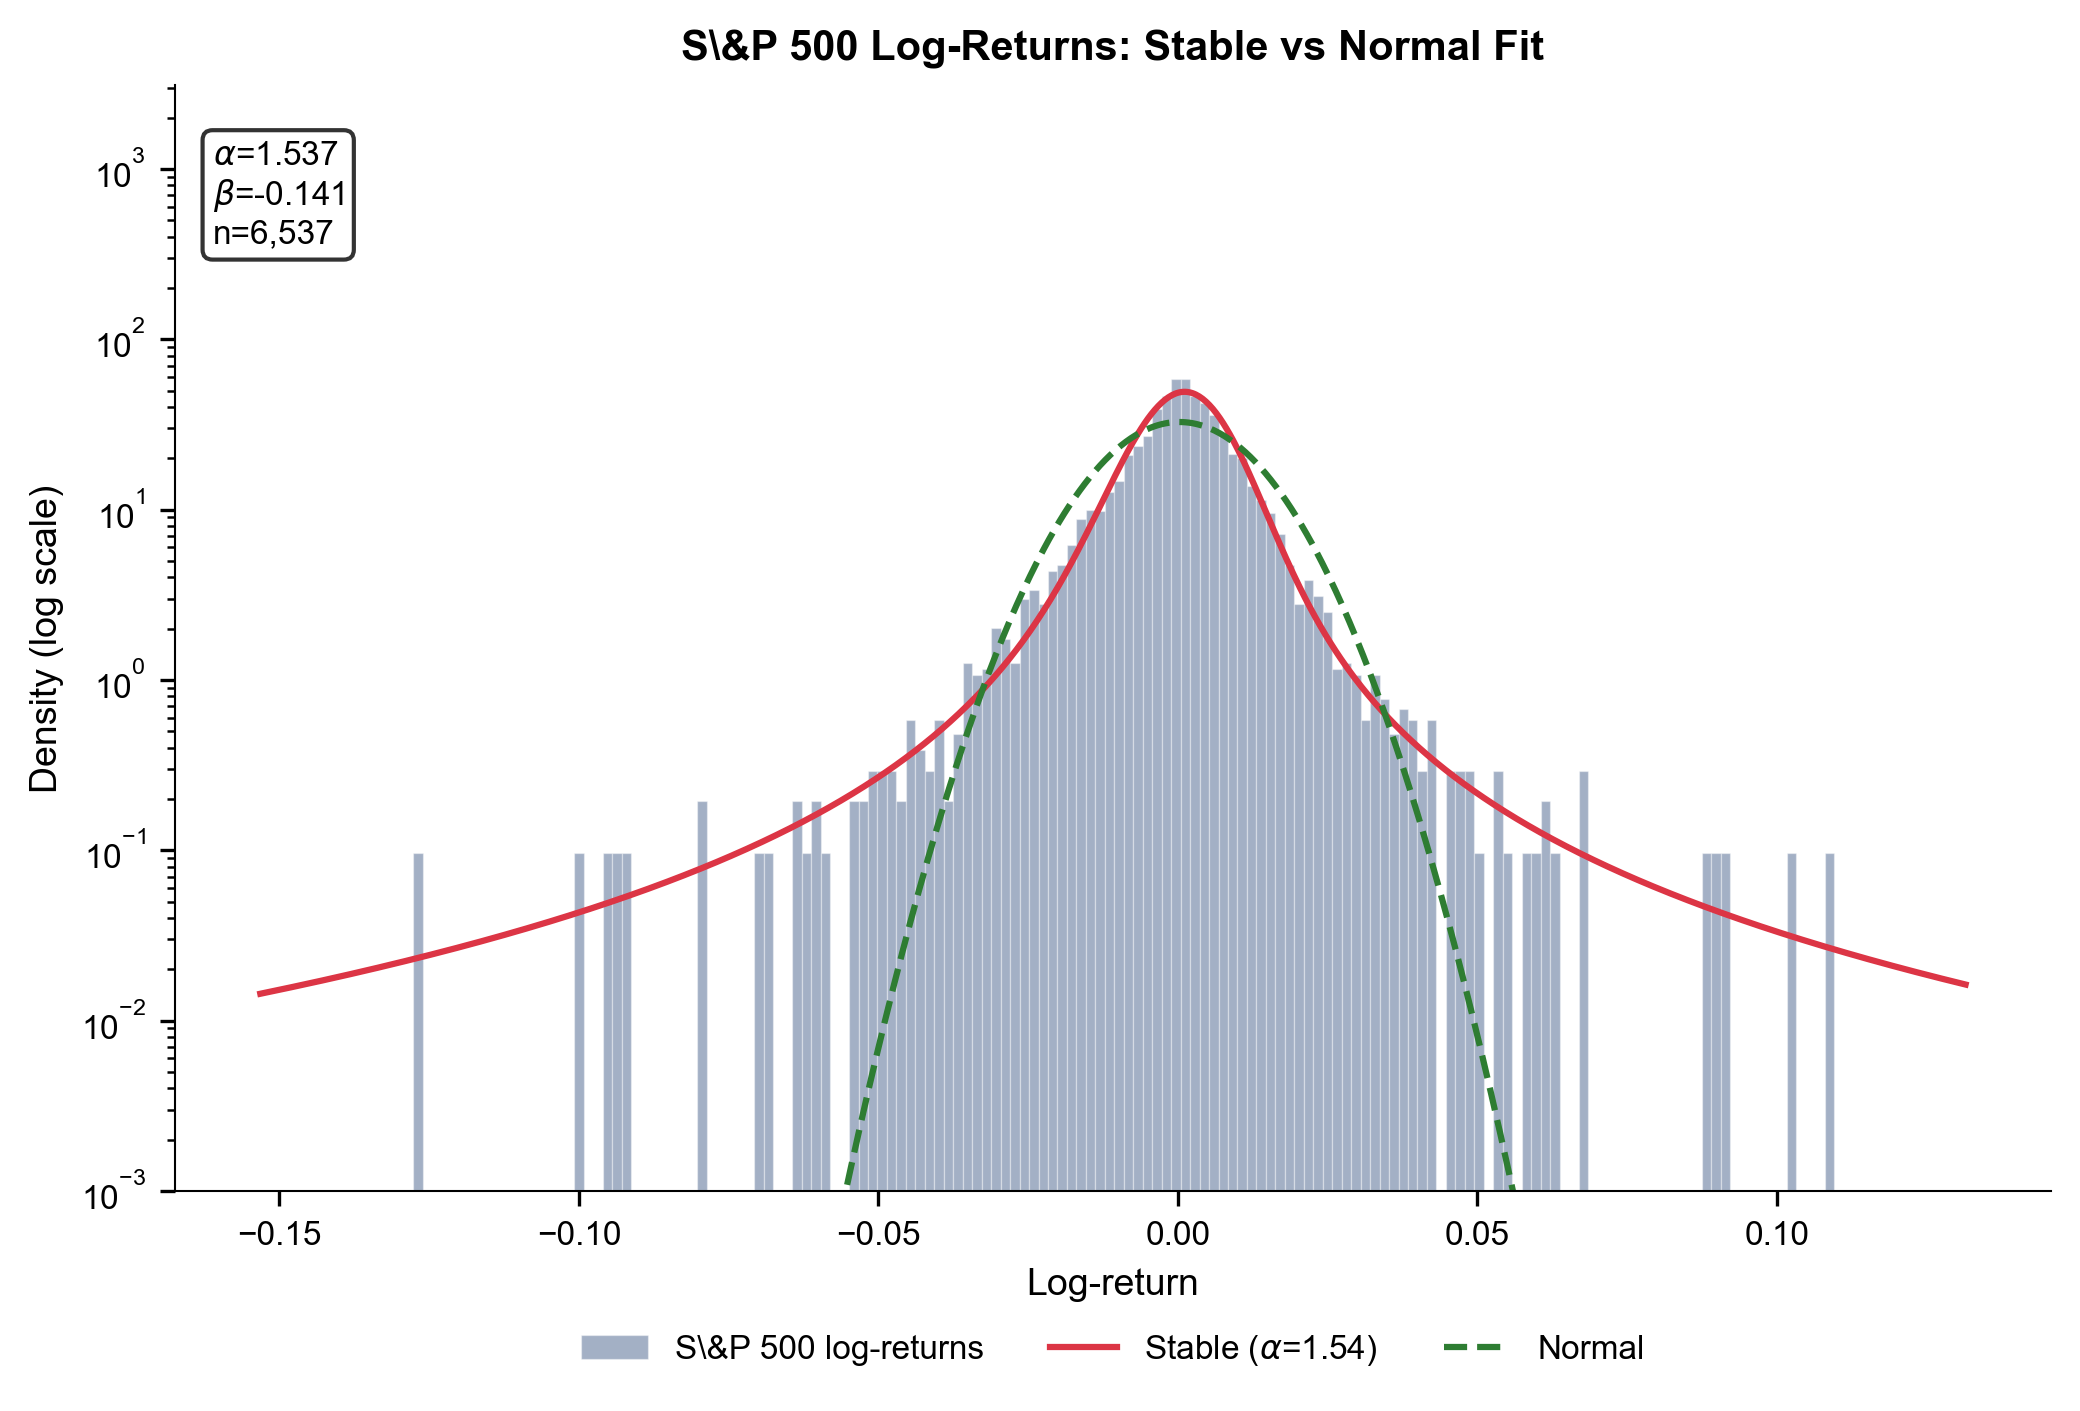
\includegraphics[width=0.5\textwidth]{ch2_sp500_stable_fit.png}
\end{center}
\begin{itemize}
\item Stable distribution captures heavy tails better than Normal
\item Estimated $\hat{\alpha} \approx 1.7$ for S\&P~500 daily returns
\end{itemize}
\end{frame}

%--- Y3 Slide 4 ---
\begin{frame}{Stable vs.\ Normal vs.\ Student-$t$}
\begin{center}
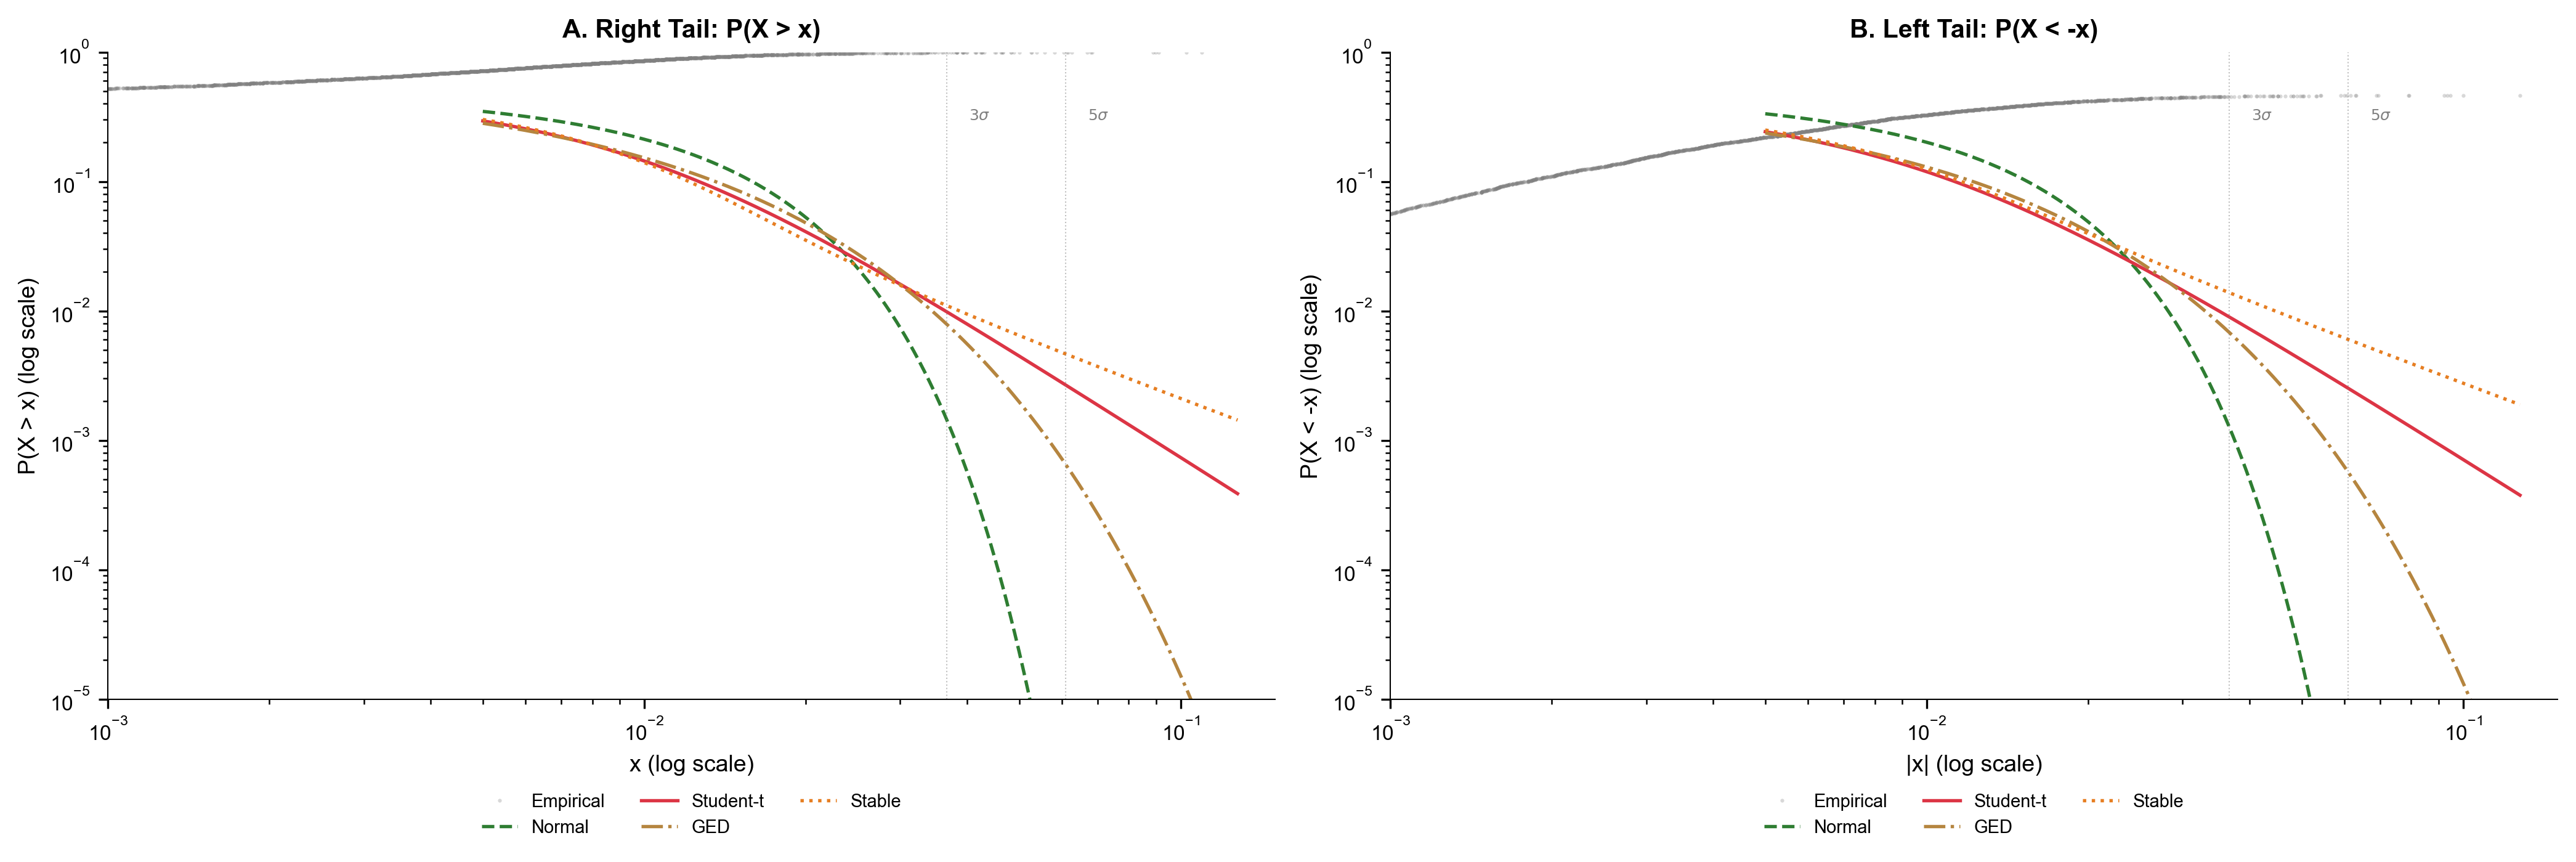
\includegraphics[width=0.65\textwidth]{ch2_dist_comparison_tails.png}
\end{center}

\begin{center}
\renewcommand{\arraystretch}{1.1}
\begin{tabular}{lccc}
\toprule
& \textbf{Normal} & \textbf{Student-$t$} & \textbf{Stable} \\
\midrule
Tail decay & $e^{-x^2/2}$ & $|x|^{-\nu-1}$ & $|x|^{-\alpha}$ \\
Variance & Finite & Finite ($\nu>2$) & Infinite ($\alpha<2$) \\
Closed under sum & Yes & No & Yes \\
CLT limit & CLT & --- & GCLT \\
\bottomrule
\end{tabular}
\end{center}
\end{frame}

%--- MSc Slide 5 ---
\begin{frame}{Characteristic Function}
The stable distribution is defined via its \textbf{characteristic function} ($\alpha \neq 1$):
\[
\phi(t) = \E[e^{itX}] = \exp\!\left\{-\gamma^\alpha |t|^\alpha\!\left(1 - i\beta\,\text{sign}(t)\tan\frac{\pi\alpha}{2}\right) + i\delta t\right\}
\]
Case $\alpha = 1$:
\[
\phi(t) = \exp\!\left\{-\gamma|t|\!\left(1 + i\beta\frac{2}{\pi}\,\text{sign}(t)\ln|t|\right) + i\delta t\right\}
\]

\begin{itemize}
\item \textbf{No closed-form PDF} in general (exceptions: Gaussian, Cauchy, L\'{e}vy)
\item Density via inverse Fourier transform: $f(x) = \frac{1}{2\pi}\int_{-\infty}^{\infty}\phi(t)\,e^{-itx}\,dt$
\item Numerical evaluation: Nolan's algorithm (1997)
\end{itemize}
\end{frame}

%--- MSc Slide 6 ---
\begin{frame}{Generalized Central Limit Theorem}
\begin{thm}[GCLT]
Stable distributions are the \textit{only} possible non-degenerate limits of normalized sums:
\[
\frac{S_n - b_n}{a_n} \xrightarrow{d} S(\alpha, \beta, \gamma, \delta)
\]
where $S_n = X_1 + \cdots + X_n$ for i.i.d.\ $X_i$.
\end{thm}

\begin{itemize}
\item Classical CLT: $\alpha = 2$ (requires finite variance)
\item GCLT: $\alpha < 2$ (allows infinite variance)
\item \textbf{Stability property}: Sums of i.i.d.\ stable r.v.'s remain stable with the same $\alpha$
\item \textbf{Power-law tails}: $P(X > x) \sim C_\alpha(1+\beta)\,x^{-\alpha}$ as $x \to \infty$
\end{itemize}
\end{frame}

%--- MSc Slide 7 ---
\begin{frame}{Stable PDFs --- Varying $\alpha$}
\begin{center}
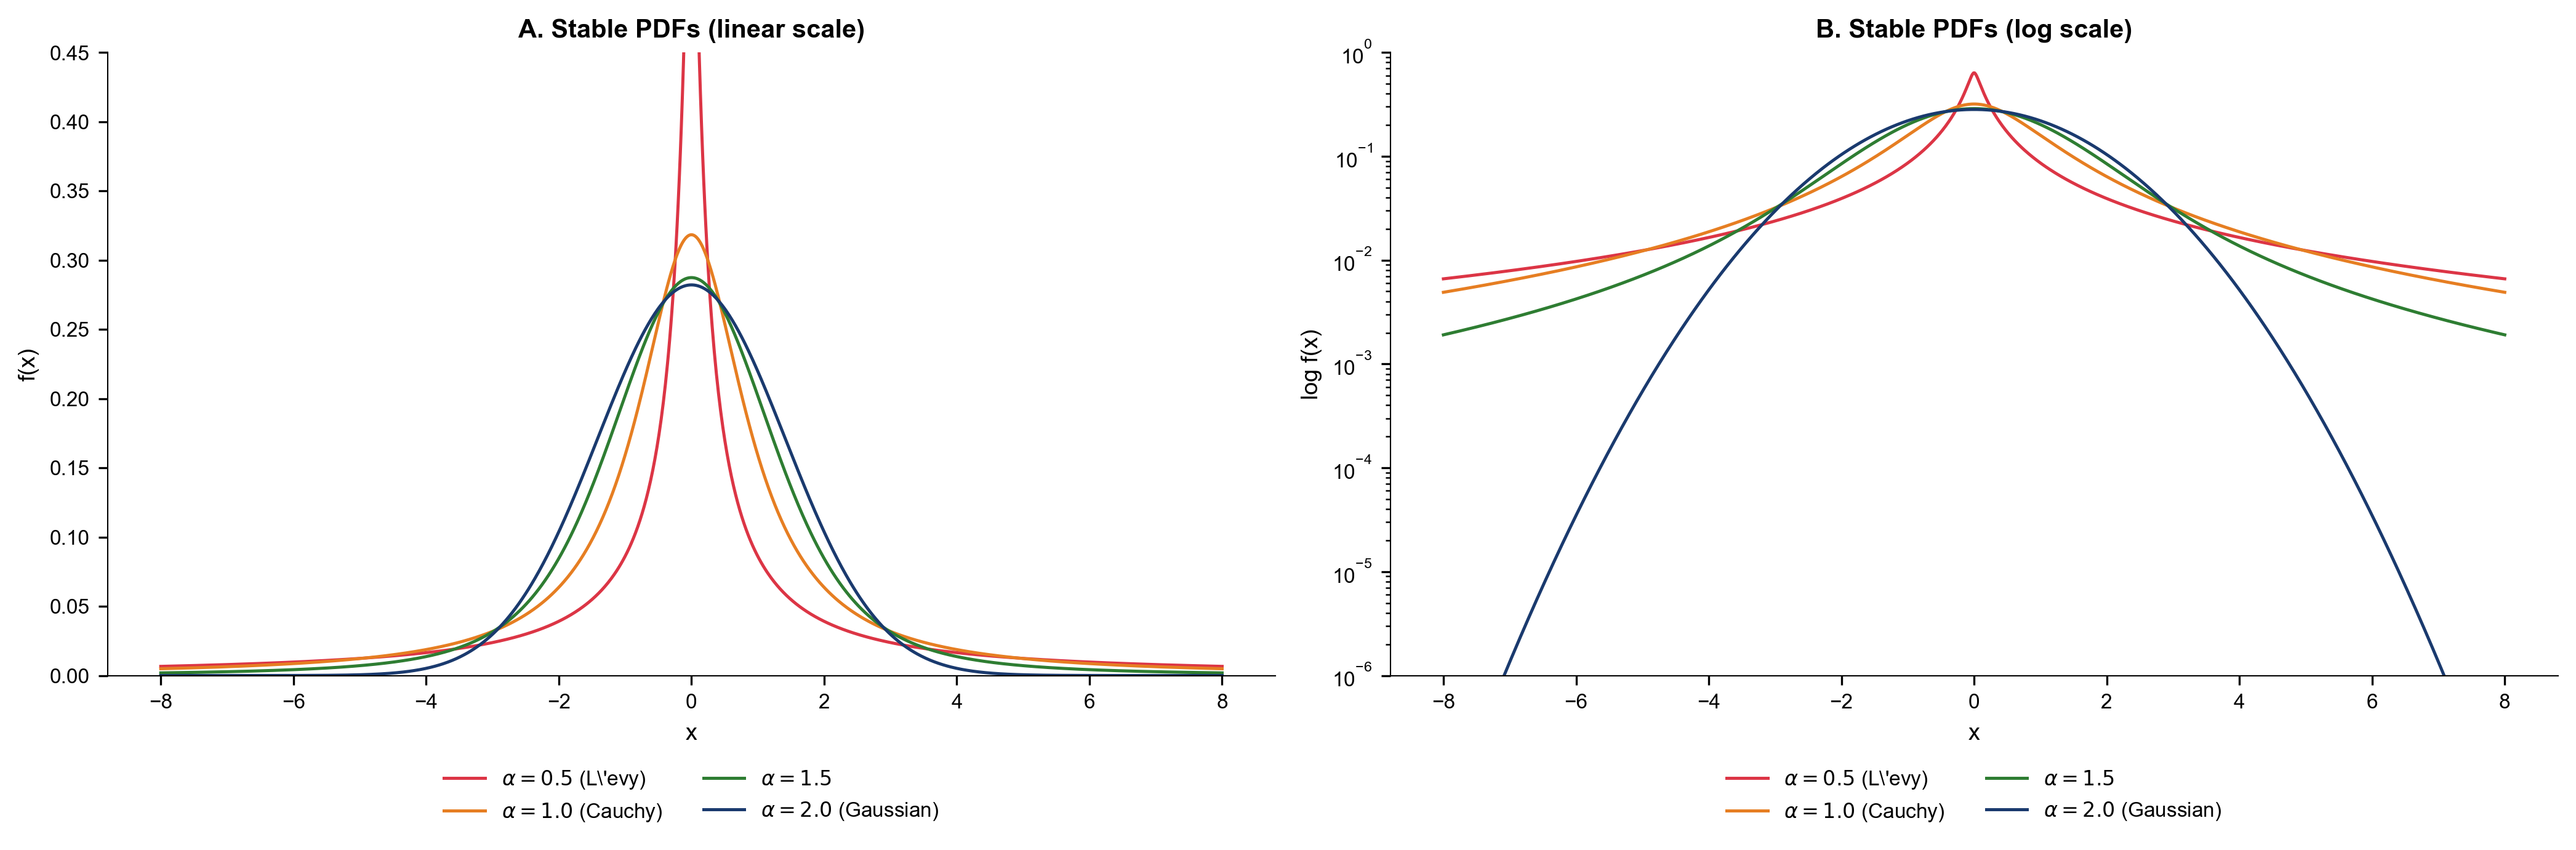
\includegraphics[width=0.72\textwidth]{ch2_stable_pdfs.png}
\end{center}

\begin{itemize}
\item Smaller $\alpha$ $\Rightarrow$ heavier tails, sharper peak
\item $\alpha = 2$: Gaussian; $\alpha = 1$: Cauchy
\item Financial returns: $\hat{\alpha} \in [1.5, 1.9]$
\end{itemize}
\end{frame}

%--- MSc Slide 8 ---
\begin{frame}{Estimation and Cross-Asset Analysis}
\begin{columns}[T]
\begin{column}{0.48\textwidth}
\textbf{Estimation methods}:
\begin{itemize}
\item McCulloch quantile method (quick, consistent)
\item MLE (Nolan, 1997) --- most efficient
\item Characteristic function methods (Kogon \& Williams, 1998)
\end{itemize}
\end{column}
\begin{column}{0.48\textwidth}
\begin{center}
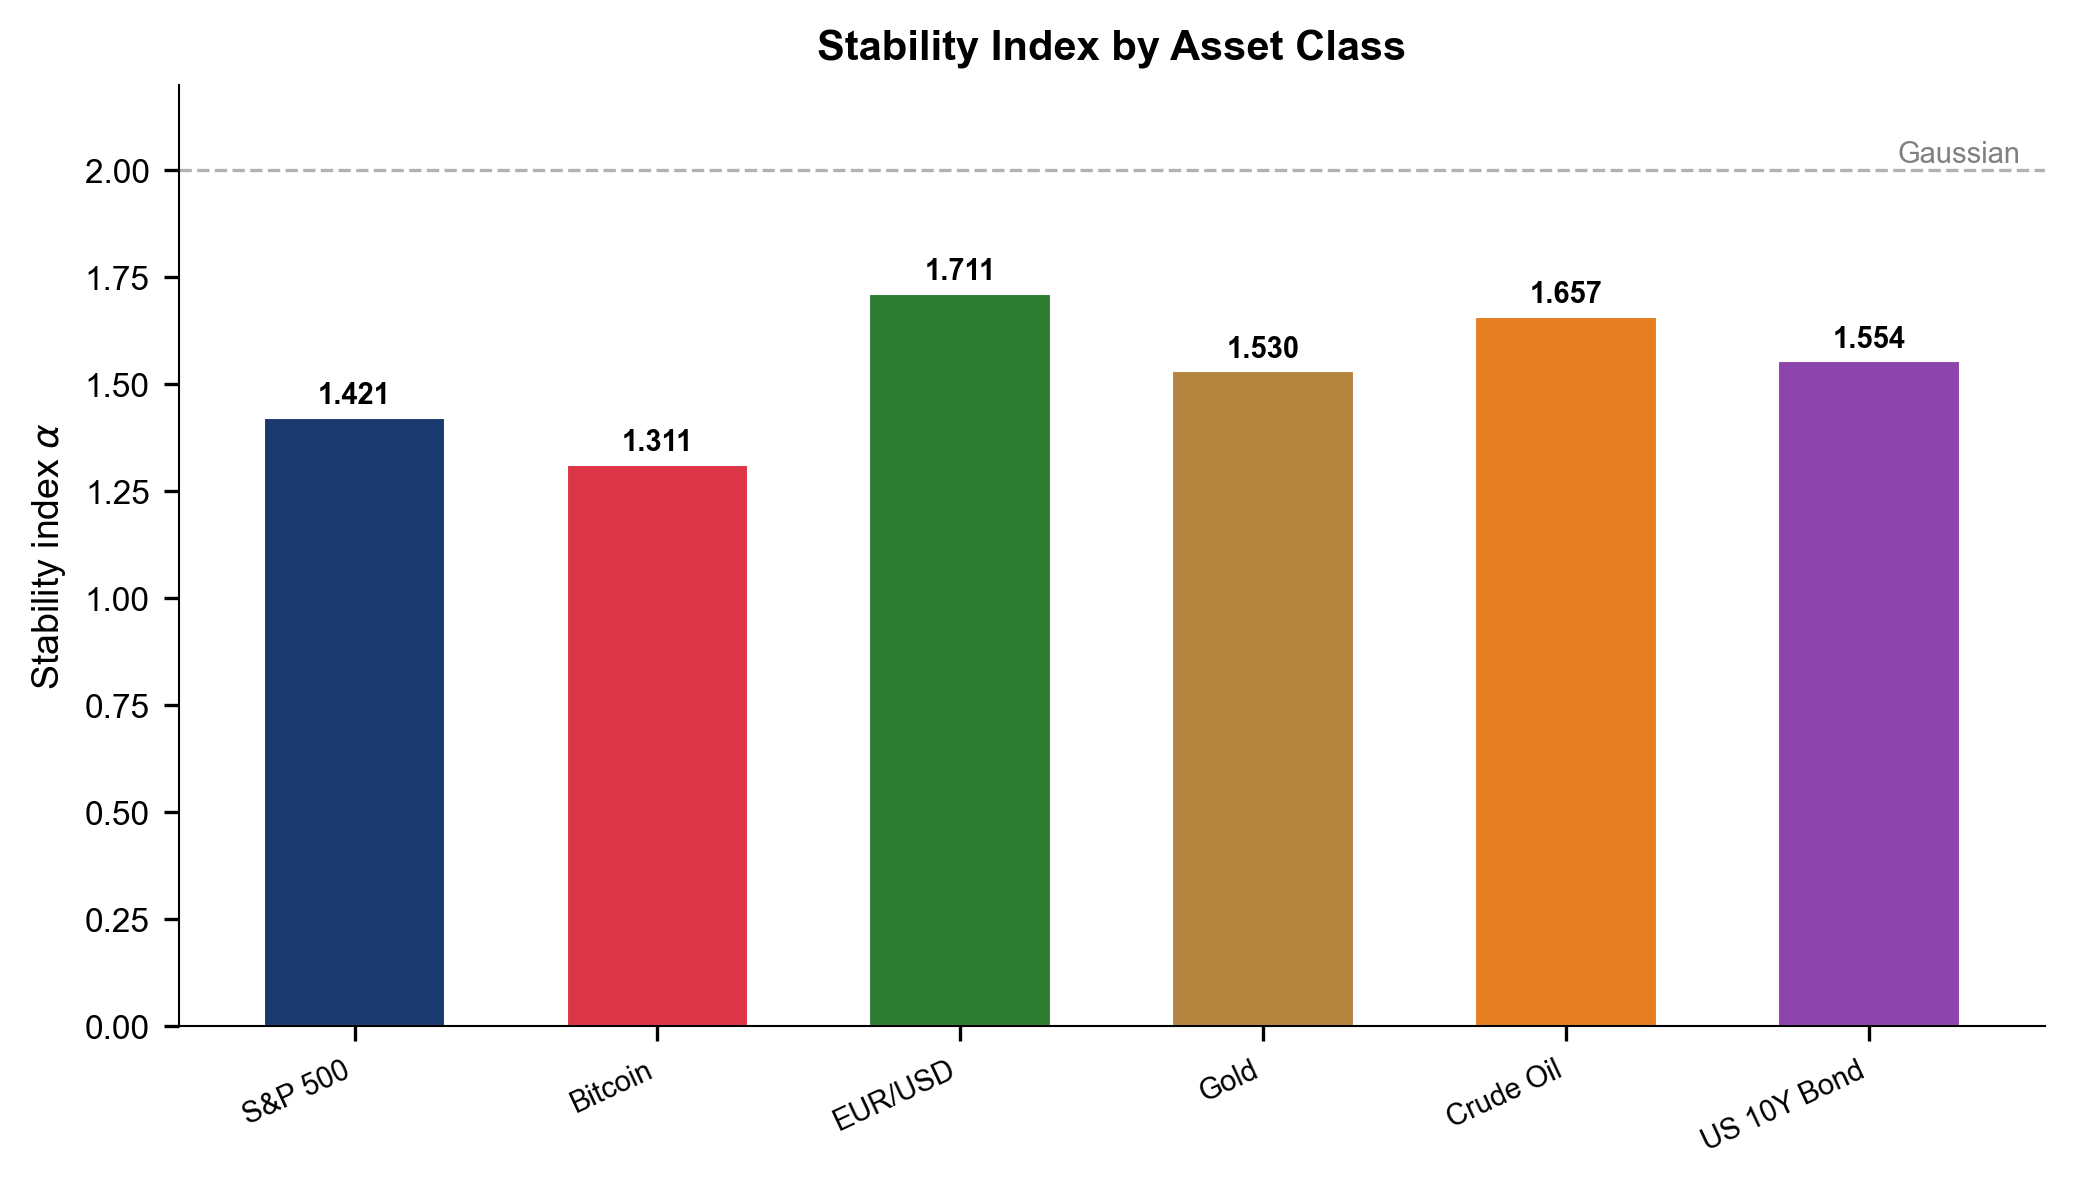
\includegraphics[width=\textwidth]{ch2_cross_asset_alpha.png}
\end{center}
\end{column}
\end{columns}

\vspace{0.2cm}
\begin{itemize}
\item $\hat{\alpha} \approx 1.7$ for S\&P~500; $\hat{\alpha} \approx 1.5$ for Bitcoin; $\hat{\alpha} \approx 1.8$ for FX
\item $\alpha < 2$ across all major asset classes $\Rightarrow$ infinite variance is ubiquitous
\end{itemize}
\end{frame}

%--- PhD Slide 9 ---
\begin{frame}{Regular Variation and Domain of Attraction}
\begin{defn}[Regular Variation]
$L : (0,\infty) \to (0,\infty)$ is \textbf{slowly varying} at infinity if $\lim_{x\to\infty} L(tx)/L(x) = 1$ for all $t > 0$. A function $f$ is \textbf{regularly varying} with index $\rho$ if $f(x) = x^\rho L(x)$.
\end{defn}

\begin{thm}[Domain of Attraction]
$F$ belongs to the domain of attraction of $S(\alpha, \beta, 1, 0)$ iff:
\begin{enumerate}
\item $\bar{F}(x) = x^{-\alpha}L(x)$ (regularly varying tails)
\item Balance condition: $\lim_{x\to\infty} \frac{\bar{F}(x)}{\bar{F}(x) + F(-x)} = \frac{1+\beta}{2}$
\end{enumerate}
\end{thm}
\end{frame}

%--- PhD Slide 10 ---
\begin{frame}{L\'{e}vy Processes}
\begin{itemize}
\item A \textbf{L\'{e}vy process} $\{L_t\}_{t\geq 0}$ has stationary independent increments
\item $L_1 \sim S(\alpha, \beta, \gamma, \delta)$ defines a \textbf{stable L\'{e}vy process}
\item \textbf{L\'{e}vy--It\^{o} decomposition}:
\[
L_t = bt + \sigma W_t + \int_{|x|\leq 1} x\,\tilde{N}(t,dx) + \int_{|x|>1} x\,N(t,dx)
\]
\item \textbf{L\'{e}vy measure} of a stable process:
\[
\nu(dx) = \begin{cases} c_+ x^{-\alpha-1}dx & x > 0 \\ c_- |x|^{-\alpha-1}dx & x < 0 \end{cases}
\]
\item Infinite activity: infinitely many small jumps in any finite interval
\end{itemize}
\end{frame}

%--- PhD Slide 11 ---
\begin{frame}{Tempered Stable Distributions}
\begin{itemize}
\item \textbf{Problem}: Pure stable distributions have infinite variance --- inconvenient for some applications
\item \textbf{Solution}: Tempered stable distributions --- modify the L\'{e}vy measure:
\[
\nu(dx) = c\,|x|^{-\alpha-1}e^{-\lambda|x|}dx
\]
\item Retain heavy-tail behavior for moderate $x$ but guarantee \textbf{finite moments}
\item Exponential tempering kills the extreme tail $\Rightarrow$ all moments exist
\item Examples: CGMY model (Carr, Geman, Madan, Yor, 2002)
\end{itemize}
\end{frame}

%--- PhD Slide 12 ---
\begin{frame}{Stable vs.\ Student-$t$: The Great Debate}
\begin{center}
\renewcommand{\arraystretch}{1.0}
\scriptsize
\begin{tabular}{lcc}
\toprule
& \textbf{Stable} & \textbf{Student-$t$} \\
\midrule
Tail index & $\alpha$ & $\nu$ \\
Finite moments & $p < \alpha$ & $p < \nu$ \\
Closed under sum & Yes & No \\
GCLT limit & Yes & No \\
Variance & $\infty$ ($\alpha < 2$) & Finite ($\nu > 2$) \\
Estimation & Harder (no closed-form PDF) & Standard MLE \\
\bottomrule
\end{tabular}
\end{center}
\begin{itemize}
\item Historical debate: Mandelbrot--Fama (stable) vs.\ Praetz--Blattberg--Gonedes (Student-$t$)
\item Modern view: both capture power-law tails; choice depends on application
\end{itemize}
\vspace{-0.2cm}
\begin{center}
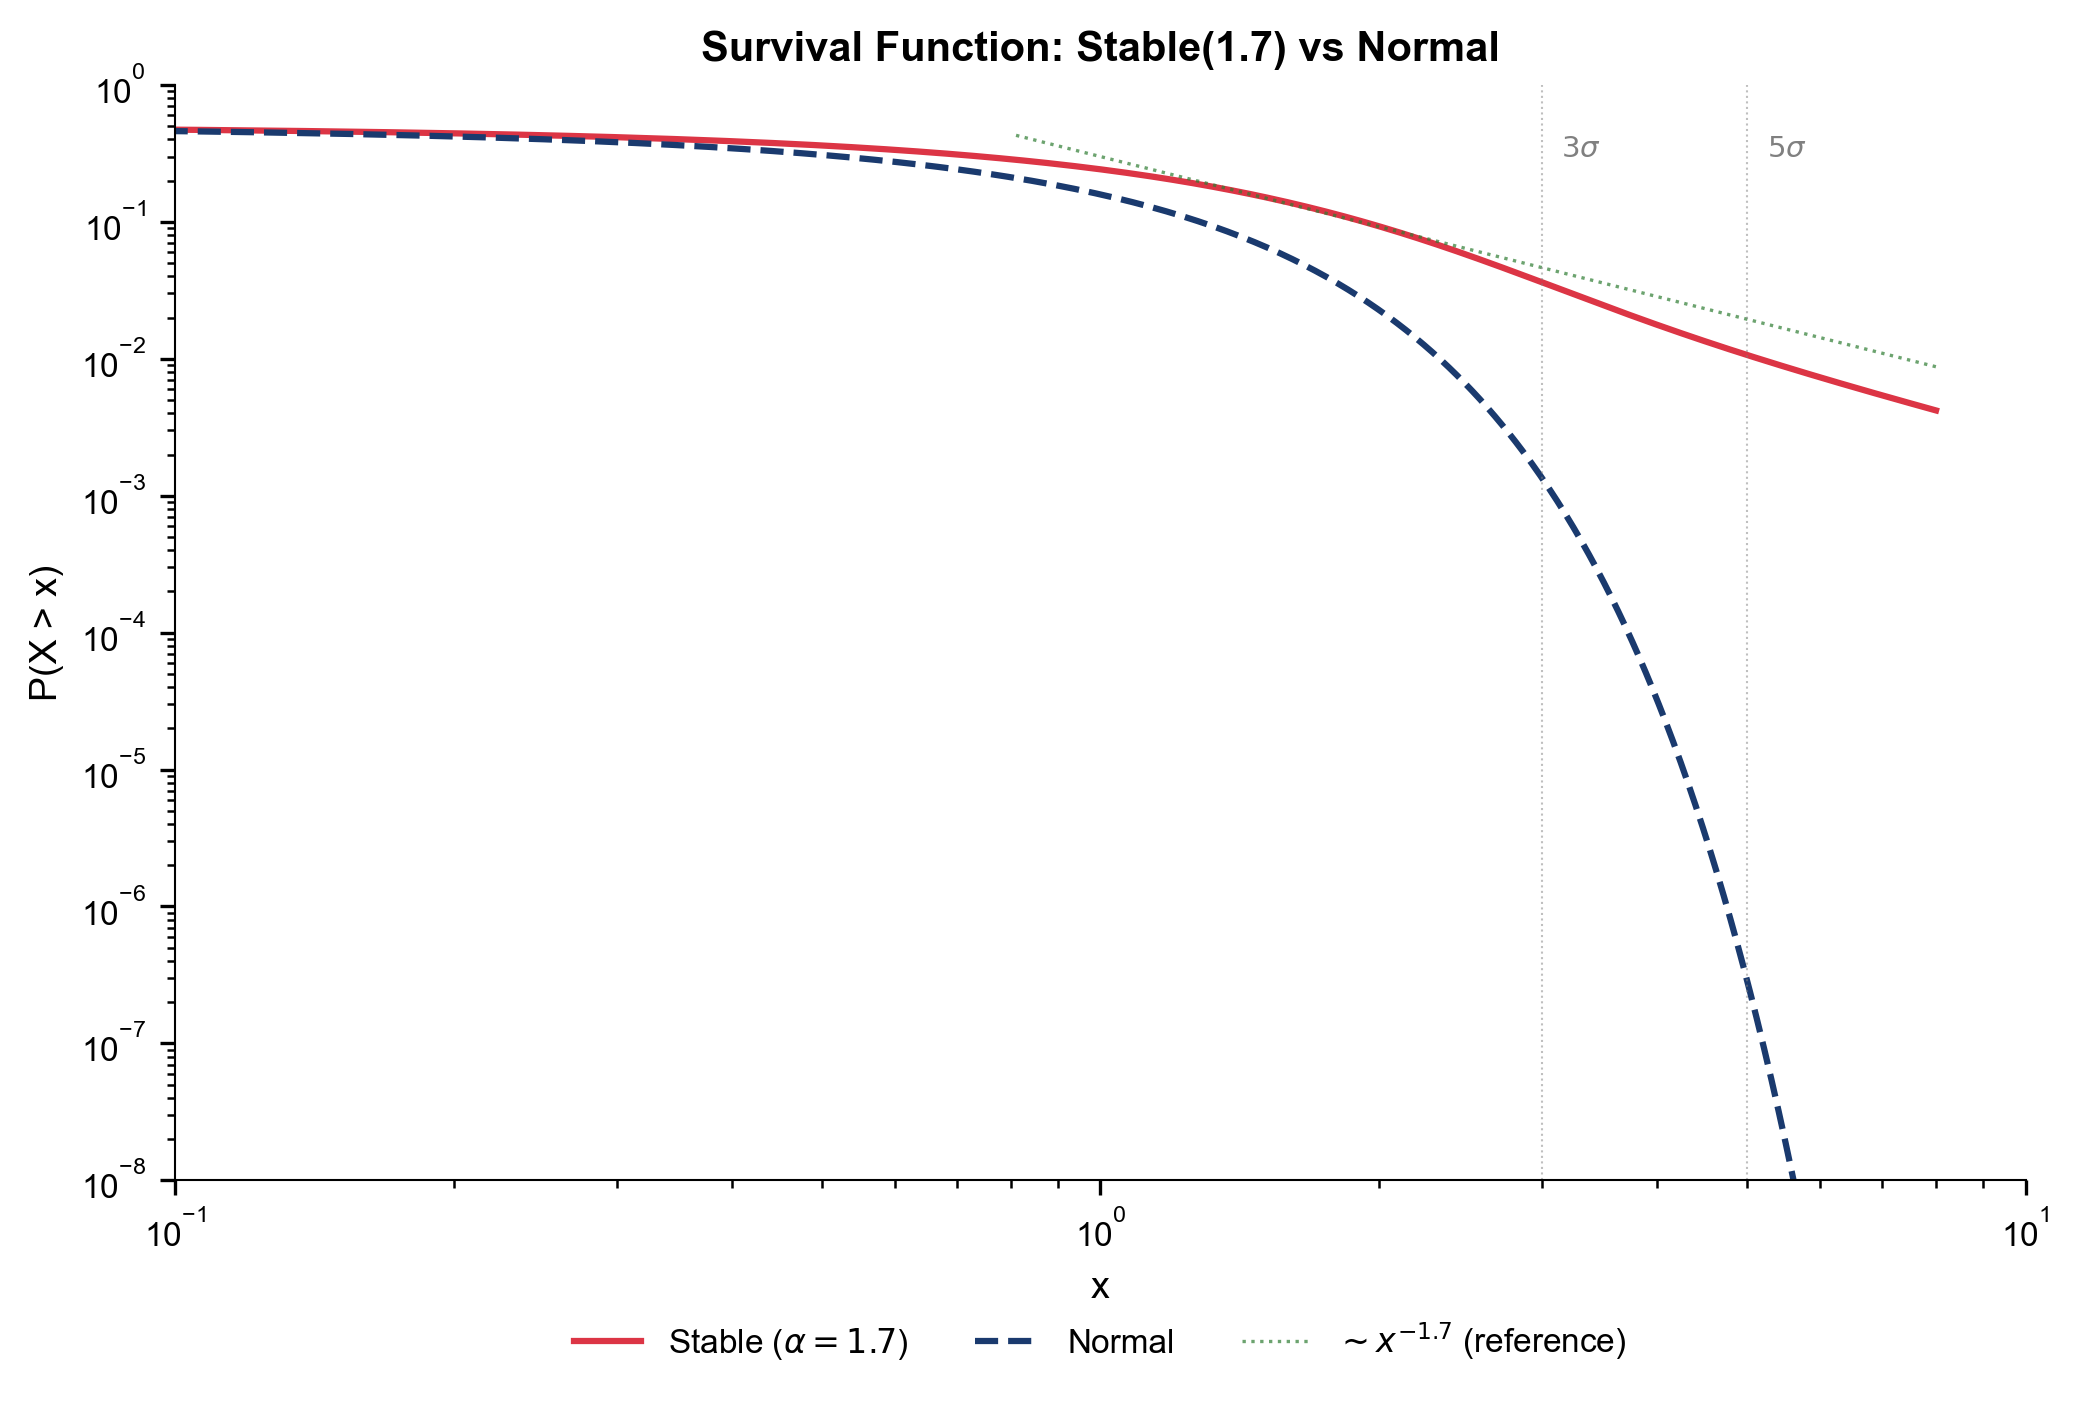
\includegraphics[height=0.22\textheight]{ch2_tail_survival.png}
\end{center}
\end{frame}

%#############################################################################
\section{Extreme Value Theory (EVT)}
%#############################################################################

%--- Y3 Slide 1 ---
\begin{frame}{EVT --- Motivation}
\begin{itemize}
\item We need accurate models for \textbf{extreme events} (financial crises, market crashes)
\item Instead of modeling the \textit{entire} distribution, EVT focuses on the \textbf{tails only}
\item \textbf{Tail index $\xi$}: a single number that summarizes tail heaviness
\begin{itemize}
\item $\xi > 0$: heavy tails (power-law decay) --- typical for financial data
\item $\xi = 0$: exponential tails (similar to Normal)
\item $\xi < 0$: bounded tails (finite maximum)
\end{itemize}
\item Financial data: $\hat{\xi} > 0$ confirms that extreme events are more frequent than the Normal predicts
\end{itemize}

\vspace{0.2cm}
\begin{block}{Key Idea}
\begin{itemize}
\item EVT provides \textbf{mathematically rigorous} extrapolation into the tails, even beyond observed data
\end{itemize}
\end{block}
\end{frame}

%--- Y3 Slide 2 ---
\begin{frame}{GPD --- Descriptive Introduction}
\begin{itemize}
\item \textbf{Exceedances} above a high threshold $u$ tend to follow a specific shape:
\[
\text{The Generalized Pareto Distribution (GPD)}
\]
\item Think of it as: ``given that something extreme happened, how extreme was it?''
\item The GPD has two parameters: shape $\xi$ and scale $\sigma$
\item For financial data, typically $\hat{\xi} \in [0.1, 0.5]$
\end{itemize}

\vspace{-0.1cm}
\begin{center}
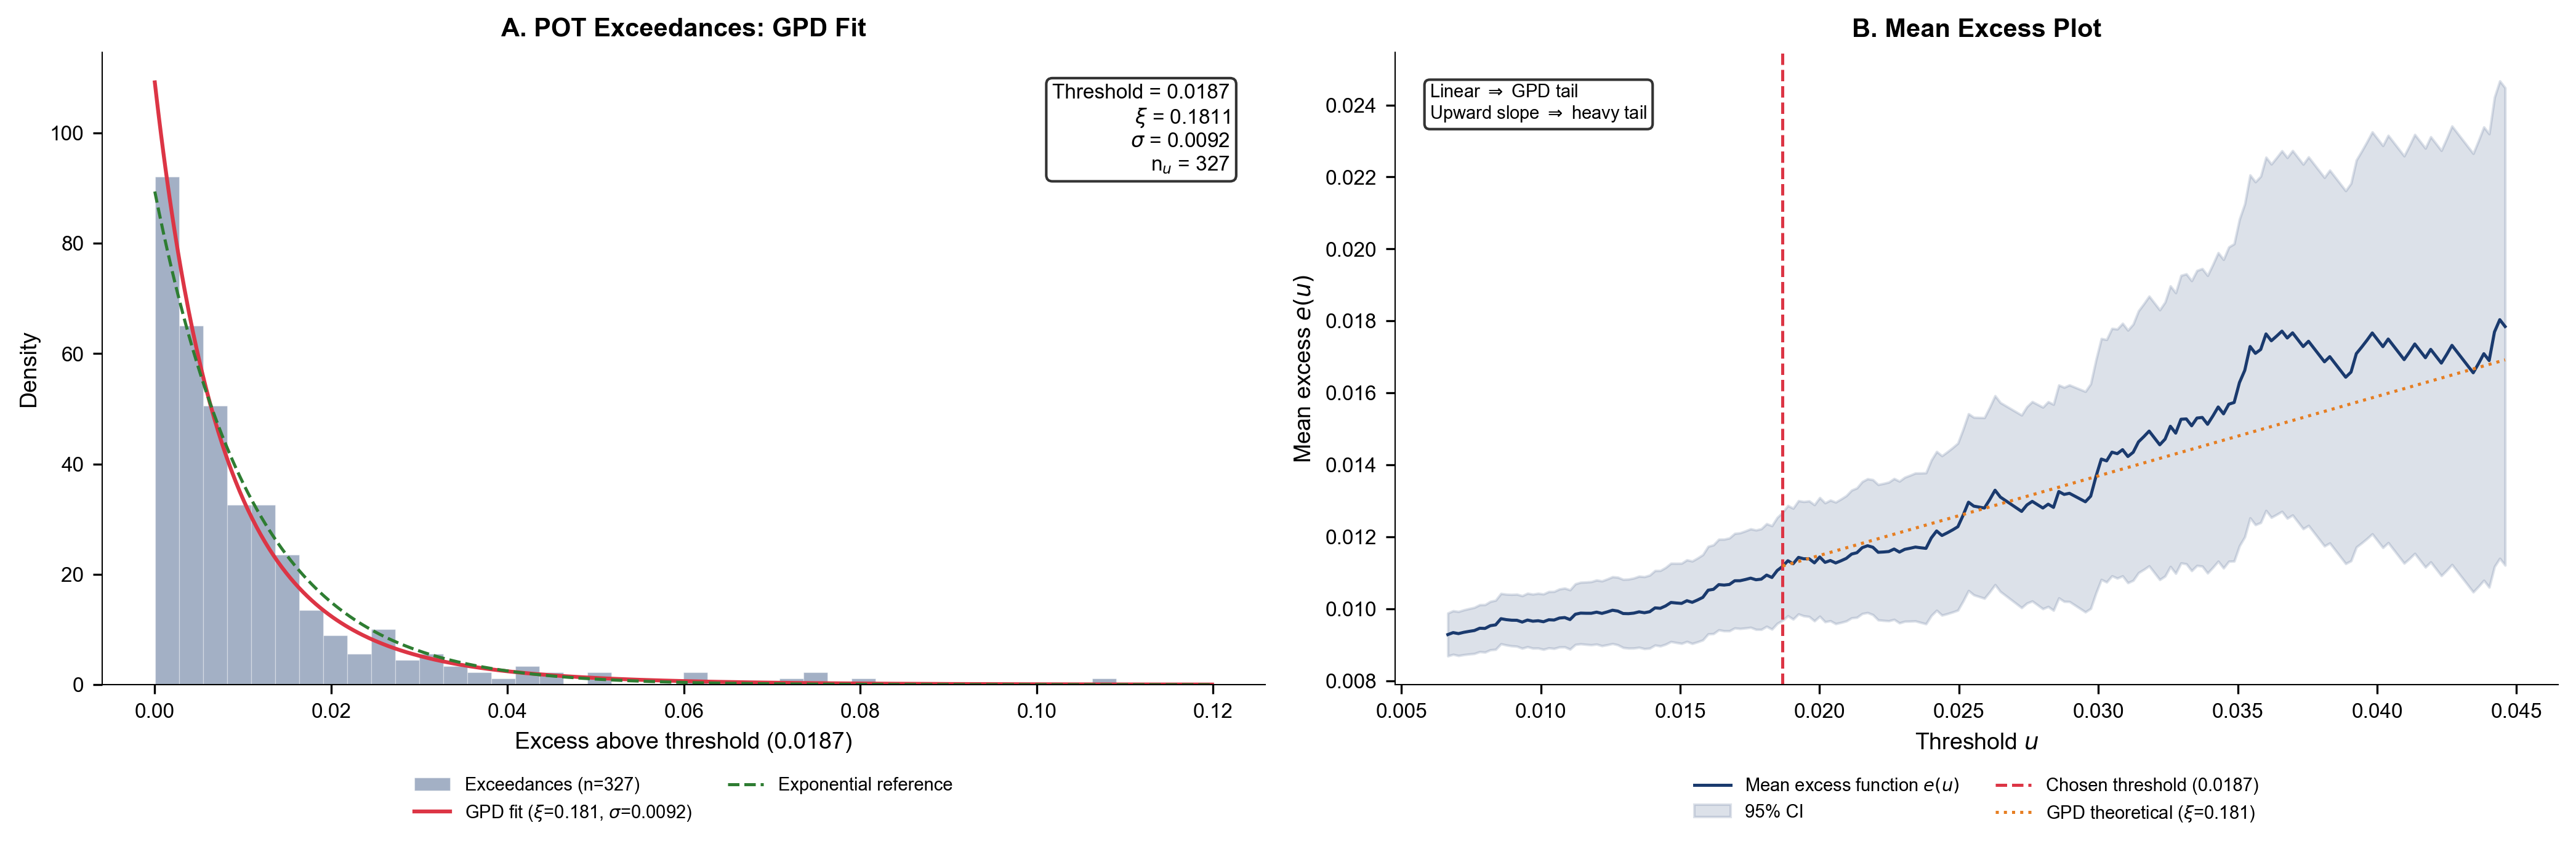
\includegraphics[width=0.50\textwidth]{ch2_evt_gpd_pot.png}
\end{center}
\end{frame}

%--- Y3 Slide 3 ---
\begin{frame}{EVT in Practice --- Extreme Events}
\begin{center}
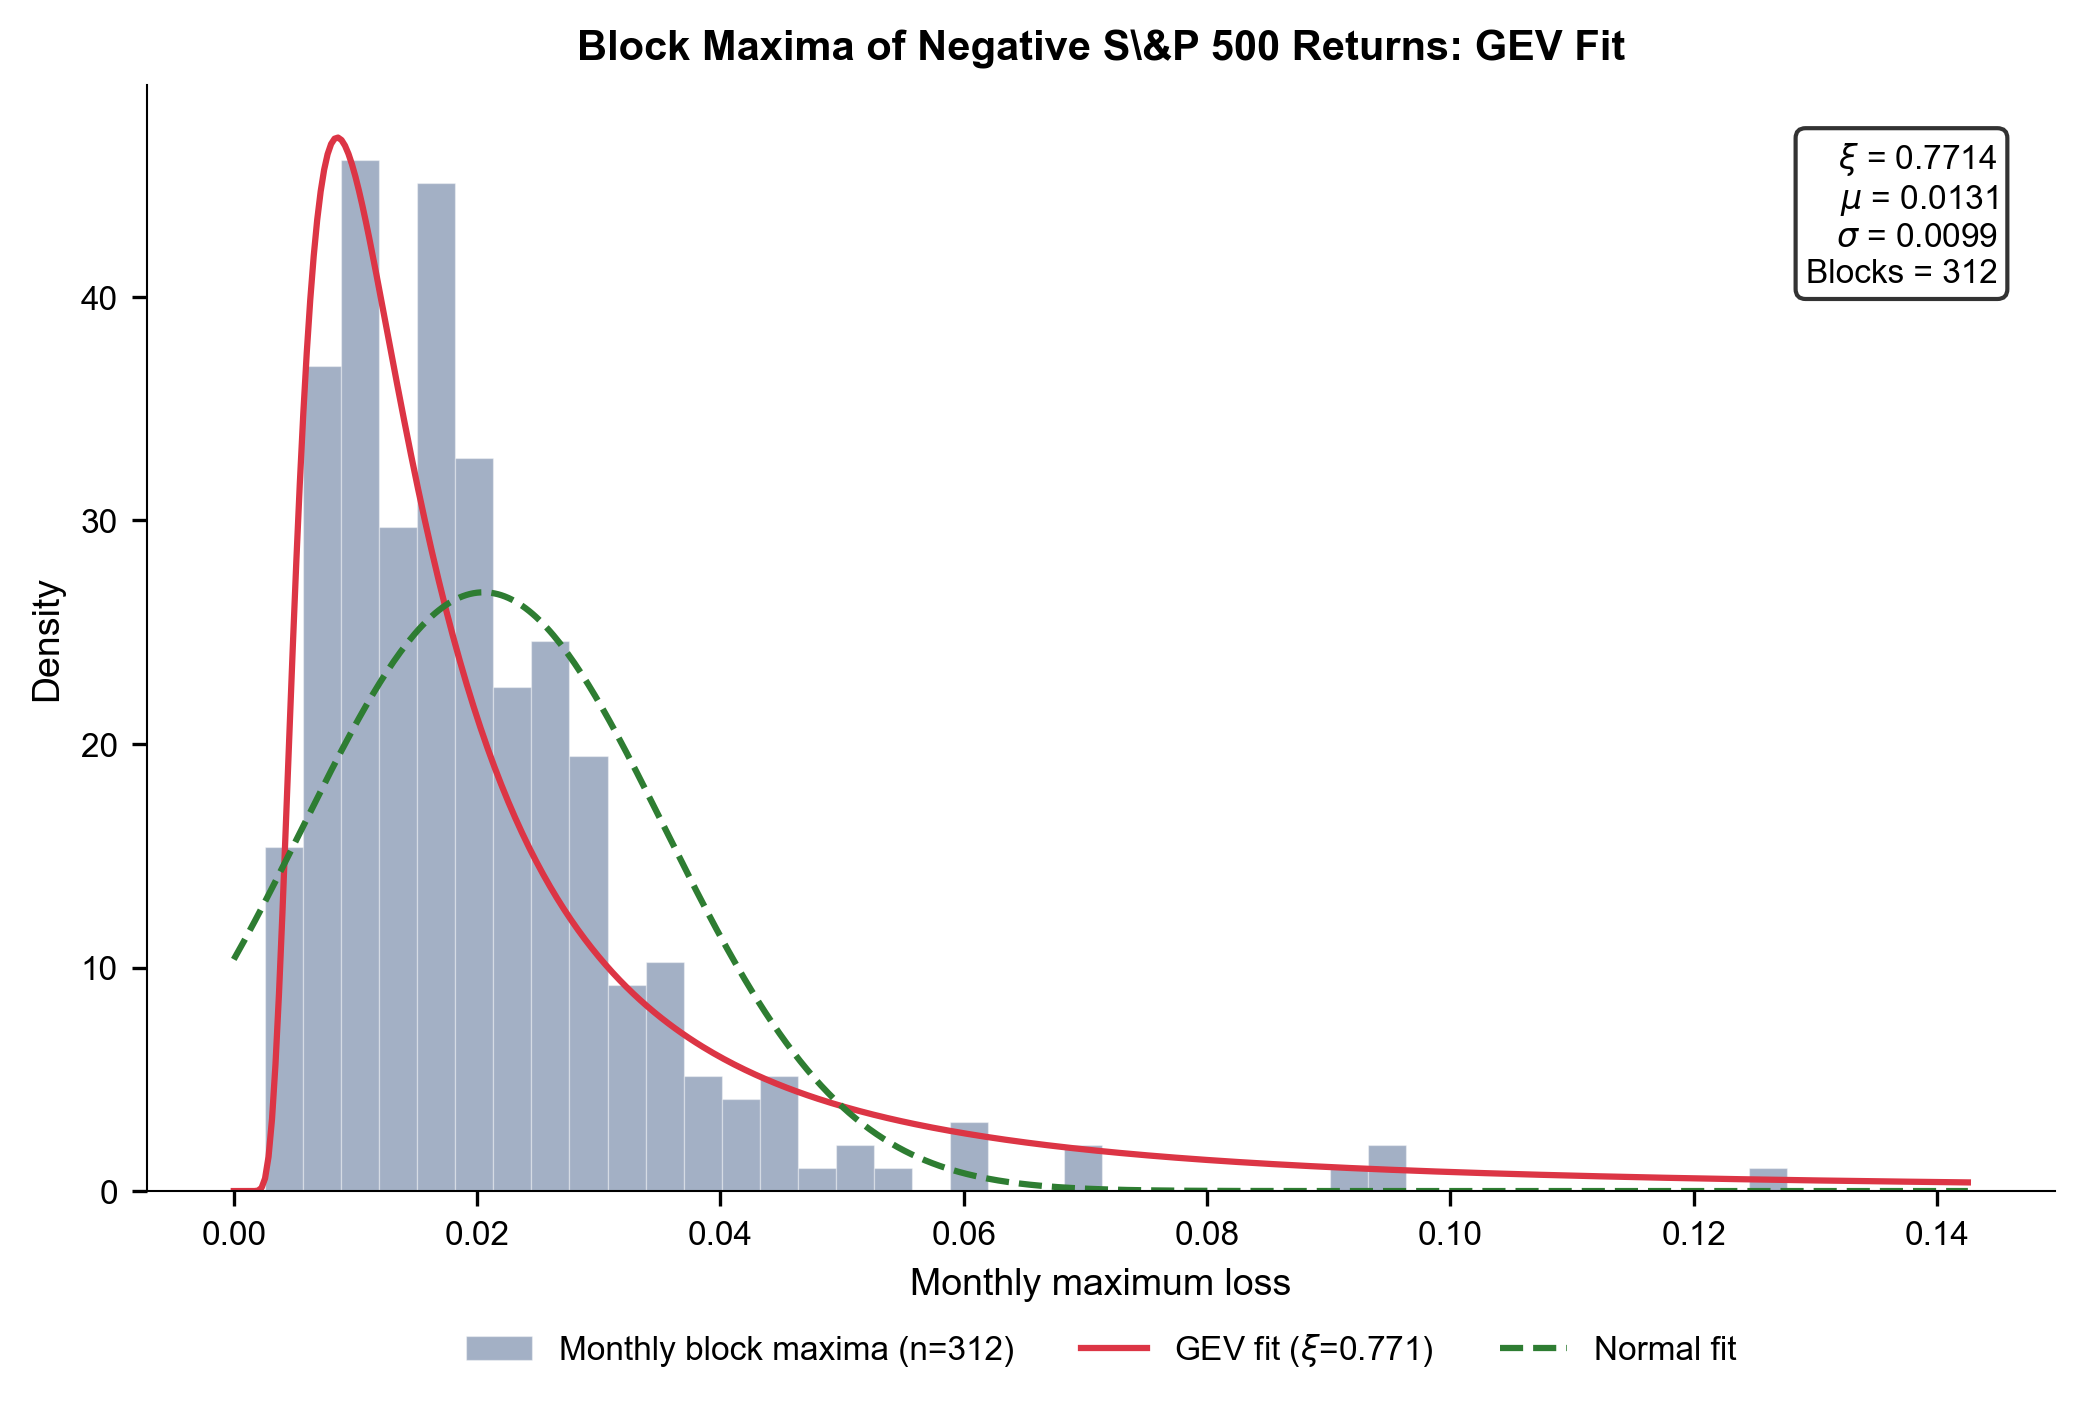
\includegraphics[width=0.55\textwidth]{ch2_evt_gev_fit.png}
\end{center}
\begin{itemize}
\item Block maxima (e.g., monthly worst loss) follow the GEV distribution
\item Formal theorems at Master level; EVT-based VaR/ES in Section~2.10
\end{itemize}
\end{frame}

%--- MSc Slide 4 ---
\begin{frame}{Fisher--Tippett--Gnedenko Theorem}
\begin{thm}[Fisher--Tippett--Gnedenko]
If $M_n = \max(X_1, \ldots, X_n)$ and $\frac{M_n - b_n}{a_n} \xrightarrow{d} H$, then $H$ is the \textbf{GEV}:
\[
H(x;\xi,\mu,\sigma) = \exp\!\left\{-\left(1 + \xi\frac{x-\mu}{\sigma}\right)^{-1/\xi}\right\}
\]
\end{thm}

\begin{itemize}
\item Three types depending on $\xi$:
\begin{itemize}
\item $\xi > 0$: \textbf{Fr\'{e}chet} --- heavy tails (financial data)
\item $\xi = 0$: \textbf{Gumbel} --- exponential tails
\item $\xi < 0$: \textbf{Weibull} --- bounded tails
\end{itemize}
\item Analogous to CLT but for \textit{maxima} instead of sums
\end{itemize}
\end{frame}

%--- MSc Slide 5 ---
\begin{frame}{Pickands--Balkema--de Haan and POT Method}
\begin{thm}[Pickands--Balkema--de Haan]
For high threshold $u$, exceedances $Y = X - u \mid X > u$ follow the GPD:
\[
G(y;\xi,\sigma) = 1 - \left(1 + \xi\frac{y}{\sigma}\right)^{-1/\xi}, \quad y > 0.
\]
\end{thm}

\begin{itemize}
\item \textbf{POT method} (Peaks Over Threshold):
\begin{enumerate}
\item Choose threshold $u$ (mean excess plot, parameter stability)
\item Fit GPD to exceedances via MLE
\item Report $(\hat{\xi}, \hat{\sigma})$
\end{enumerate}
\item \textbf{Mean excess function}: $e(u) = \E[X - u \mid X > u] = \frac{\sigma + \xi u}{1 - \xi}$
\item Linear in $u$ for GPD $\Rightarrow$ diagnostic tool for threshold selection
\end{itemize}
\end{frame}

%--- MSc Slide 6 ---
\begin{frame}{EVT-Based VaR and ES}
\begin{itemize}
\item \textbf{VaR from GPD}:
\[
\text{VaR}_\alpha = u + \frac{\sigma}{\xi}\!\left[\left(\frac{n\alpha}{N_u}\right)^{-\xi} - 1\right]
\]
where $N_u$ = number of exceedances, $n$ = total observations
\item \textbf{ES from GPD}: $\text{ES}_\alpha = \frac{\text{VaR}_\alpha}{1-\xi} + \frac{\sigma - \xi u}{1-\xi}$, \quad $\xi < 1$
\end{itemize}

\vspace{0.2cm}
\begin{center}
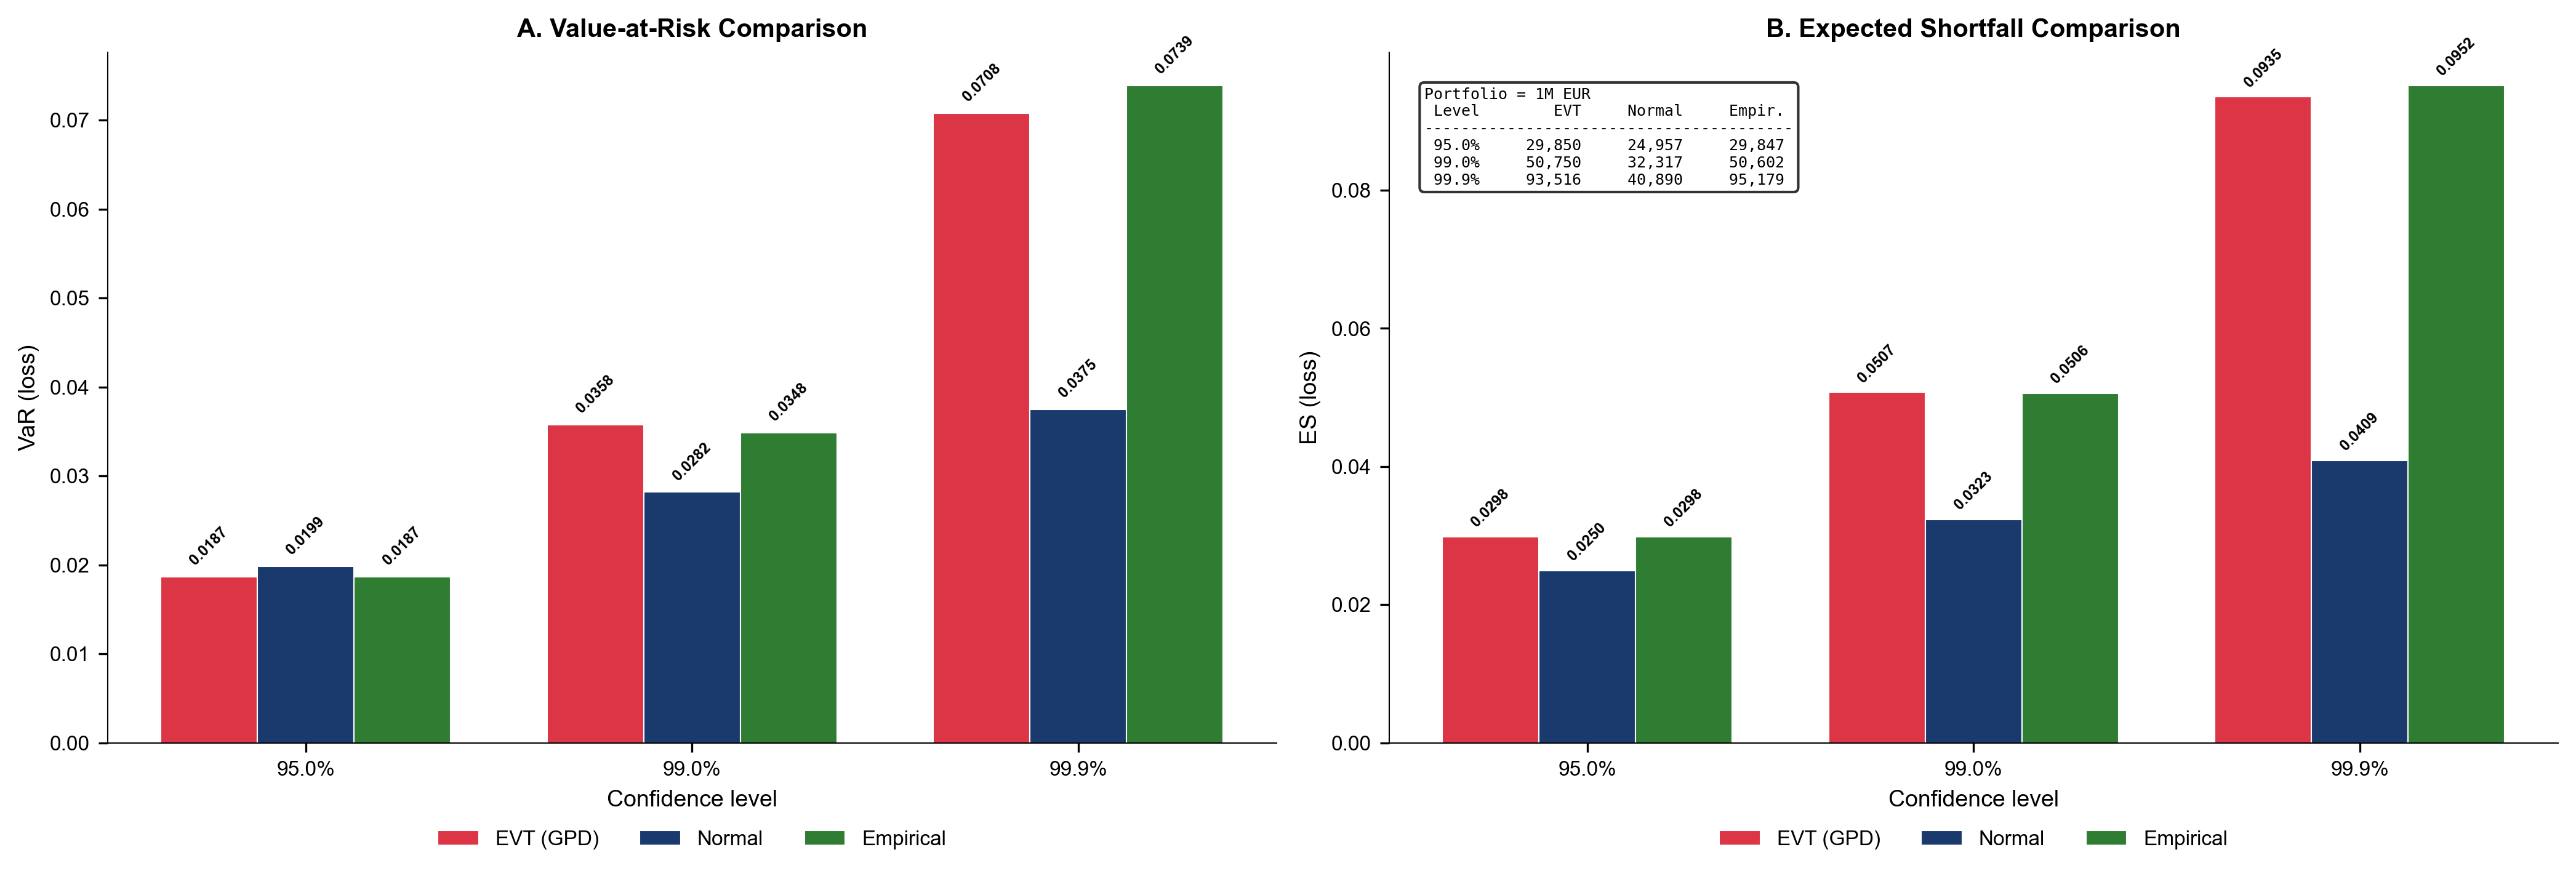
\includegraphics[width=0.6\textwidth]{ch2_evt_var_es.png}
\end{center}
\end{frame}

%--- MSc Slide 7 ---
\begin{frame}{Threshold Selection}
\begin{itemize}
\item \textbf{Mean excess plot}: plot $\hat{e}(u)$ vs.\ $u$; linearity suggests GPD is appropriate above that $u$
\item \textbf{Parameter stability plot}: $\hat{\xi}(u)$ and $\hat{\sigma}^*(u)$ vs.\ $u$; stable region = good threshold
\item Trade-off: too low $u$ $\Rightarrow$ bias (non-tail data included); too high $u$ $\Rightarrow$ high variance (few exceedances)
\item Rule of thumb: use the top 5--10\% of observations
\end{itemize}
\end{frame}

%--- PhD Slide 8 ---
\begin{frame}{Hill Estimator}
\begin{defn}[Hill Estimator]
For order statistics $X_{(1)} \geq X_{(2)} \geq \cdots \geq X_{(n)}$:
\[
\hat{\xi}_{\text{Hill}}^{(k)} = \frac{1}{k}\sum_{i=1}^{k}\ln X_{(i)} - \ln X_{(k+1)}, \quad k = 1, \ldots, n-1.
\]
The tail index is $\alpha = 1/\hat{\xi}_{\text{Hill}}$.
\end{defn}

\begin{itemize}
\item \textbf{Hill plot}: $\hat{\xi}_{\text{Hill}}^{(k)}$ vs.\ $k$; stable region indicates appropriate $k$
\item \textbf{Bias--variance trade-off}: small $k$ $\Rightarrow$ high variance; large $k$ $\Rightarrow$ high bias
\item Only valid for $\xi > 0$ (heavy tails)
\end{itemize}
\end{frame}

%--- PhD Slide 9 ---
\begin{frame}{Alternative Tail Index Estimators}
\begin{itemize}
\item \textbf{Pickands estimator}:
\[
\hat{\xi} = \frac{1}{\ln 2}\ln\frac{X_{(k)} - X_{(2k)}}{X_{(2k)} - X_{(4k)}}
\]
Works for all $\xi \in \R$ (not just $\xi > 0$)
\item \textbf{Moment estimator} (Dekkers--Einmahl--de Haan): also works for all $\xi$
\item \textbf{Second-order conditions}: Hall (1982) --- second-order parameter $\rho$ governs optimal $k$ in Hill estimator
\item \textbf{Adaptive threshold selection}: minimize asymptotic MSE (Danielsson et al., 2001)
\end{itemize}
\end{frame}

%--- PhD Slide 10 ---
\begin{frame}{Connection to Stable Distributions}
\begin{itemize}
\item If $X \sim S(\alpha, \beta, \gamma, \delta)$ with $\alpha < 2$, then the EVT shape parameter is:
\[
\xi = 1/\alpha
\]
\item Stable distributions are in the domain of attraction of the Fr\'{e}chet GEV ($\xi > 0$)
\item Hill estimator applied to stable data: $\hat{\alpha}_{\text{Hill}} = 1/\hat{\xi}_{\text{Hill}}$
\item Comparing tail indices:
\begin{itemize}
\item Stable fit: $\hat{\alpha} \approx 1.7$ $\Rightarrow$ $\hat{\xi} \approx 0.59$
\item Hill estimate: typically gives $\hat{\alpha} \in [3, 5]$ (for moderate tails)
\item The discrepancy arises because Hill measures the \textit{local} tail decay, while stable $\alpha$ governs the \textit{global} shape
\end{itemize}
\end{itemize}
\end{frame}

%#############################################################################
\section{Distribution Comparison and Model Selection}
%#############################################################################

%--- Y3 Slide 1 ---
\begin{frame}{Visual Comparison of Distributions}
\quantlet{SFM\_ch2\_dist\_comparison}{https://github.com/QuantLet/SFM/tree/master/QID-3447-SFMdist}
\begin{center}
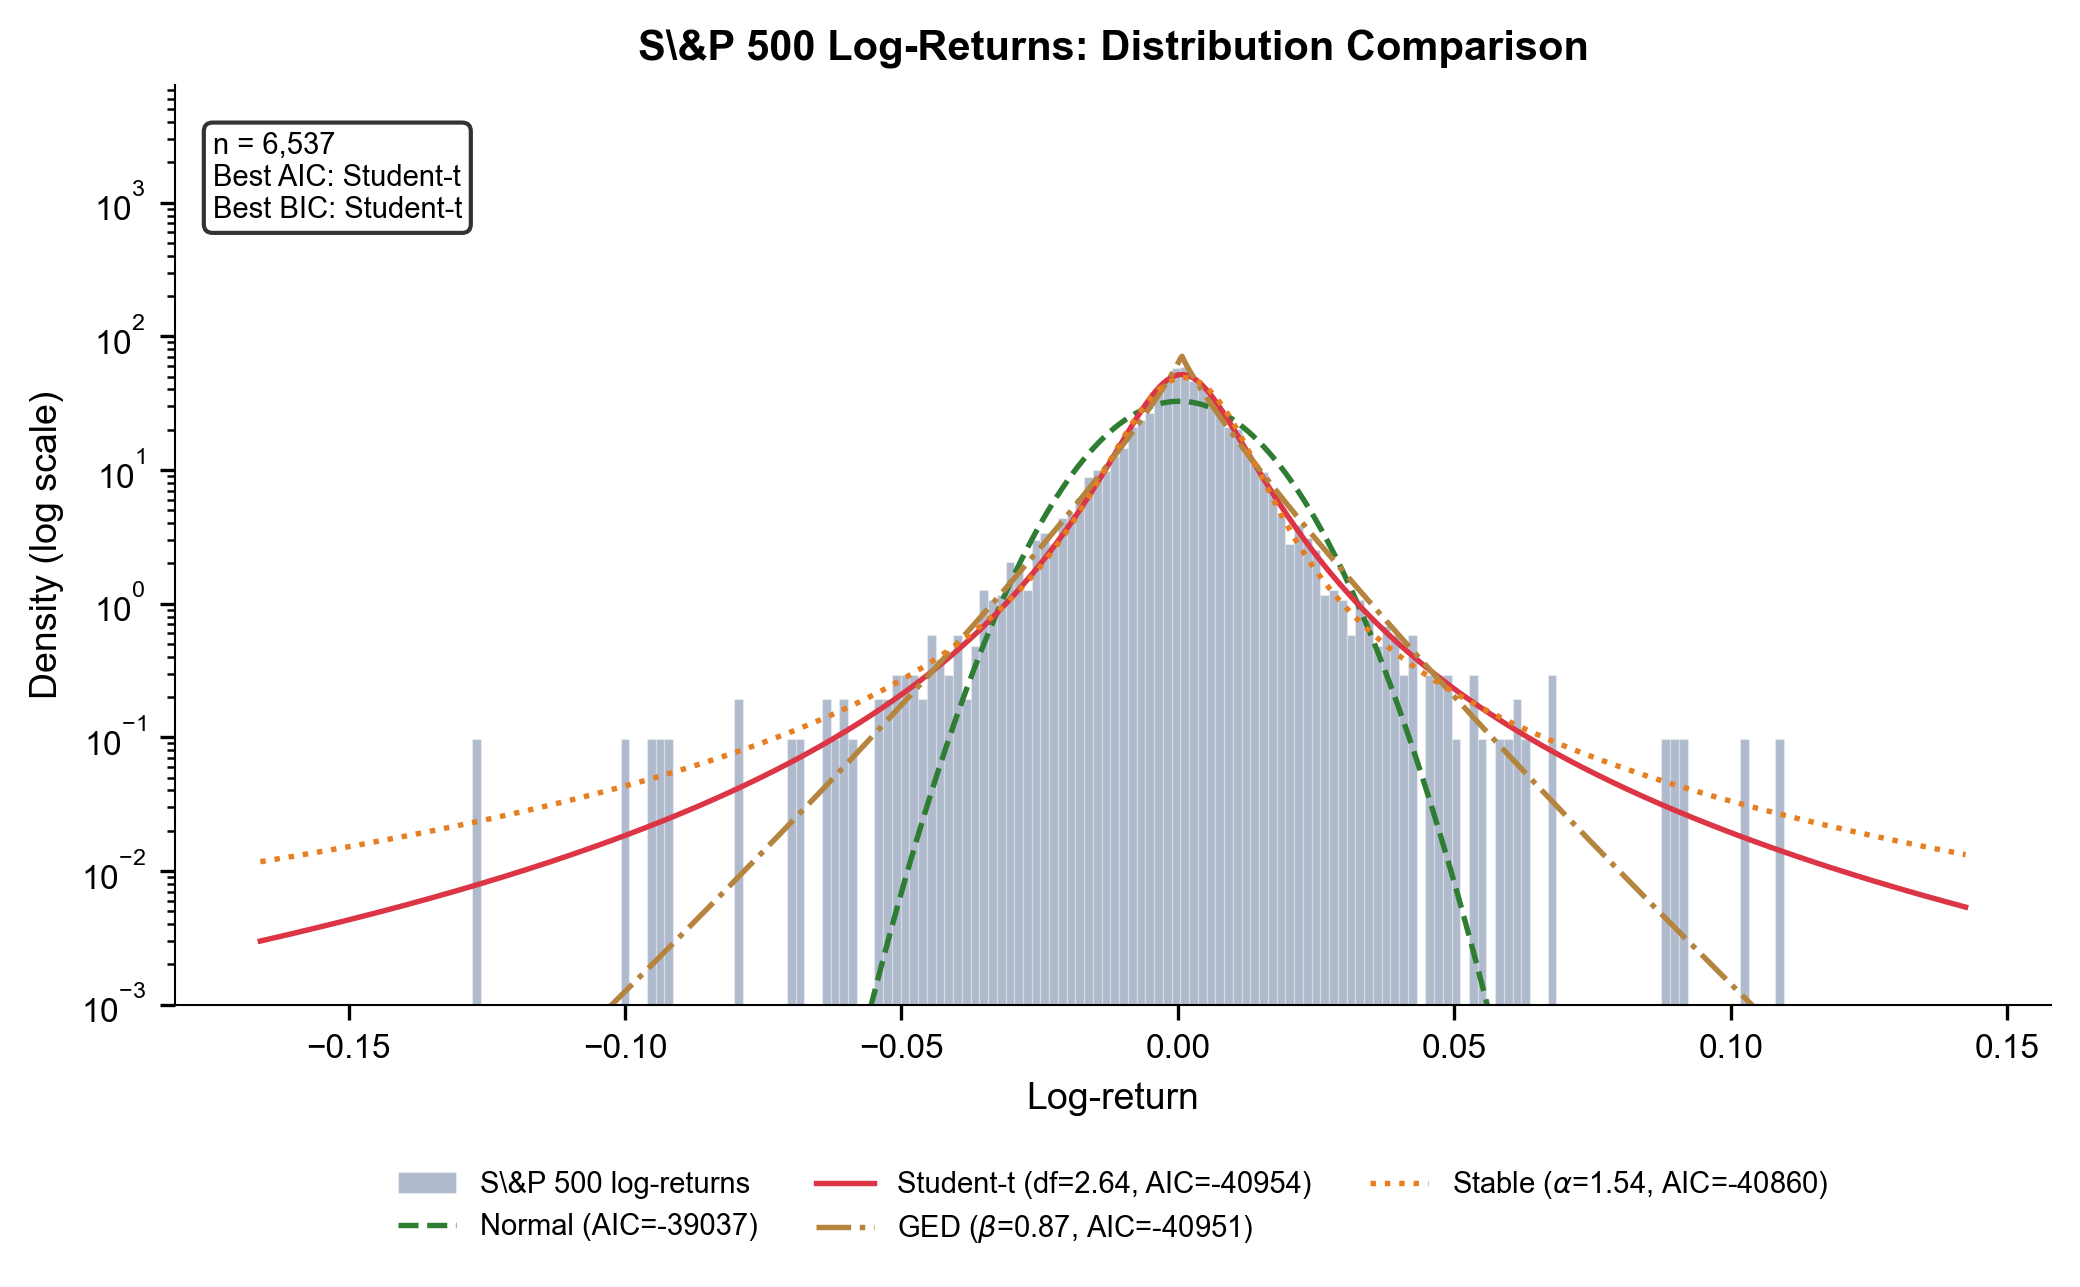
\includegraphics[width=0.5\textwidth]{ch2_dist_comparison_overlay.png}
\end{center}
\begin{itemize}
\item Histogram with fitted overlays: Normal, Student-$t$, Stable
\item Which distribution best captures the center, shoulders, and tails?
\end{itemize}
\end{frame}

%--- Y3 Slide 2 ---
\begin{frame}{QQ-Plots}
\begin{columns}[T]
\begin{column}{0.48\textwidth}
\begin{center}
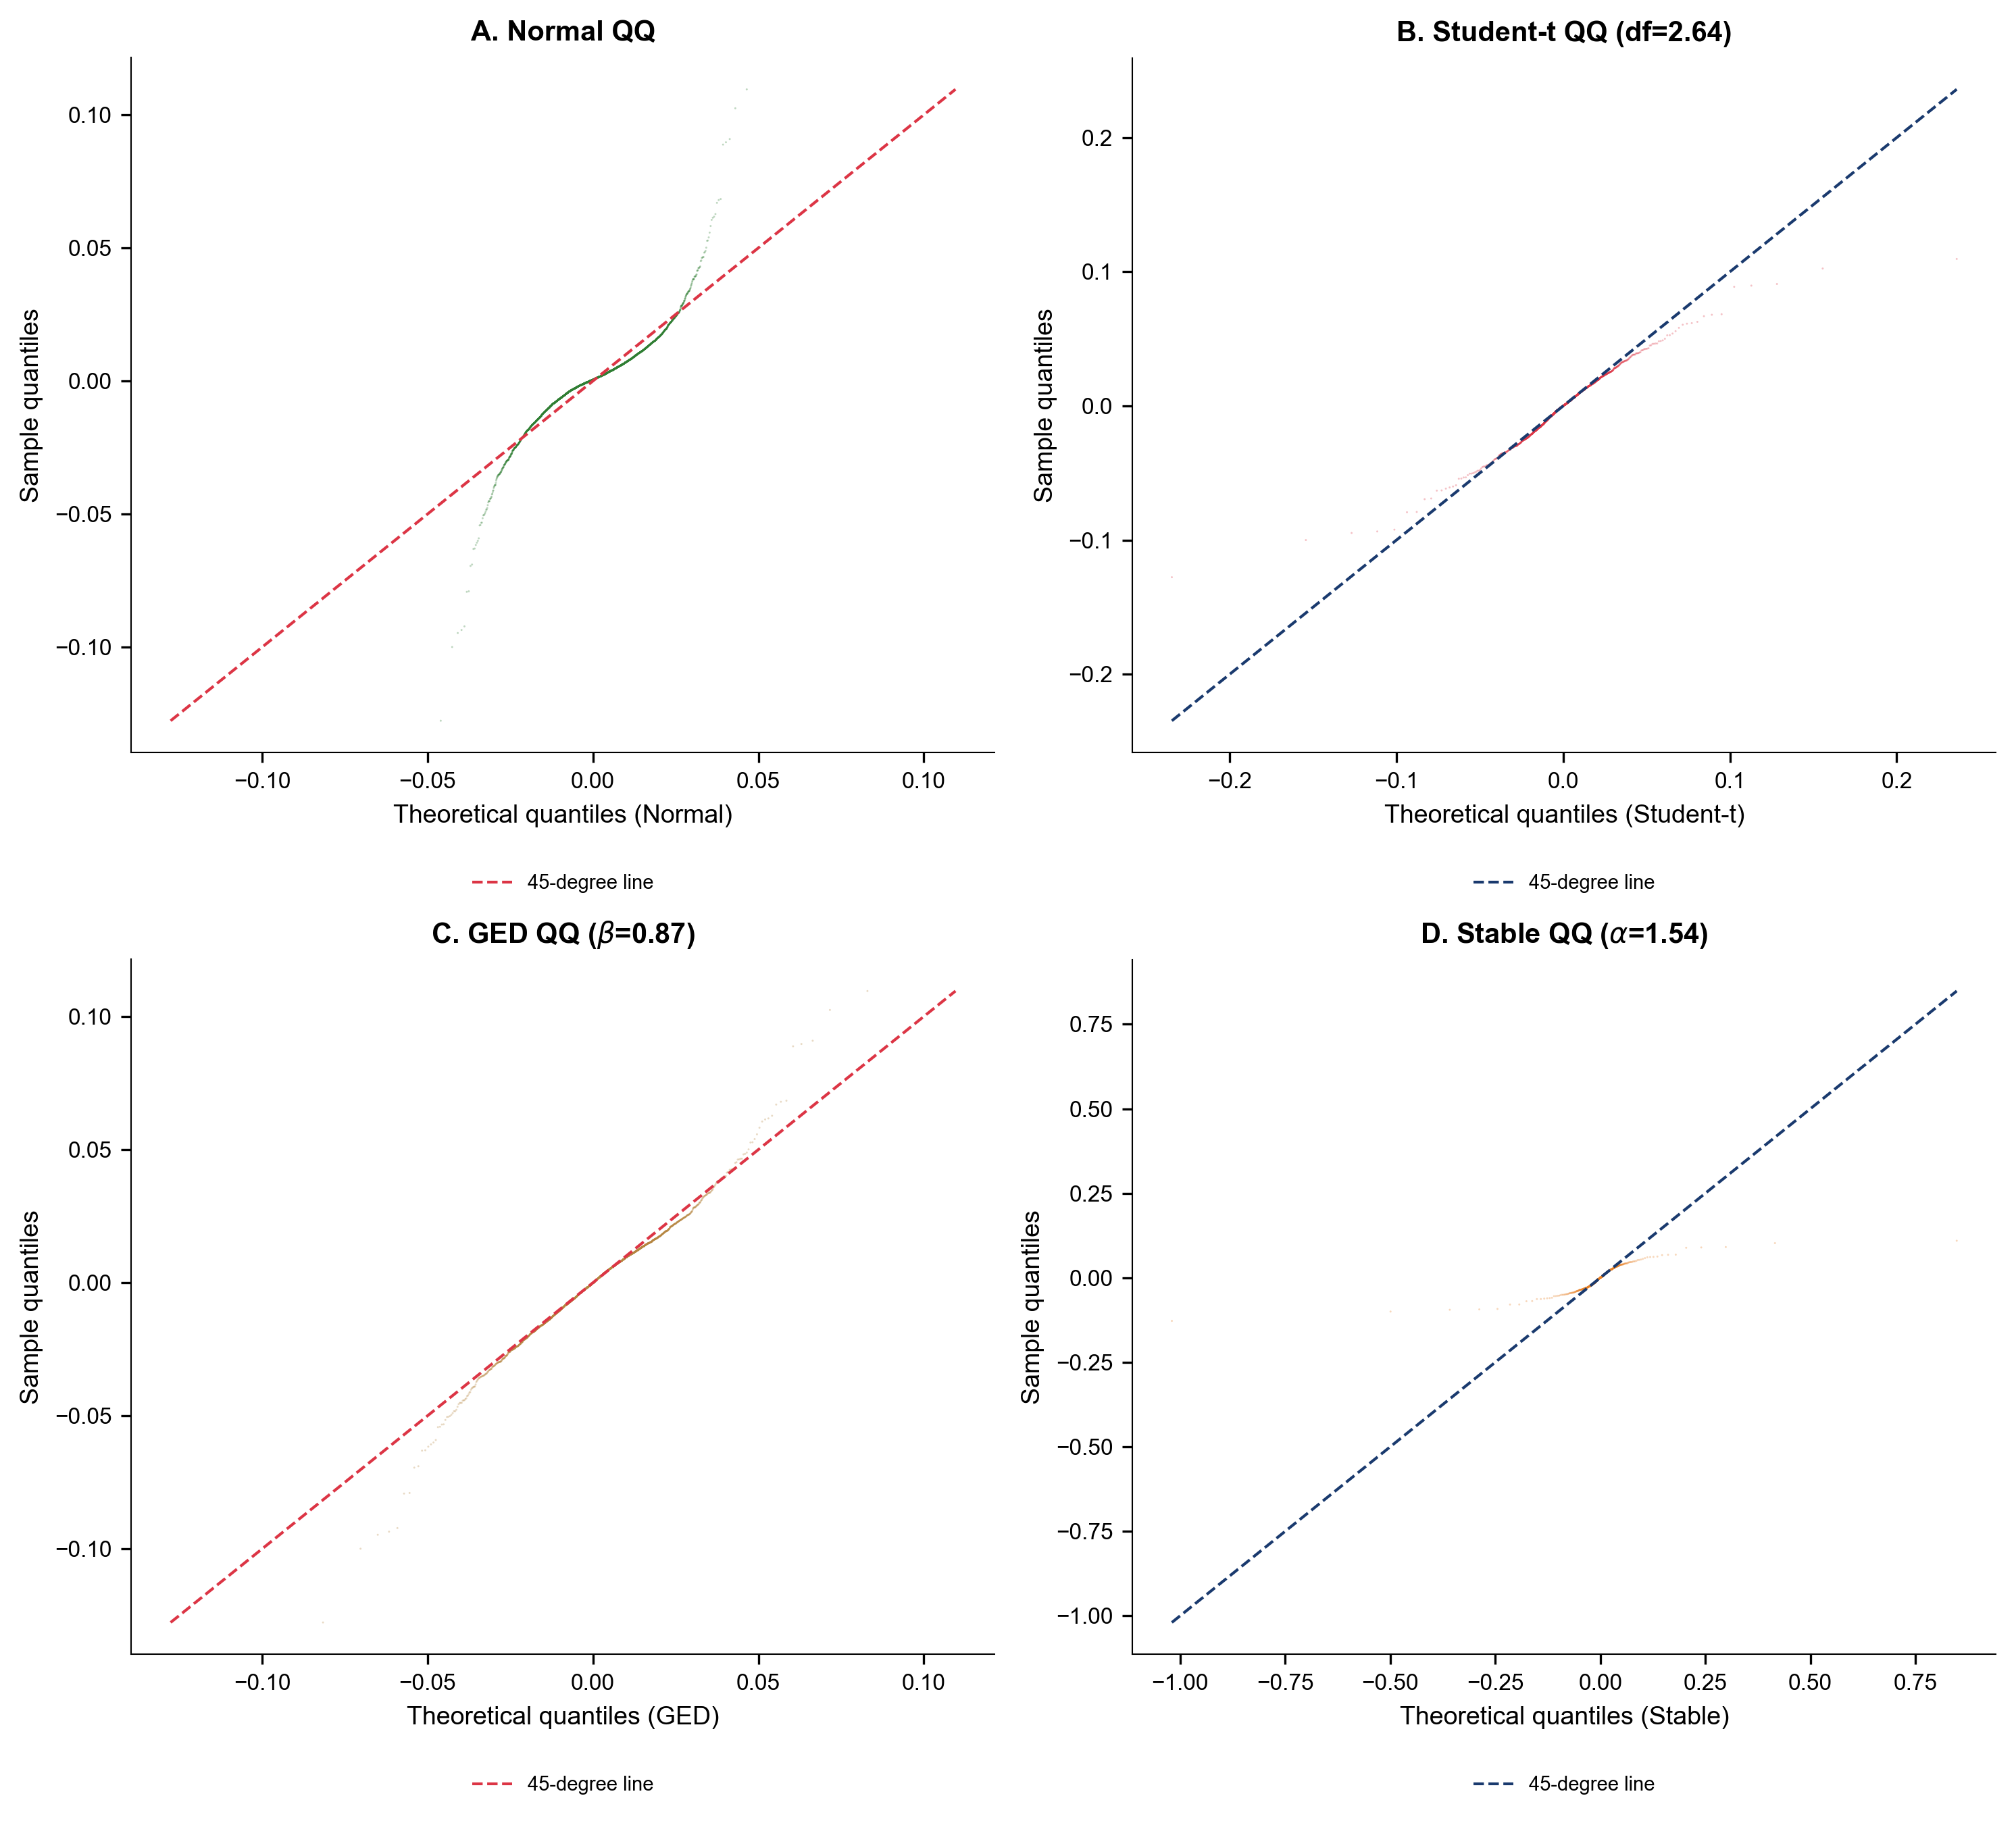
\includegraphics[width=0.95\textwidth]{ch2_dist_comparison_qq.png}
\end{center}
\end{column}
\begin{column}{0.48\textwidth}
\begin{itemize}
\item \textbf{QQ-plot}: Quantiles of data vs.\ theoretical distribution
\item Perfect fit $\Rightarrow$ points on 45$^\circ$ line
\item \textbf{S-shape}: heavier tails than model
\item Normal QQ: systematic tail deviations
\item Student-$t$ QQ: closer to 45$^\circ$ line
\end{itemize}
\end{column}
\end{columns}
\end{frame}

%--- Y3 Slide 3 ---
\begin{frame}{Log-Log Tail Plot}
\begin{center}
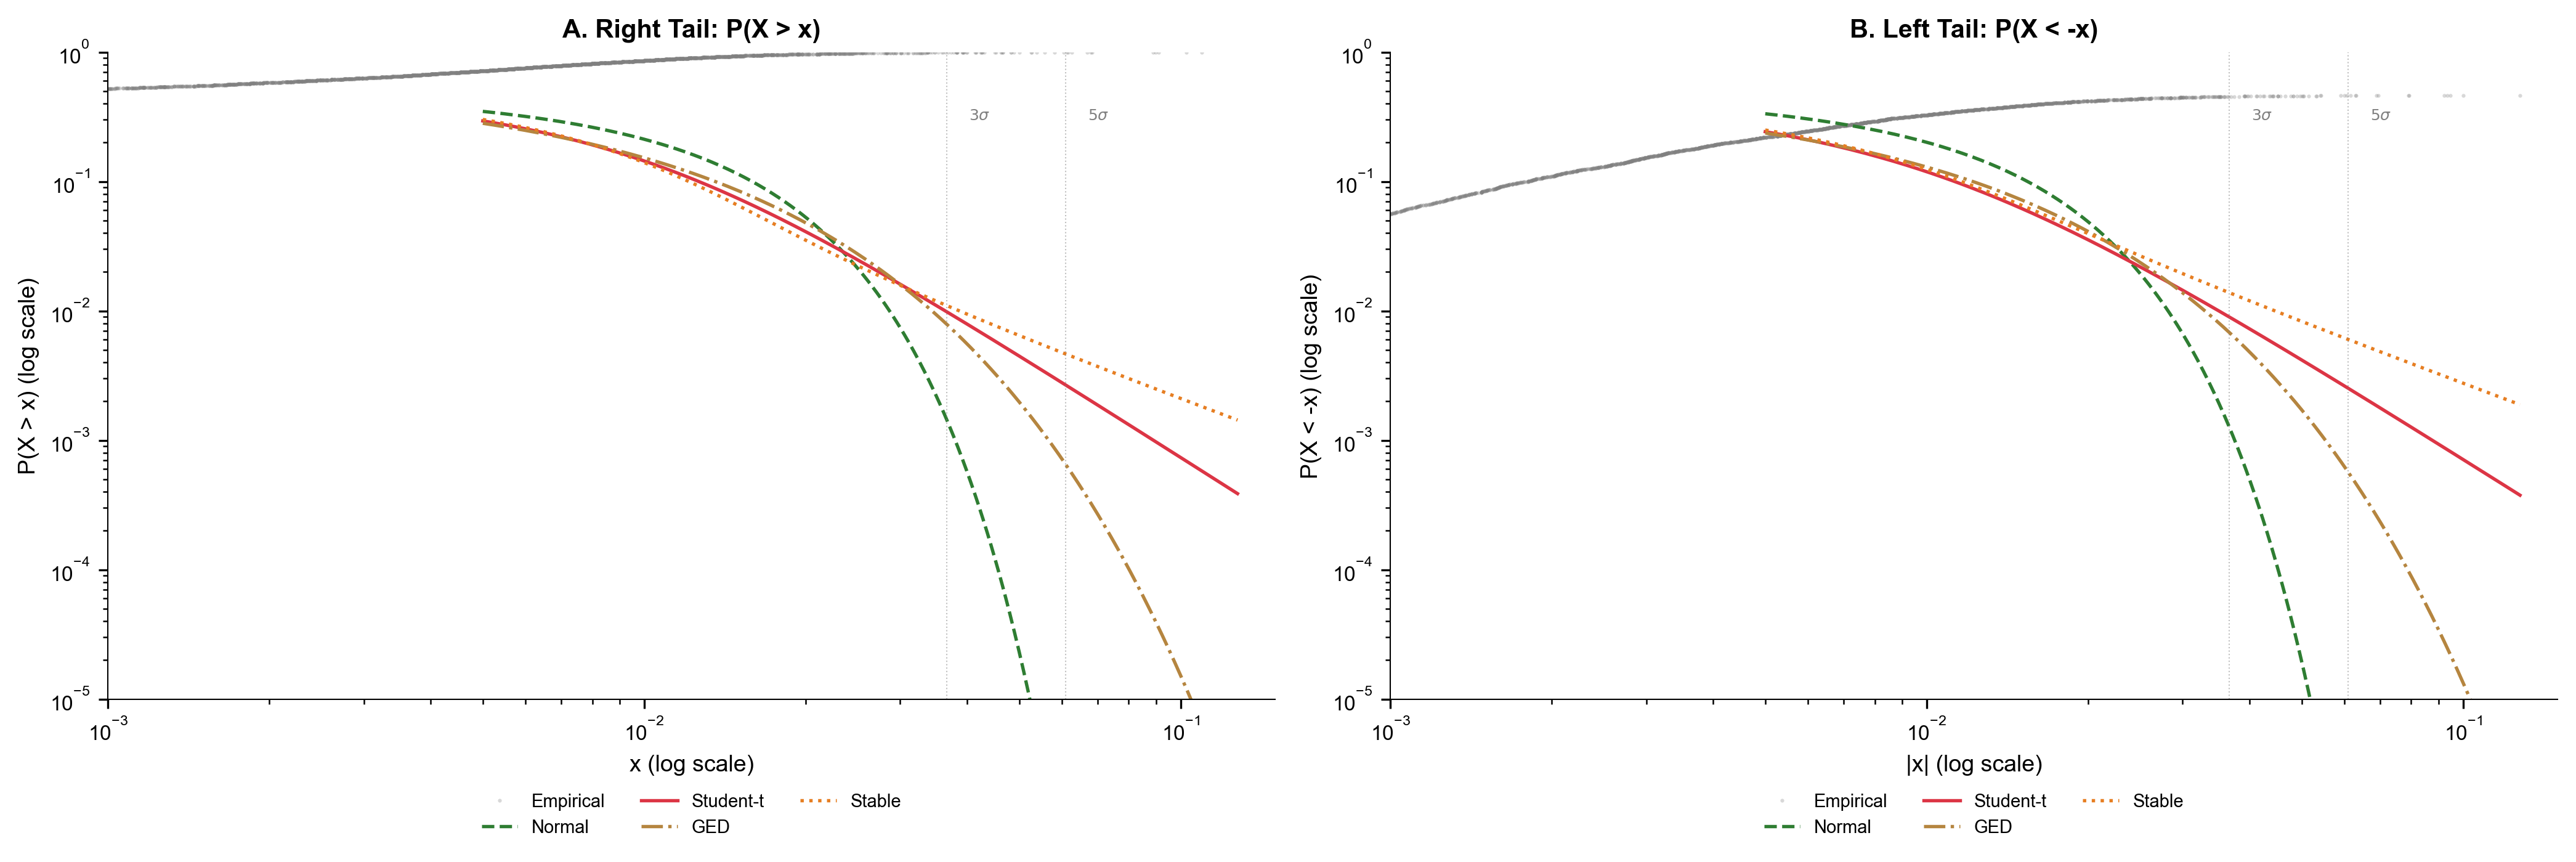
\includegraphics[width=0.65\textwidth]{ch2_dist_comparison_tails.png}
\end{center}

\begin{itemize}
\item Plot $\ln P(|X| > x)$ vs.\ $\ln x$
\item Power-law tail: straight line with slope $-\alpha$
\item Normal: curves downward (exponential decay)
\item Student-$t$ and Stable: approximately linear (power-law decay)
\end{itemize}
\end{frame}

%--- MSc Slide 4 ---
\begin{frame}{Information Criteria and Formal Tests}
\begin{itemize}
\item \textbf{AIC/BIC comparison} across distributions:
\end{itemize}

\begin{center}
\renewcommand{\arraystretch}{1.1}
\begin{tabular}{lccc}
\toprule
\textbf{Distribution} & \textbf{$k$} & \textbf{AIC} & \textbf{BIC} \\
\midrule
Normal & 2 & Highest & Highest \\
Student-$t$ & 3 & Lower & Lower \\
Skewed-$t$ & 4 & Lowest & Lowest \\
Stable & 4 & Comparable to skewed-$t$ & Comparable \\
\bottomrule
\end{tabular}
\end{center}

\begin{itemize}
\item \textbf{Kolmogorov--Smirnov}: $D_n = \sup_x |F_n(x) - F_\theta(x)|$
\item \textbf{Anderson--Darling}: weighted CDF distance, more sensitive to tails
\item \textbf{Likelihood ratio test}: for nested models (Normal vs.\ Student-$t$)
\end{itemize}
\end{frame}

%--- MSc Slide 5 ---
\begin{frame}{Comprehensive Model Comparison}
\begin{center}
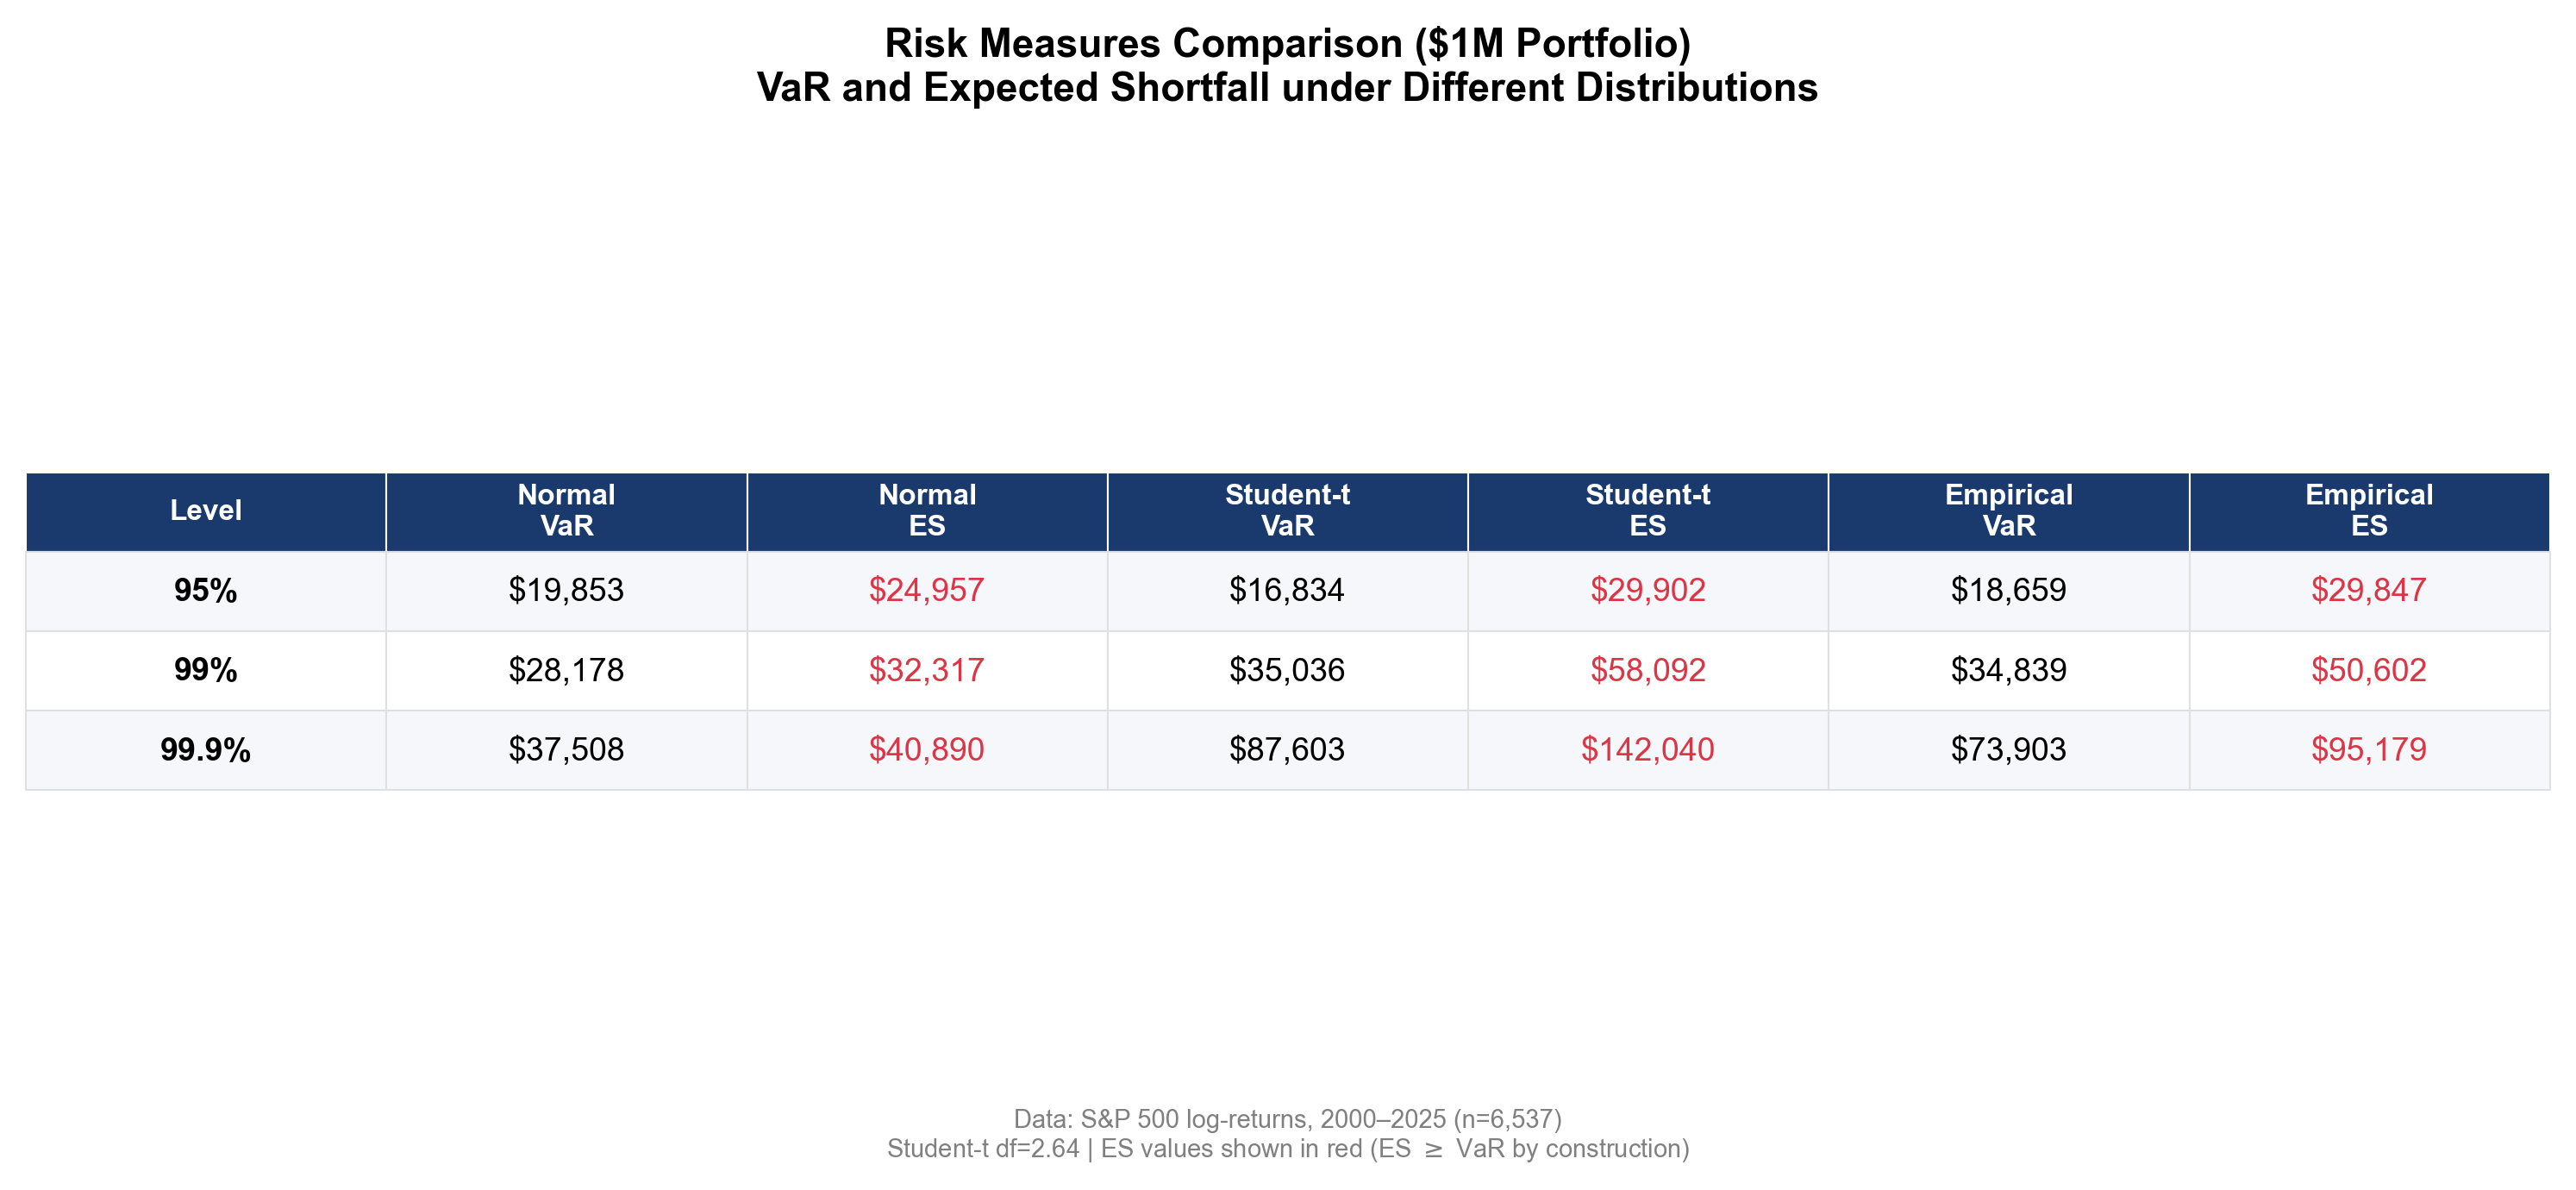
\includegraphics[width=0.65\textwidth]{ch2_risk_comparison_table.png}
\end{center}

\begin{itemize}
\item No single distribution dominates across all criteria
\item Student-$t$ and skewed-$t$: best balance of fit and parsimony
\item Stable: best tail fit but computationally expensive
\item EVT: best for extreme quantiles, but agnostic about center
\end{itemize}
\end{frame}

%--- PhD Slide 6 ---
\begin{frame}{Vuong Test and Scoring Rules}
\begin{itemize}
\item \textbf{Vuong (1989) test}: for comparing non-nested models
\[
V = \frac{\sum_{i=1}^n m_i}{\sqrt{n}\,\hat{\sigma}_m}, \quad m_i = \ln\frac{f_1(x_i;\hat{\theta}_1)}{f_2(x_i;\hat{\theta}_2)}
\]
$V \sim N(0,1)$ under $H_0$: models are equivalent
\item \textbf{CRPS} (Continuous Ranked Probability Score):
\[
\text{CRPS}(F, x) = \int_{-\infty}^{\infty} (F(y) - \mathbf{1}_{y \geq x})^2\,dy
\]
\item Proper scoring rule: encourages honest probabilistic forecasts
\end{itemize}
\end{frame}

%--- PhD Slide 7 ---
\begin{frame}{Predictive Density Evaluation}
\begin{itemize}
\item \textbf{Diebold--Mariano test}: compare predictive densities out-of-sample
\item \textbf{Cross-validation}: $k$-fold evaluation of distributional fit
\item \textbf{Probability Integral Transform (PIT)}:
\begin{itemize}
\item If $F$ is the true CDF, then $U_i = F(X_i) \sim \text{Uniform}(0,1)$
\item Test uniformity of PIT values $\Rightarrow$ test distributional adequacy
\item Rosenblatt (1952) transform for multivariate case
\end{itemize}
\item In-sample fit $\neq$ out-of-sample predictive ability
\item Overfitting risk: complex models (GH, 5 params) may overfit in-sample
\end{itemize}
\end{frame}

%#############################################################################
\section{Risk Management Implications}
%#############################################################################

%--- Y3 Slide 1 ---
\begin{frame}{The Risk Question}
\begin{itemize}
\item A bank holds a portfolio worth \$1{,}000{,}000
\item Fundamental question: \textit{``What is the maximum loss we can expect on a given day, with a specified level of confidence?''}
\item \textbf{Quantile intuition}: the $\alpha$-quantile $q_\alpha$ satisfies:
\[
P(r_t \leq q_\alpha) = \alpha
\]
\item For $\alpha = 0.01$: $q_{0.01}$ is exceeded (downside) only 1\% of the time
\item In 100 trading days, we expect to lose more than $q_{0.01}$ on $\approx 1$ day
\end{itemize}
\end{frame}

%--- Y3 Slide 2 ---
\begin{frame}{Value-at-Risk --- Definition}
\begin{defn}[Value-at-Risk]
The \textbf{Value-at-Risk} at level $\alpha$ is the loss threshold exceeded with probability $\alpha$:
\[
\text{VaR}_\alpha = -q_\alpha = -F^{-1}(\alpha),
\]
where $F$ is the CDF of returns.
\end{defn}

\begin{itemize}
\item With probability $(1-\alpha)$, the daily loss will \textbf{not exceed} $\text{VaR}_\alpha$
\item \textbf{Convention}: ``1\% VaR'' means $\alpha = 0.01$ (loss exceeded with 1\% probability)
\item The minus sign converts the negative quantile into a positive loss amount
\end{itemize}
\end{frame}

%--- Y3 Slide 3 ---
\begin{frame}{VaR under the Normal Assumption}
\begin{itemize}
\item If $r_t \sim N(\mu, \sigma^2)$:
\[
\text{VaR}_\alpha = -(\mu + \sigma \cdot z_\alpha), \quad z_\alpha = \Phi^{-1}(\alpha)
\]
\item \textbf{Example}: $\mu = 0$, $\sigma = 0.015$, portfolio = \$1M, $\alpha = 0.01$:
\[
\text{VaR}_{0.01} = -0.015 \times (-2.326) \times 1{,}000{,}000 = \$34{,}890
\]
\item On 99 out of 100 trading days, loss will not exceed \$34{,}890
\end{itemize}

\begin{center}
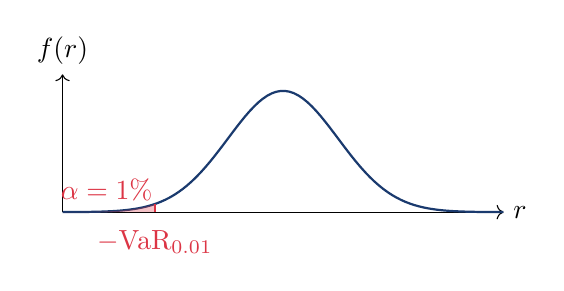
\begin{tikzpicture}[scale=0.7]
\draw[->] (-4,0) -- (4,0) node[right] {$r$};
\draw[->] (-4,0) -- (-4,2.5) node[above] {$f(r)$};
\draw[MainBlue, thick, domain=-4:4, samples=100] plot (\x, {2.2*exp(-\x*\x/2)});
\fill[Crimson, opacity=0.3, domain=-4:-2.326, samples=50] plot (\x, {2.2*exp(-\x*\x/2)}) -- (-2.326,0) -- (-4,0) -- cycle;
\draw[Crimson, thick, dashed] (-2.326,0) -- (-2.326,{2.2*exp(-2.326*2.326/2)});
\node[below, Crimson] at (-2.326,-0.15) {$-\text{VaR}_{0.01}$};
\node[Crimson] at (-3.2,0.4) {$\alpha = 1\%$};
\end{tikzpicture}
\end{center}
\end{frame}

%--- Y3 Slide 4 ---
\begin{frame}{Why the Distribution Matters for VaR}
\begin{center}
\renewcommand{\arraystretch}{1.0}
\scriptsize
\begin{tabular}{l c c c}
\toprule
\textbf{Model} & \textbf{1\% VaR (\$1M)} & \textbf{0.1\% VaR (\$1M)} & \textbf{Ratio to Normal} \\
\midrule
Normal & \$27{,}000 & \$35{,}900 & 1.0$\times$ \\
Student-$t$ ($\nu=5$) & \$33{,}700 & \$58{,}400 & 1.6$\times$ \\
Stable ($\alpha=1.7$) & \$41{,}000 & \$90{,}200 & 2.5$\times$ \\
\bottomrule
\end{tabular}
\end{center}
\begin{itemize}
\item At 1\% level: moderate difference ($\sim$25\%); at 0.1\%: \textbf{dramatic} (1.6--2.5$\times$)
\item \textbf{Conclusion}: Distribution choice directly affects required capital
\end{itemize}
\begin{center}
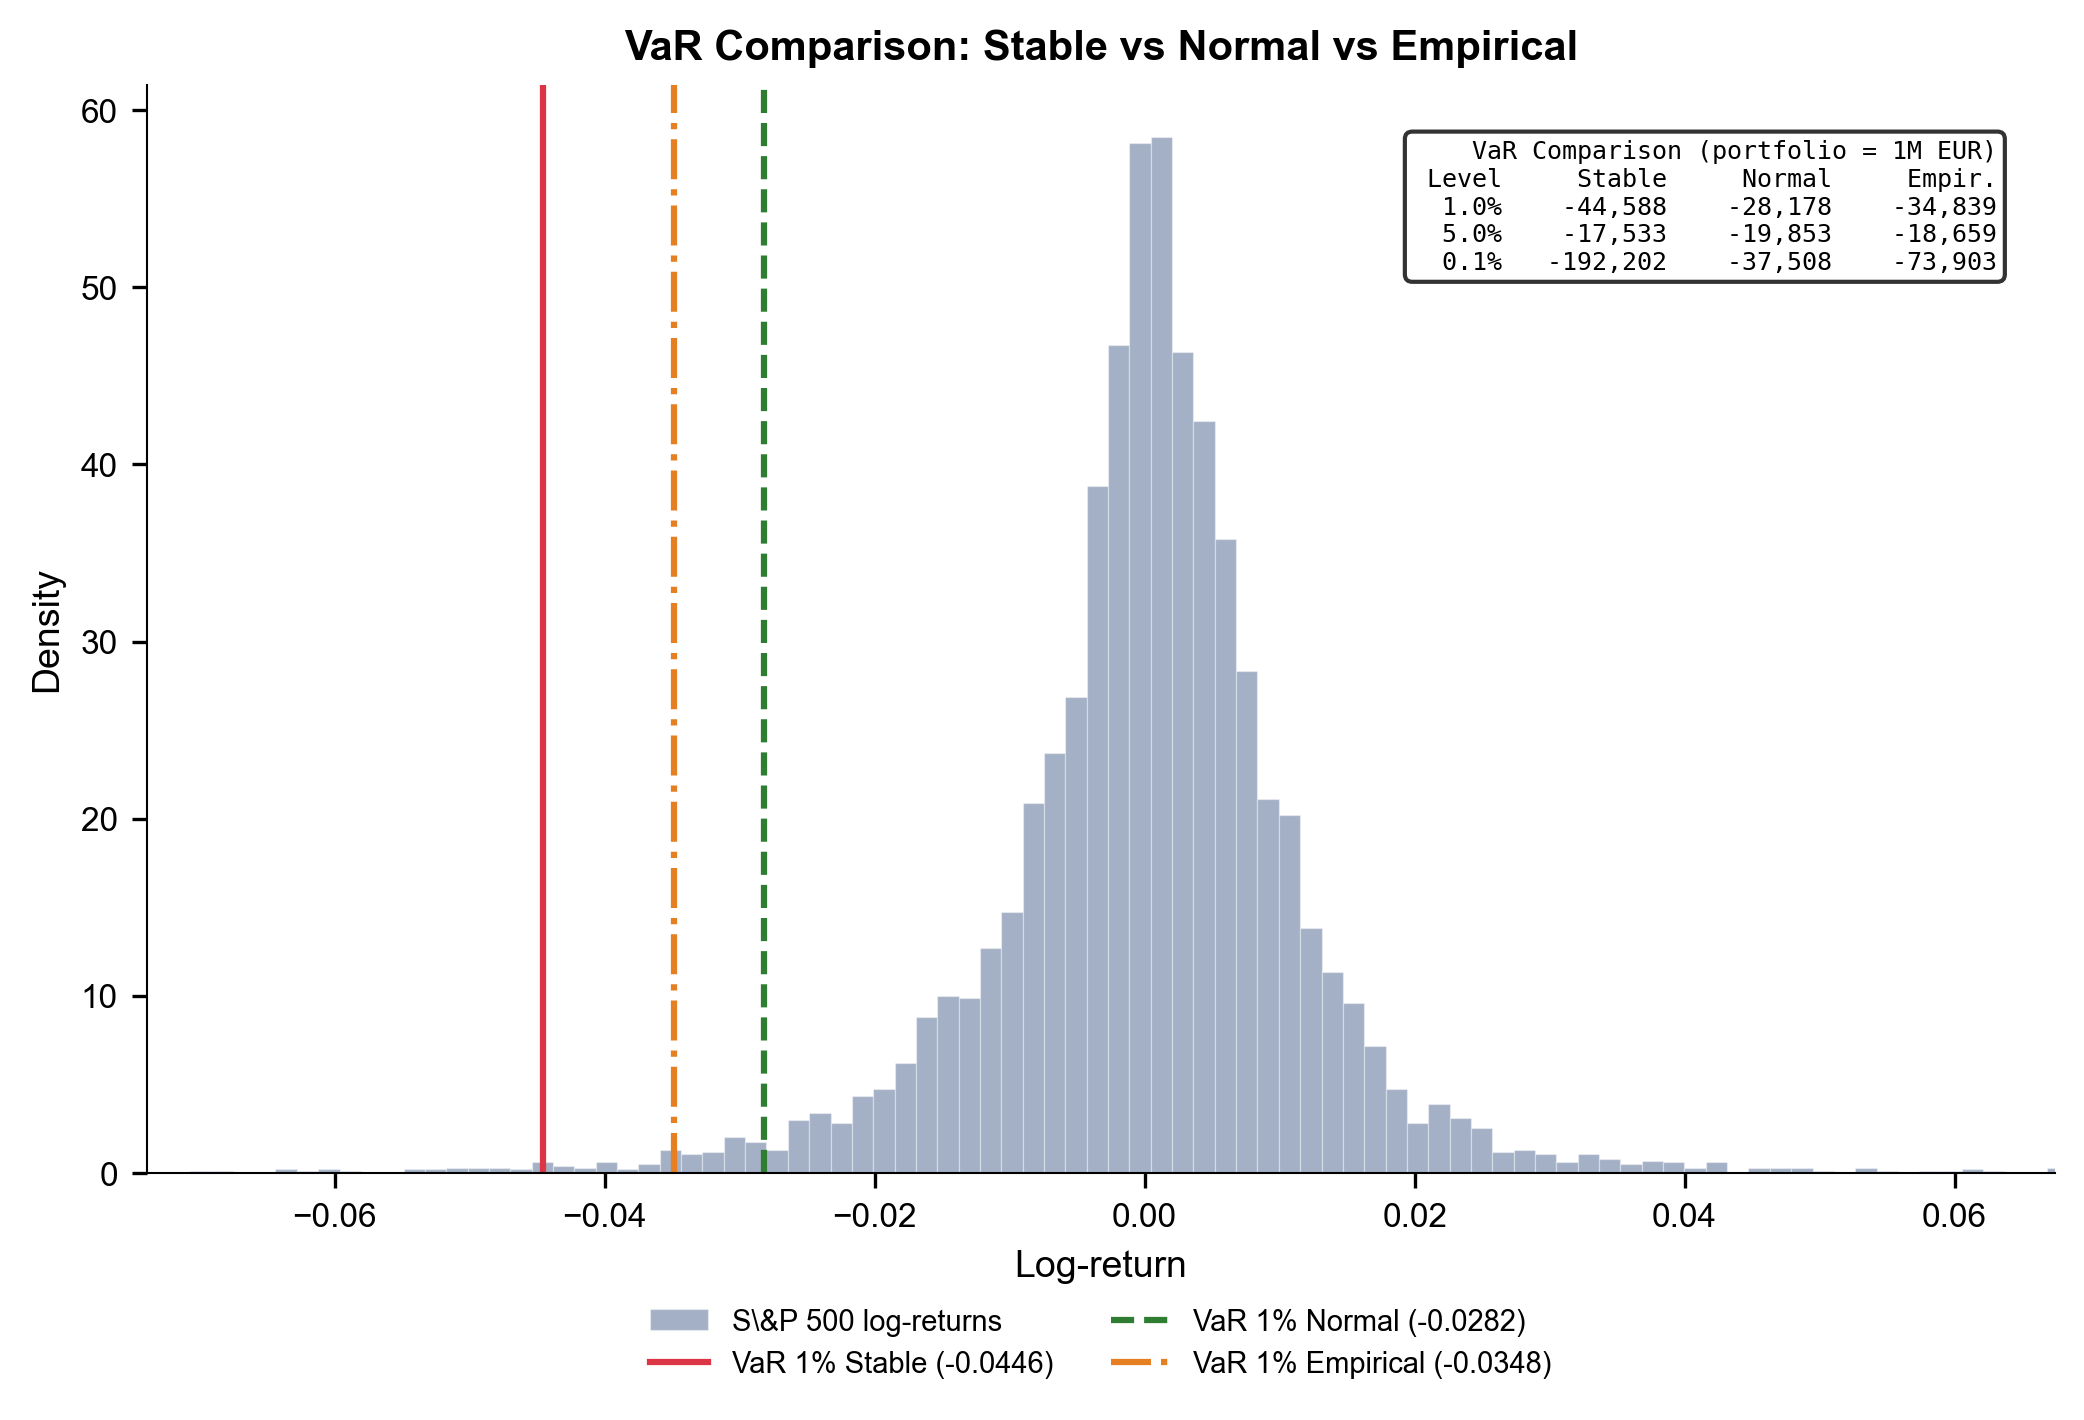
\includegraphics[width=0.4\textwidth]{ch2_var_comparison.png}
\end{center}
\end{frame}

%--- Y3 Slide 5 ---
\begin{frame}{Limitations of VaR}
\begin{itemize}
\item VaR tells us the \textit{threshold} of the worst $\alpha$-fraction of days
\item But \textbf{not} how bad things get \textit{beyond} that threshold
\item VaR does not distinguish between ``losing \$35k'' and ``losing \$200k'' --- both are ``VaR exceedances''
\item A better measure (\textbf{Expected Shortfall}) addresses this limitation
\end{itemize}

\vspace{0.3cm}
\begin{alertblock}{VaR is Not Subadditive}
\begin{itemize}
\item Diversification can \textit{increase} VaR: $\text{VaR}(X+Y) > \text{VaR}(X) + \text{VaR}(Y)$ is possible
\item This contradicts the principle that diversification reduces risk
\end{itemize}
\end{alertblock}
\end{frame}

%--- MSc Slide 6 ---
\begin{frame}{Expected Shortfall}
\begin{defn}[Expected Shortfall]
The \textbf{Expected Shortfall} (Conditional VaR) at level $\alpha$:
\[
\text{ES}_\alpha = -\frac{1}{\alpha}\int_0^\alpha F^{-1}(p)\,dp = \E[-X \mid X \leq -\text{VaR}_\alpha].
\]
\end{defn}

\begin{itemize}
\item \textbf{Interpretation}: average loss given we are in the worst $\alpha\%$ of days
\item Under normality: $\text{ES}_\alpha = -\mu + \sigma\frac{\phi(\Phi^{-1}(\alpha))}{\alpha}$
\item ES is a \textbf{coherent} risk measure (subadditive):
\[
\text{ES}(X+Y) \leq \text{ES}(X) + \text{ES}(Y)
\]
\item Diversification always reduces ES (unlike VaR)
\end{itemize}
\end{frame}

%--- MSc Slide 7 ---
\begin{frame}{Backtesting and Basel Framework}
\begin{itemize}
\item \textbf{Kupiec test}: $LR_{uc} = -2\ln\frac{\alpha^x(1-\alpha)^{n-x}}{\hat{\alpha}^x(1-\hat{\alpha})^{n-x}} \sim \chi^2(1)$
\begin{itemize}
\item $x$ = number of VaR exceedances in $n$ days; $H_0$: true rate $= \alpha$
\end{itemize}
\item \textbf{Christoffersen test}: independence of exceedances (no clustering)
\item \textbf{Basel III/IV}: shift from 1\% VaR (10-day) to 2.5\% ES
\item Traffic light: Green (0--4), Yellow (5--9), Red (10+) per 250 days
\end{itemize}
\vspace{-0.2cm}
\begin{center}
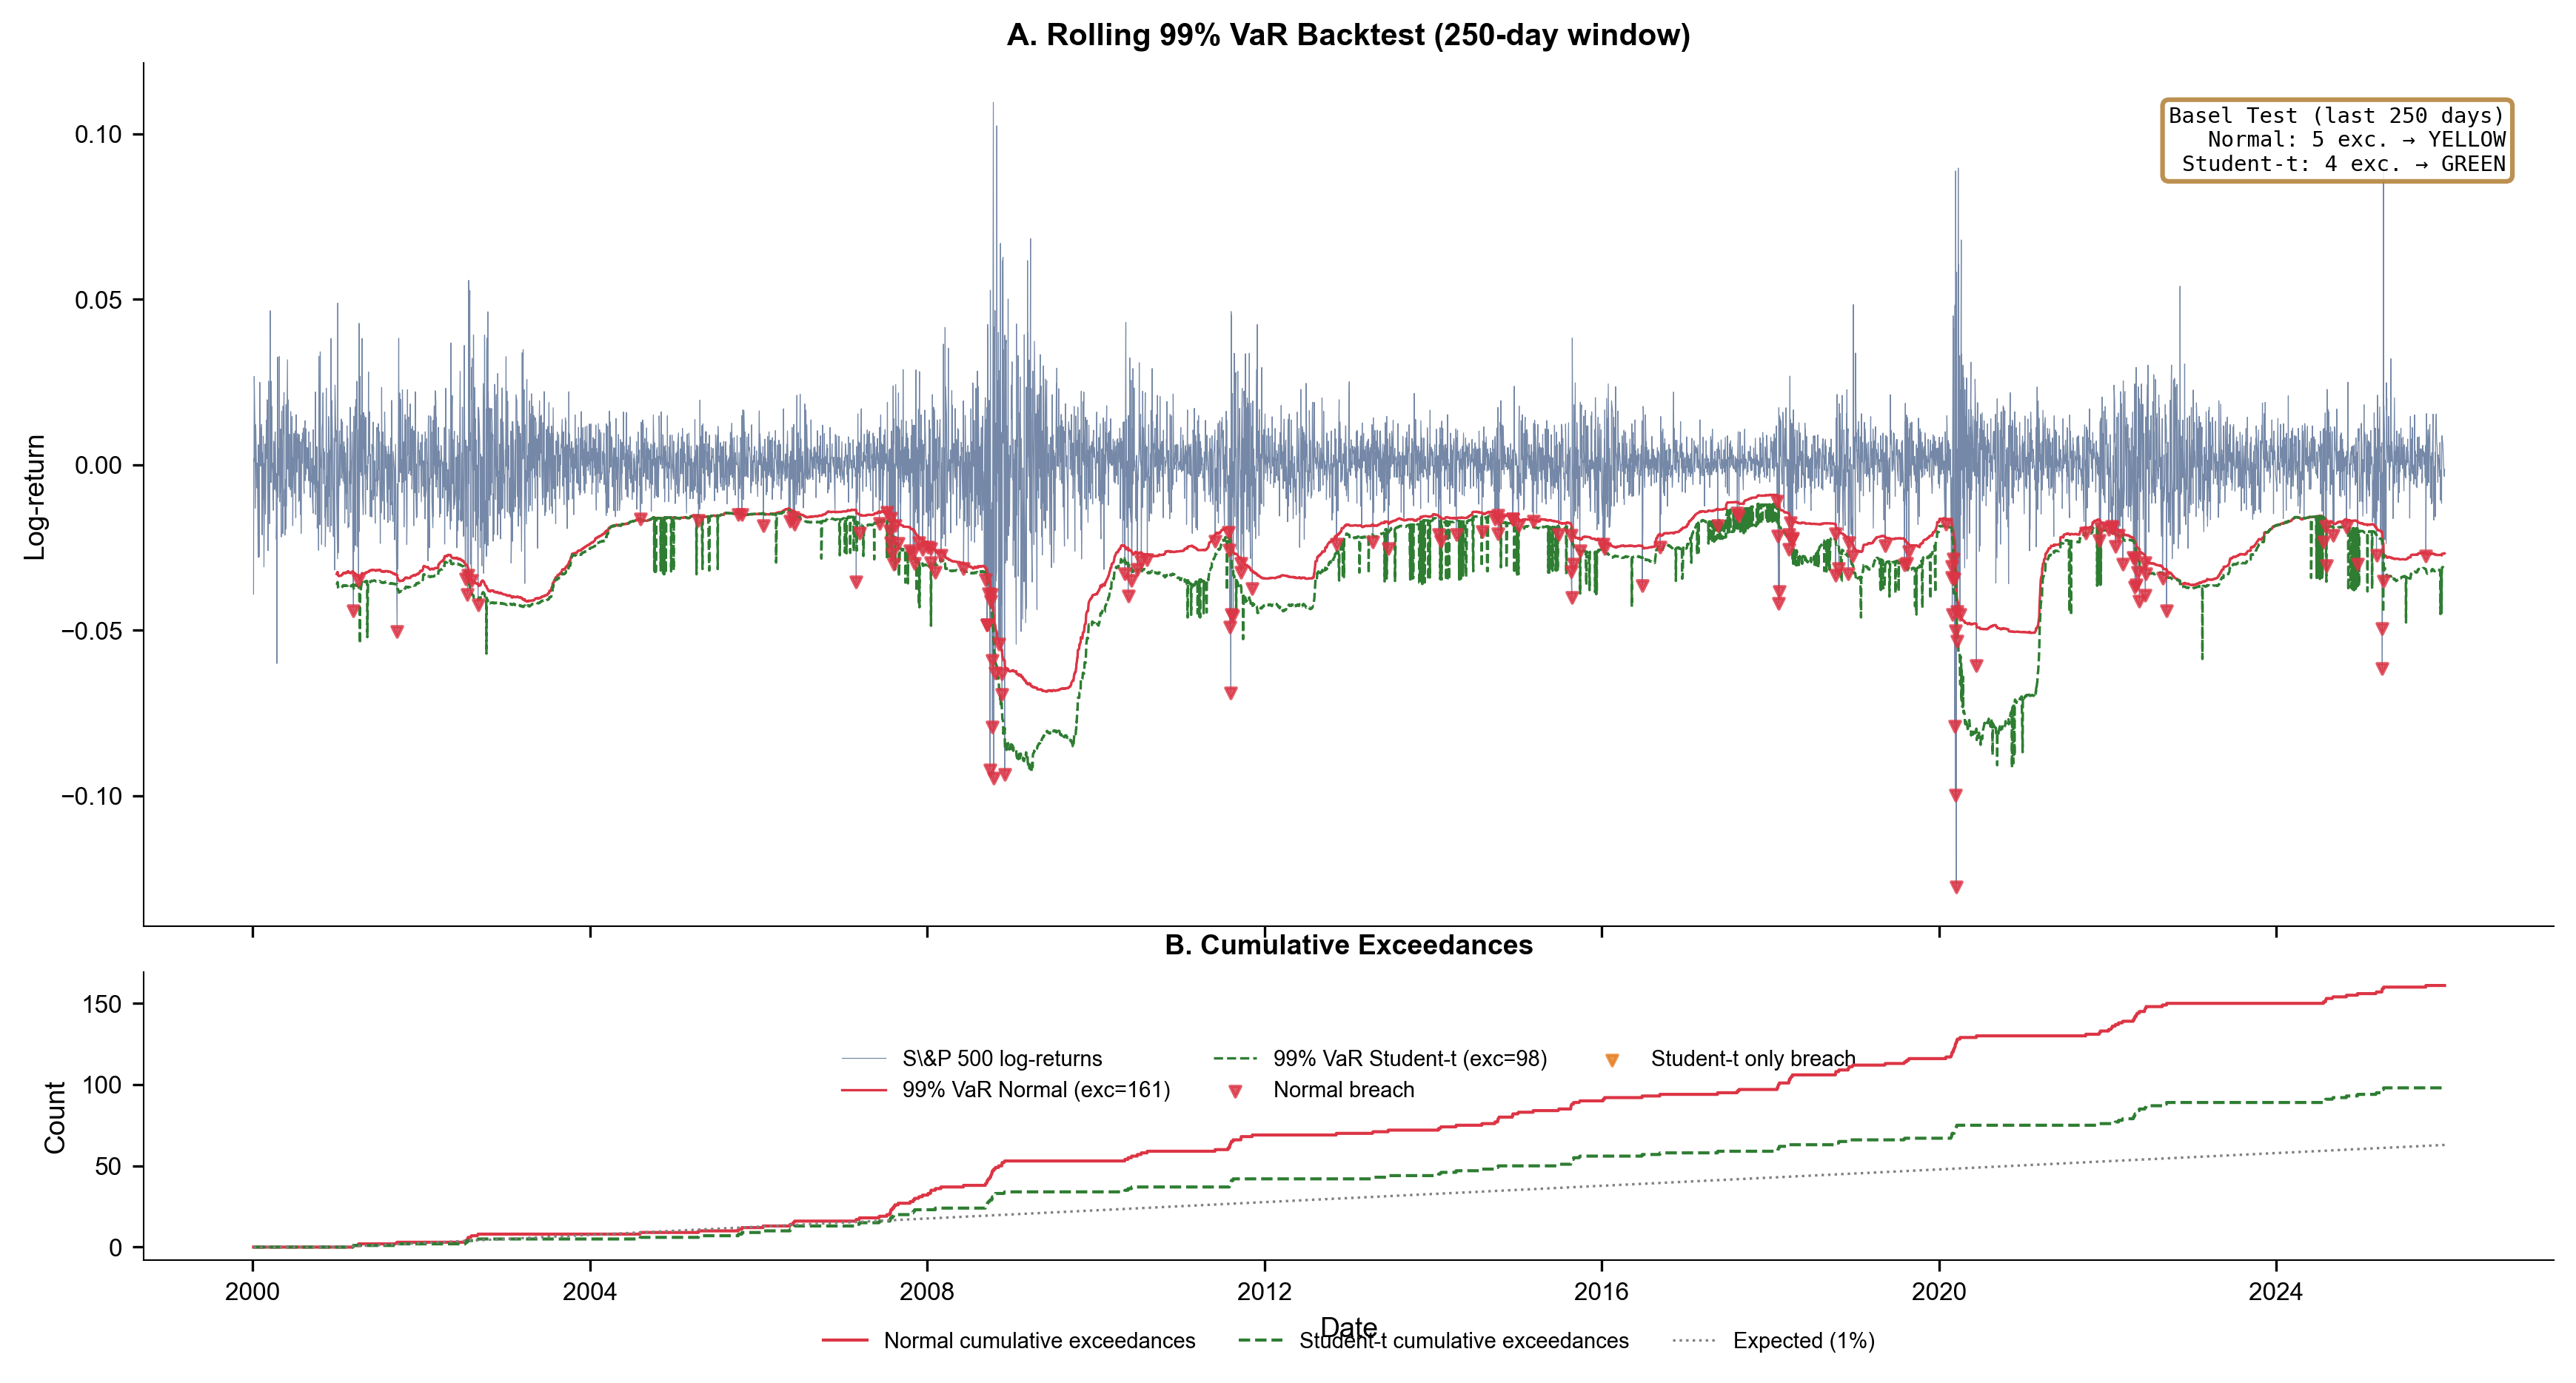
\includegraphics[width=0.45\textwidth]{ch2_var_backtest.png}
\end{center}
\end{frame}

%--- MSc Slide 8 ---
\begin{frame}{VaR Backtest Results}
\begin{center}
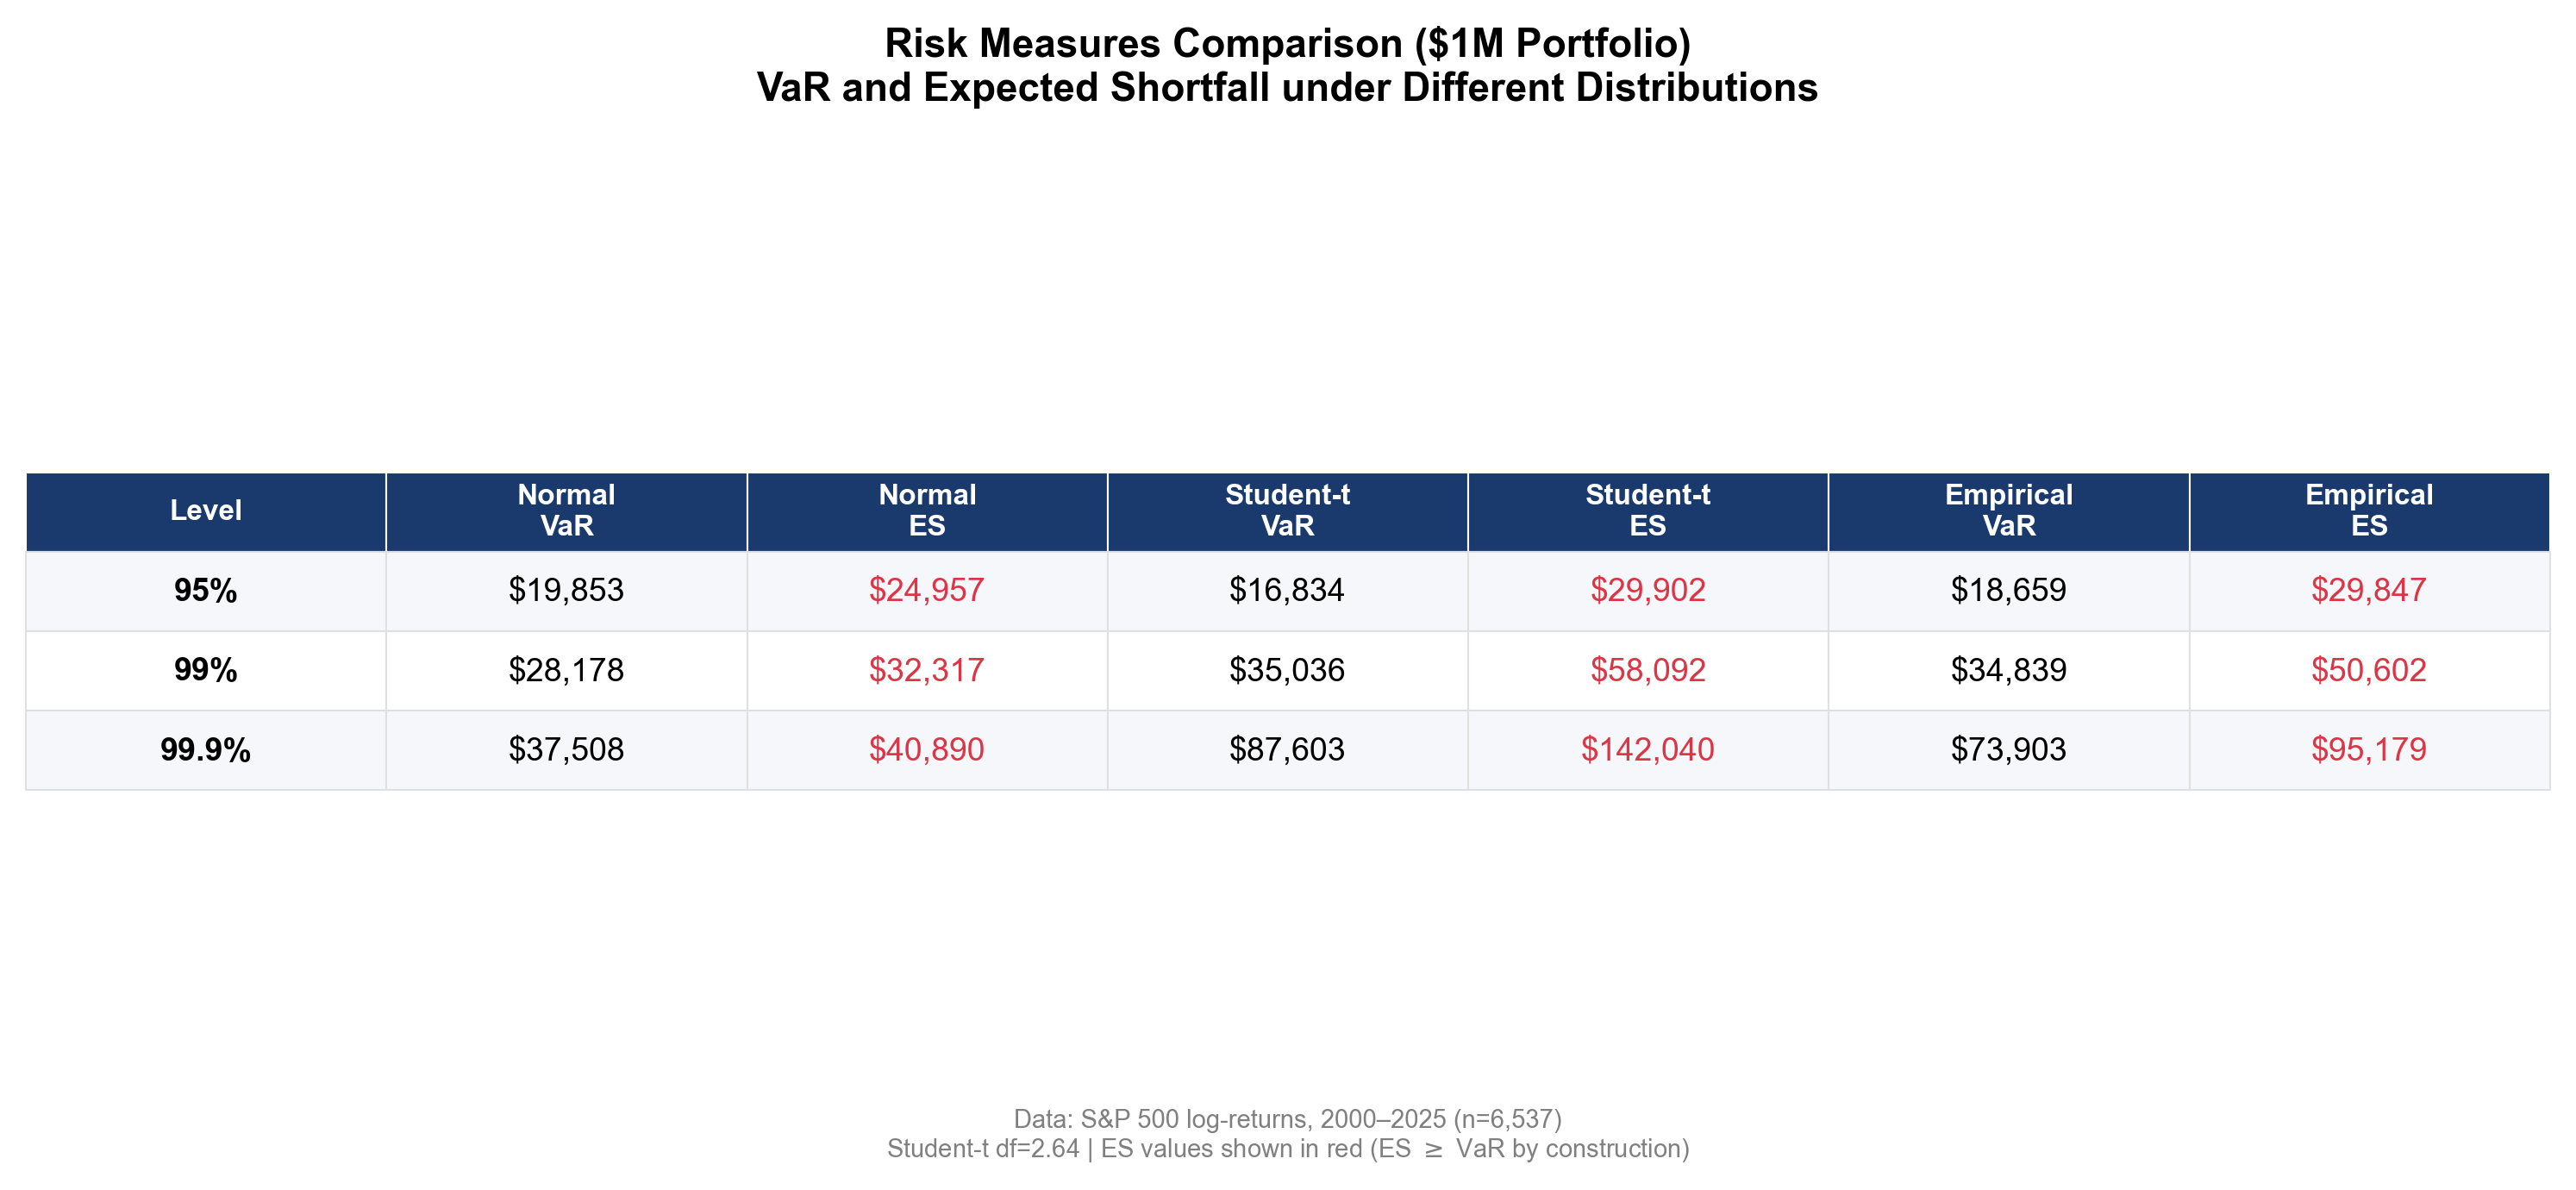
\includegraphics[width=0.65\textwidth]{ch2_risk_comparison_table.png}
\end{center}

\begin{itemize}
\item Normal: too many VaR exceedances $\Rightarrow$ rejected by Kupiec test
\item Student-$t$: exceedances close to expected rate
\item EVT-based: conservative but robust
\item \textbf{Model risk}: capital reserves depend on the model chosen
\end{itemize}
\end{frame}

%--- PhD Slide 9 ---
\begin{frame}{Spectral Risk Measures and Elicitability}
\begin{itemize}
\item \textbf{Spectral risk measures}:
\[
\rho_\phi(X) = -\int_0^1 \phi(p)\,F^{-1}(p)\,dp
\]
with risk spectrum $\phi(p) \geq 0$, $\int_0^1 \phi(p)\,dp = 1$, $\phi$ non-decreasing
\item VaR: $\phi(p) = \delta(p - \alpha)$; \quad ES: $\phi(p) = \frac{1}{\alpha}\mathbf{1}_{p \leq \alpha}$
\item \textbf{Elicitability} (Gneiting, 2011):
\begin{itemize}
\item VaR is elicitable: optimal under quantile loss $\rho(x,q) = (\alpha - \mathbf{1}_{x<q})(x-q)$
\item ES is \textbf{not} elicitable alone
\item (VaR, ES) is jointly elicitable (Fissler \& Ziegel, 2016)
\end{itemize}
\end{itemize}
\end{frame}

%--- PhD Slide 10 ---
\begin{frame}{Capital Allocation and Model Risk}
\begin{itemize}
\item \textbf{Euler allocation}: allocate portfolio ES to individual positions:
\[
\text{ES}_i = \E[-X_i \mid X_{\text{total}} \leq -\text{VaR}_\alpha]
\]
\item Distributional assumptions directly affect allocated capital per desk
\item \textbf{Stable distributions and extreme risk}: ES under stable diverges as $\alpha \to 0$ faster than under Student-$t$
\item \textbf{Model risk quantification}: compute VaR/ES under multiple models; the range quantifies model uncertainty
\item Regulatory response: stressed VaR, model risk add-ons
\end{itemize}
\end{frame}

%#############################################################################
\section{Modern Extensions}
%#############################################################################

%--- Y3 Slide 1 ---
\begin{frame}{GARCH --- Intuition}
\begin{itemize}
\item Returns are uncorrelated but \textbf{not independent}: volatility changes over time
\item \textbf{GARCH(1,1)}: variance depends on past shocks and past variance:
\[
\sigma_t^2 = \omega + \alpha\epsilon_{t-1}^2 + \beta\sigma_{t-1}^2
\]
\item $\alpha$: reaction to shocks; $\beta$: persistence; $\alpha + \beta < 1$: stationarity
\item After GARCH filtering, standardized residuals $z_t = \epsilon_t/\sigma_t$ are approximately i.i.d.
\item But $z_t$ still shows \textbf{excess kurtosis} $\Rightarrow$ use Student-$t$ or skewed-$t$ innovations
\end{itemize}
\end{frame}

%--- MSc Slide 2 ---
\begin{frame}{GARCH with Non-Gaussian Innovations}
\begin{itemize}
\item \textbf{GARCH-$t$}: $r_t = \mu + \sigma_t z_t$, \quad $z_t \sim t_\nu$
\item Captures both volatility clustering and heavy tails
\item \textbf{Asymmetric GARCH}:
\begin{itemize}
\item GJR-GARCH: $\sigma_t^2 = \omega + (\alpha + \gamma\,\mathbf{1}_{\epsilon_{t-1}<0})\epsilon_{t-1}^2 + \beta\sigma_{t-1}^2$
\item EGARCH: $\ln\sigma_t^2 = \omega + \alpha|z_{t-1}| + \gamma z_{t-1} + \beta\ln\sigma_{t-1}^2$
\end{itemize}
\item $\gamma > 0$ in GJR or $\gamma < 0$ in EGARCH captures the \textbf{leverage effect}
\end{itemize}

\vspace{-0.1cm}
\begin{center}
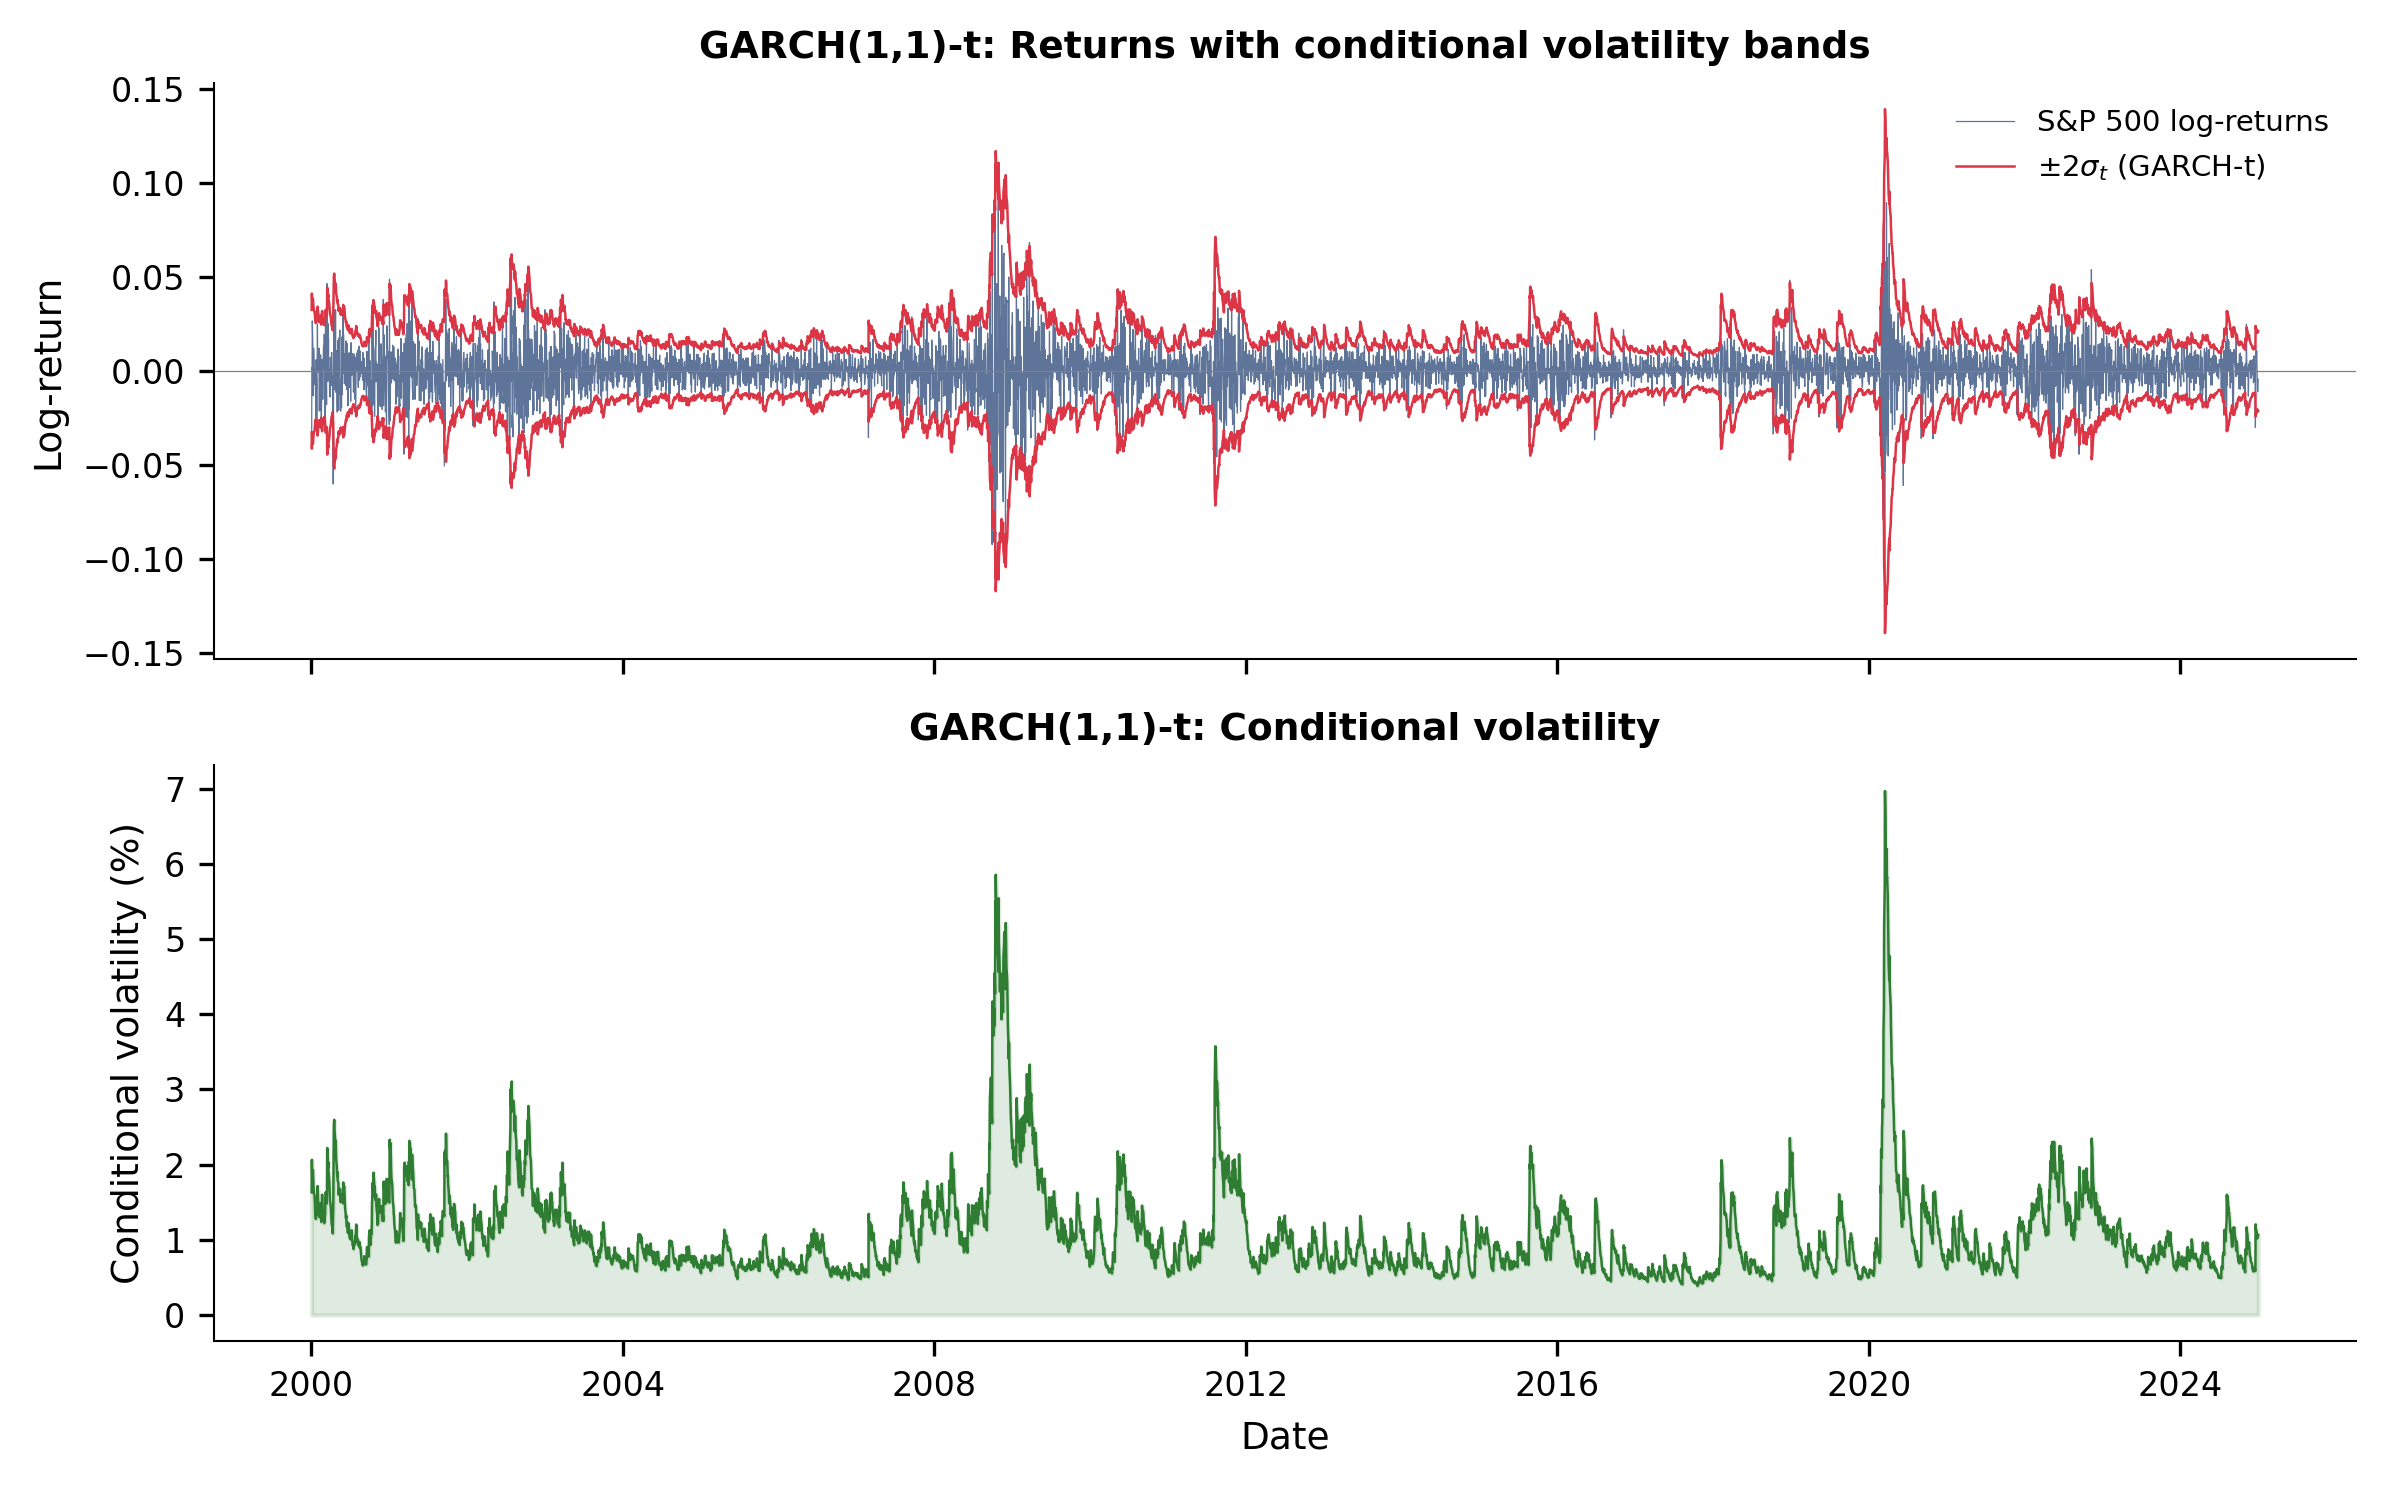
\includegraphics[width=0.40\textwidth]{ch2_garch_t_fit.png}
\end{center}
\end{frame}

%--- MSc Slide 3 ---
\begin{frame}{Gaussian Mixtures and Regime Switching}
\begin{columns}[T]
\begin{column}{0.55\textwidth}
\textbf{Gaussian mixtures}:
\[
f(x) = \sum_{k=1}^K \pi_k\,\phi(x;\mu_k, \sigma_k^2)
\]
\begin{itemize}
\item $K=2$: calm regime ($\sigma_1$ small) + crisis regime ($\sigma_2$ large)
\item EM algorithm for estimation
\end{itemize}

\vspace{0.2cm}
\textbf{Hamilton (1989) regime switching}:
\begin{itemize}
\item Latent Markov chain $s_t \in \{1,2\}$
\item $r_t \mid s_t \sim N(\mu_{s_t}, \sigma_{s_t}^2)$
\item Transition probabilities estimated via MLE
\end{itemize}
\end{column}
\begin{column}{0.43\textwidth}
\begin{center}
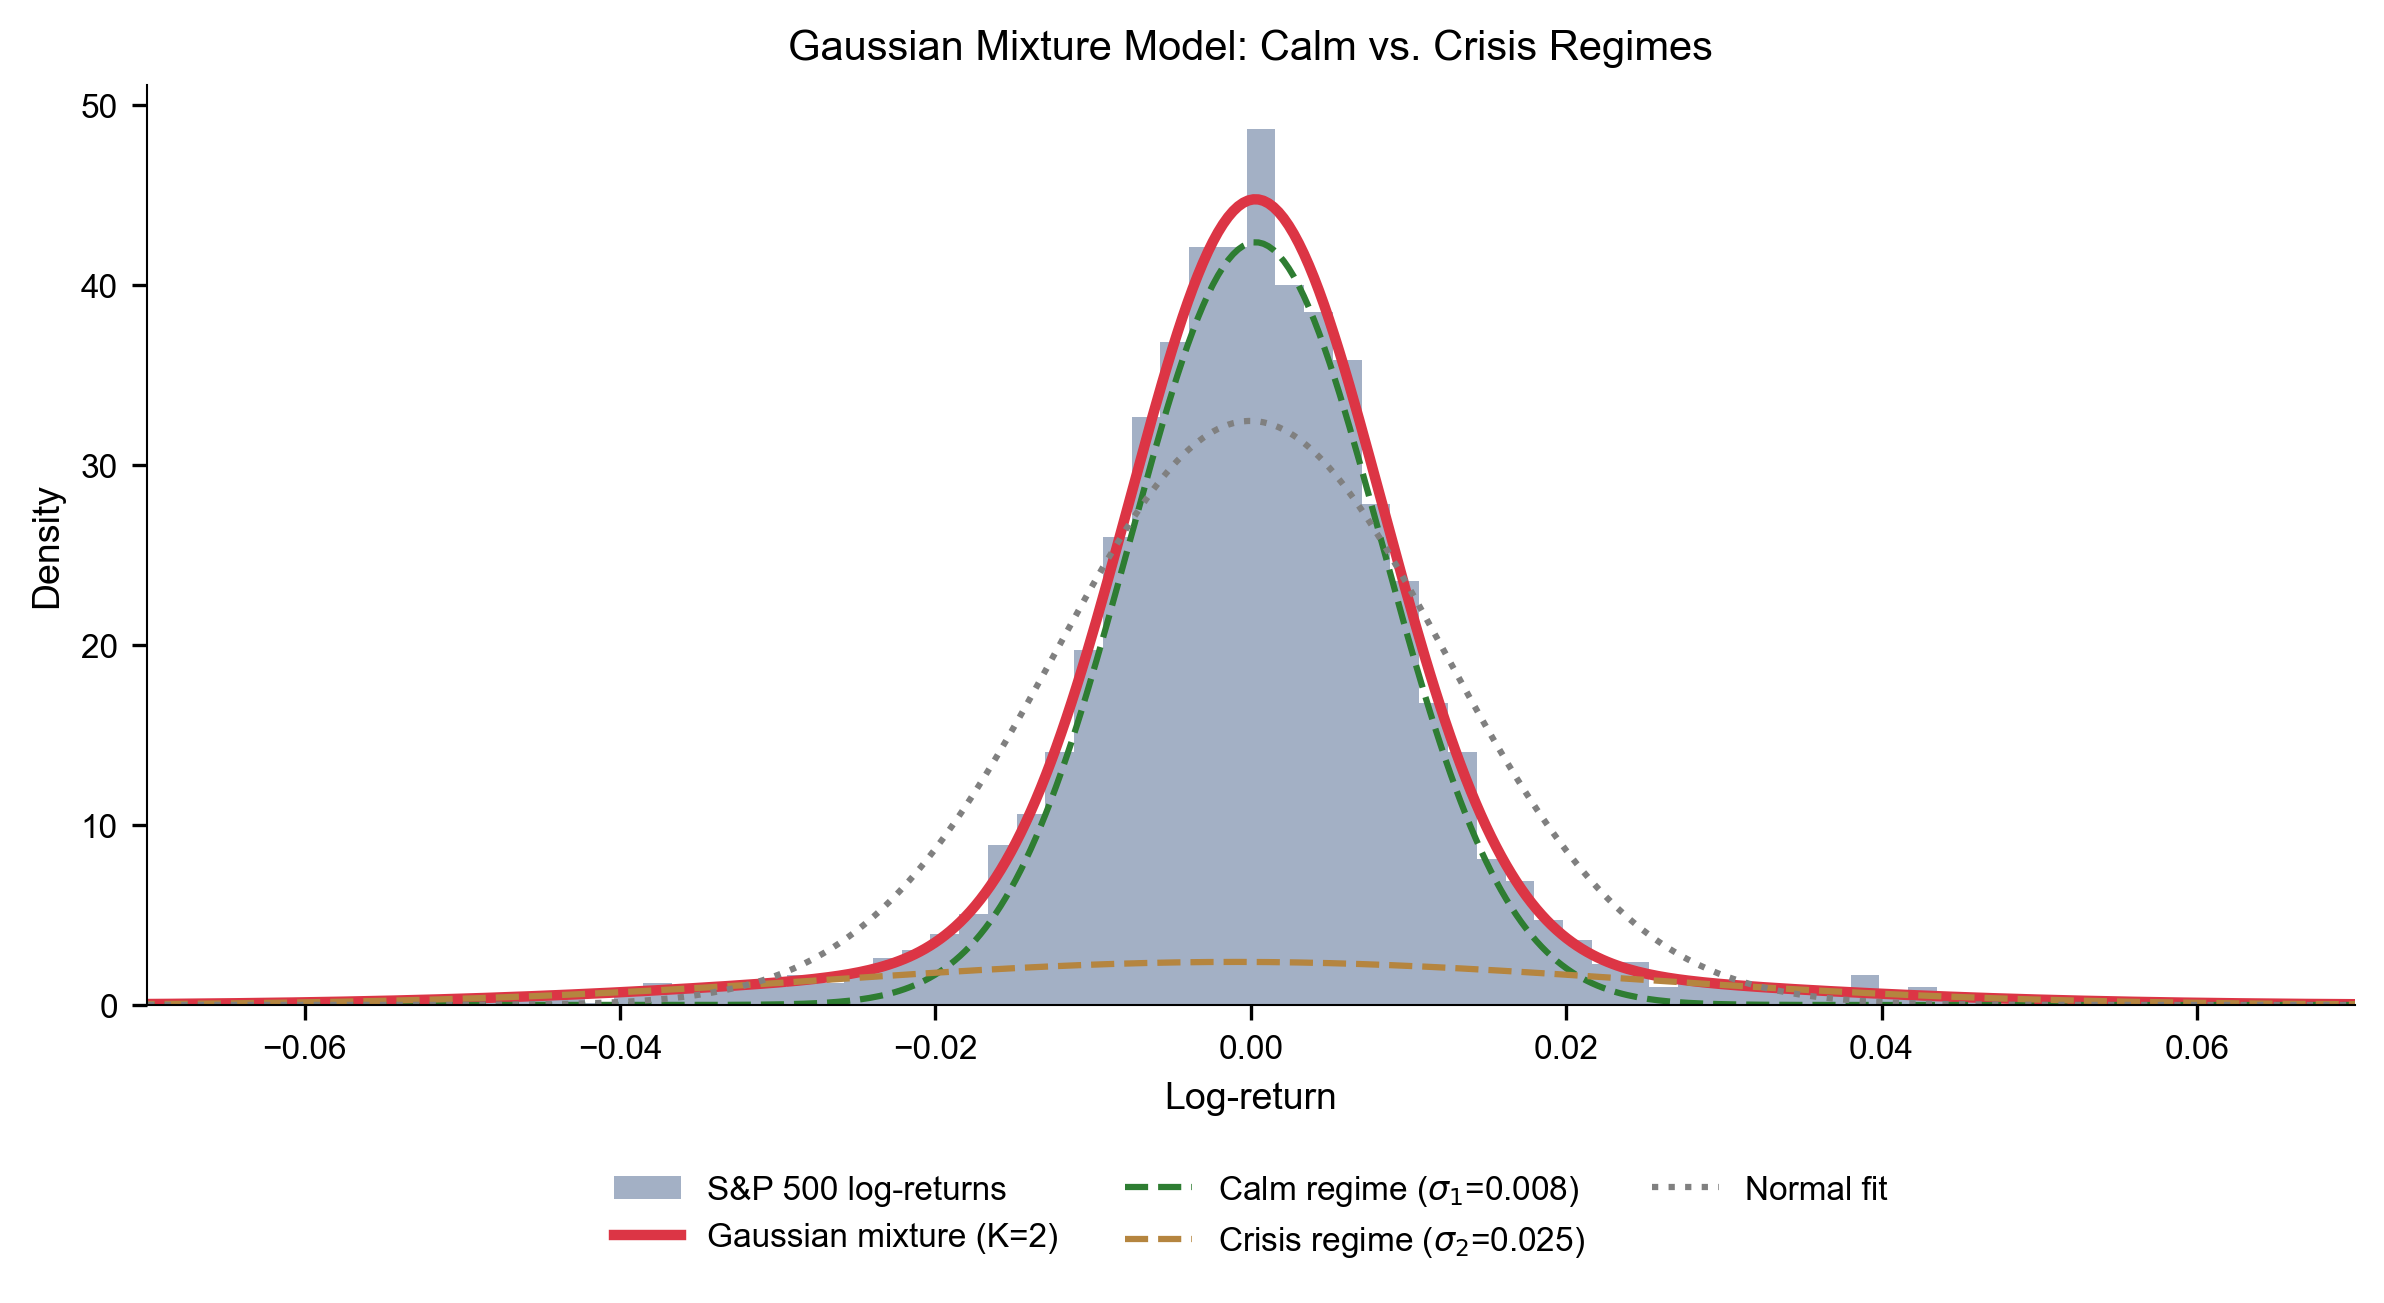
\includegraphics[width=\textwidth]{ch2_gaussian_mixture.png}
\end{center}
\end{column}
\end{columns}
\end{frame}

%--- MSc Slide 4 ---
\begin{frame}{Regime Classification}
\begin{center}
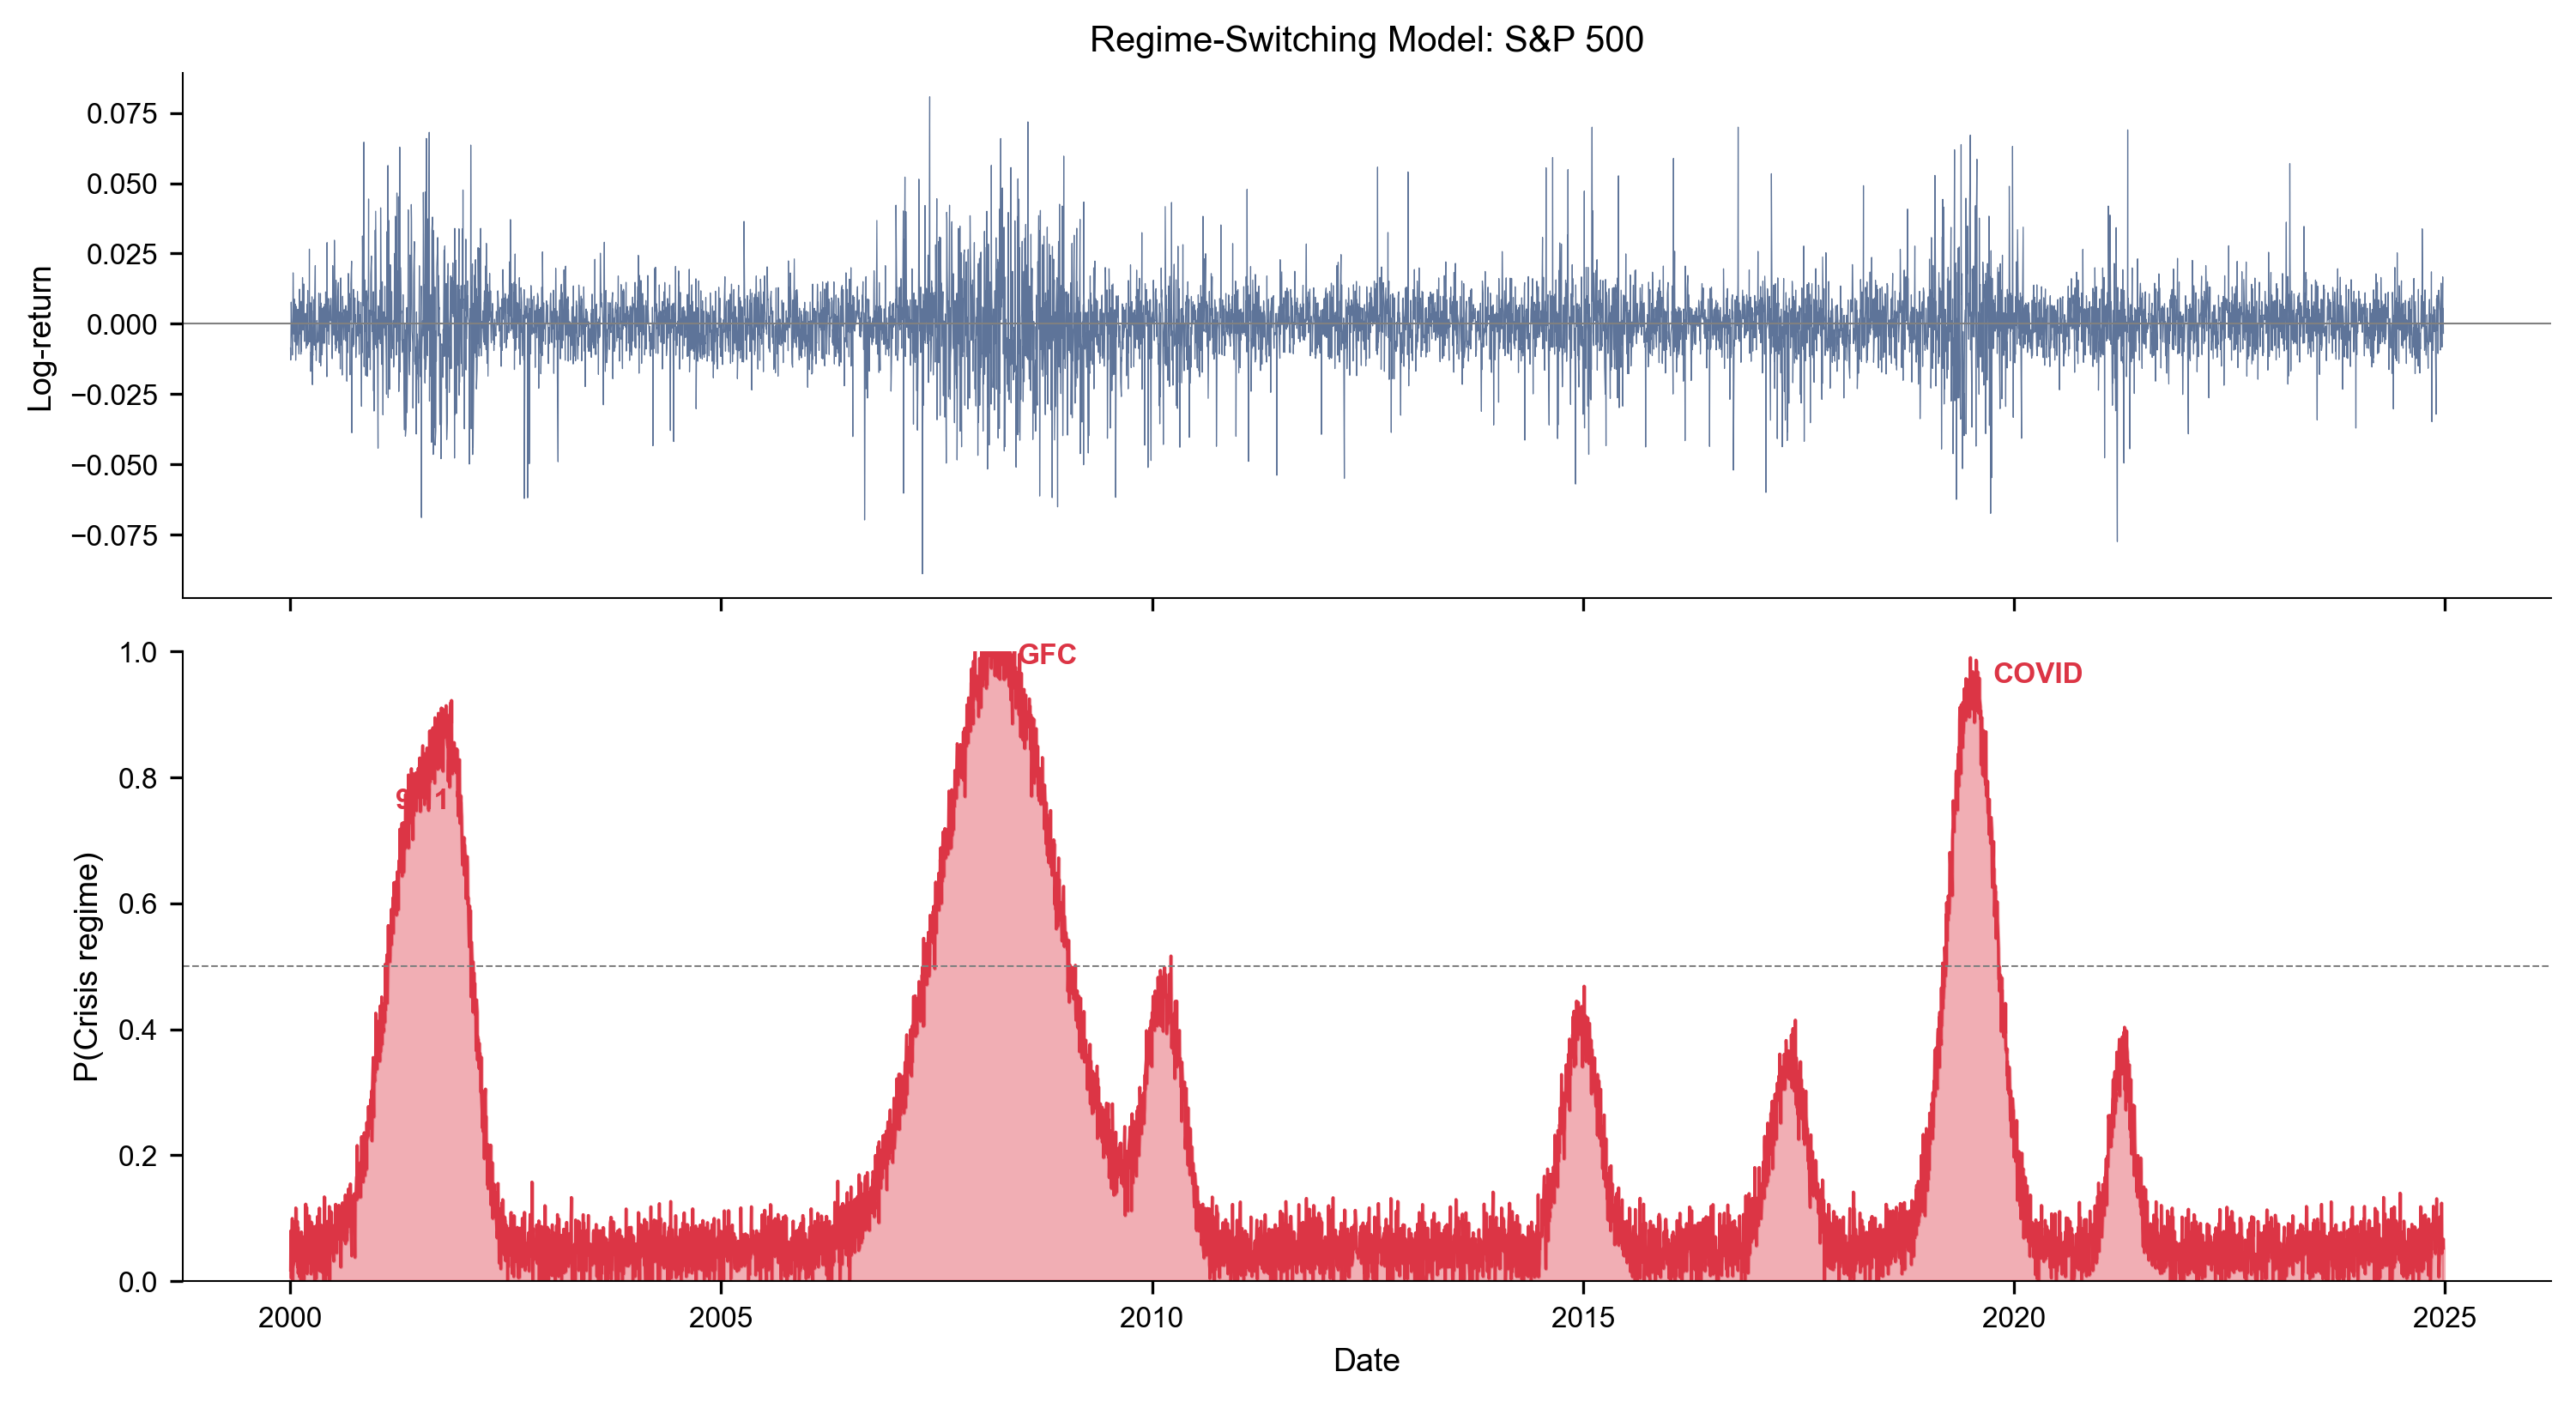
\includegraphics[width=0.58\textwidth]{ch2_regime_classification.png}
\end{center}
\vspace{-0.2cm}
\begin{itemize}
\item Smooth probability of being in ``crisis'' regime
\item Crisis periods: 2001, 2008--2009, 2020
\item Regime-switching captures time-varying tail risk
\end{itemize}
\end{frame}

%--- PhD Slide 5 ---
\begin{frame}{Stochastic Volatility and Jump-Diffusion}
\begin{itemize}
\item \textbf{Stochastic volatility}:
\[
d\ln\sigma_t^2 = \kappa(\theta - \ln\sigma_t^2)\,dt + \sigma_v\,dW_t^v
\]
with $\Corr(dW_t, dW_t^v) = \rho$ (leverage)
\item \textbf{Jump-diffusion} (Merton, 1976):
\[
dS/S = \mu\,dt + \sigma\,dW + J\,dN_t
\]
where $N_t$ is a Poisson process, $J \sim N(\mu_J, \sigma_J^2)$
\item Kou (2002): double-exponential jumps for analytical tractability
\item These models generate heavy tails and volatility clustering simultaneously
\end{itemize}
\end{frame}

%--- PhD Slide 6 ---
\begin{frame}{L\'{e}vy-Driven Models}
\begin{itemize}
\item \textbf{BNS model} (Barndorff-Nielsen \& Shephard, 2001):
\[
dX_t = (\mu + \beta\sigma_t^2)\,dt + \sigma_t\,dW_t, \quad d\sigma_t^2 = -\lambda\sigma_t^2\,dt + dL_{\lambda t}
\]
where $L_t$ is a subordinator (increasing L\'{e}vy process)
\item \textbf{GARCH with stable innovations}: Mittnik \& Rachev (1993)
\item \textbf{Realized volatility}: $RV_t = \sum_{i=1}^{M} r_{t,i}^2$ (high-frequency)
\item Fractionally integrated GARCH (FIGARCH) for long memory in volatility
\end{itemize}
\end{frame}

%--- PhD Slide 7 ---
\begin{frame}{Realized Measures and Microstructure}
\begin{itemize}
\item \textbf{Realized variance}: $RV_t = \sum_{i=1}^M r_{t,i}^2 \xrightarrow{p} \int_0^1 \sigma_s^2\,ds$ as $M \to \infty$
\item \textbf{Microstructure noise}: at very high frequencies, bid-ask bounce biases $RV$ upward
\item \textbf{Corrections}: subsampling, kernel estimators (Barndorff-Nielsen et al., 2008)
\item \textbf{Jump detection}: bipower variation separates continuous and jump components
\item Distribution of returns \textit{conditional on} realized volatility is closer to Gaussian (time-deformation)
\end{itemize}
\end{frame}

%#############################################################################
\section{Case Study}
%#############################################################################

%--- Y3 Slide 1: Data ---
\begin{frame}{Case Study: The Data}
\quantlet{SFM\_ch2\_case\_study\_2a}{https://github.com/QuantLet/Stat_fin_markets/tree/master/Ch_02/SFM_ch2_case_study_2a}
\begin{block}{Prices and log-returns}
\begin{itemize}\setlength\itemsep{2pt}
\item \textcolor{MainBlue}{\textbf{S\&P 500}} --- developed market, high liquidity
\item \textcolor{IDAred}{\textbf{BRD}} --- Romanian stock, emerging market
\item \textcolor{Forest}{\textbf{Bitcoin}} --- digital asset, extreme volatility
\item Period: 2015--2025, daily data
\end{itemize}
\end{block}
\vspace{0.1cm}
\begin{center}
{\small
\begin{tabular}{lrrrrr}
\toprule
\textbf{Asset} & \textbf{N} & \textbf{Mean (\%)} & \textbf{Std (\%)} & \textbf{Skew} & \textbf{Kurt} \\
\midrule
S\&P 500 & $\sim$2\,500 & 0.05 & 1.15 & $-$0.60 & 13.5 \\
BRD      & $\sim$2\,500 & 0.04 & 1.10 & $-$0.80 & 12.0 \\
Bitcoin   & $\sim$3\,600 & 0.12 & 3.80 & $-$0.30 & 8.5 \\
\bottomrule
\end{tabular}}
\end{center}
\end{frame}

%--- Y3 Slide 1b: Chart full ---
\begin{frame}{Case Study: Prices and Log-Returns}
\begin{center}
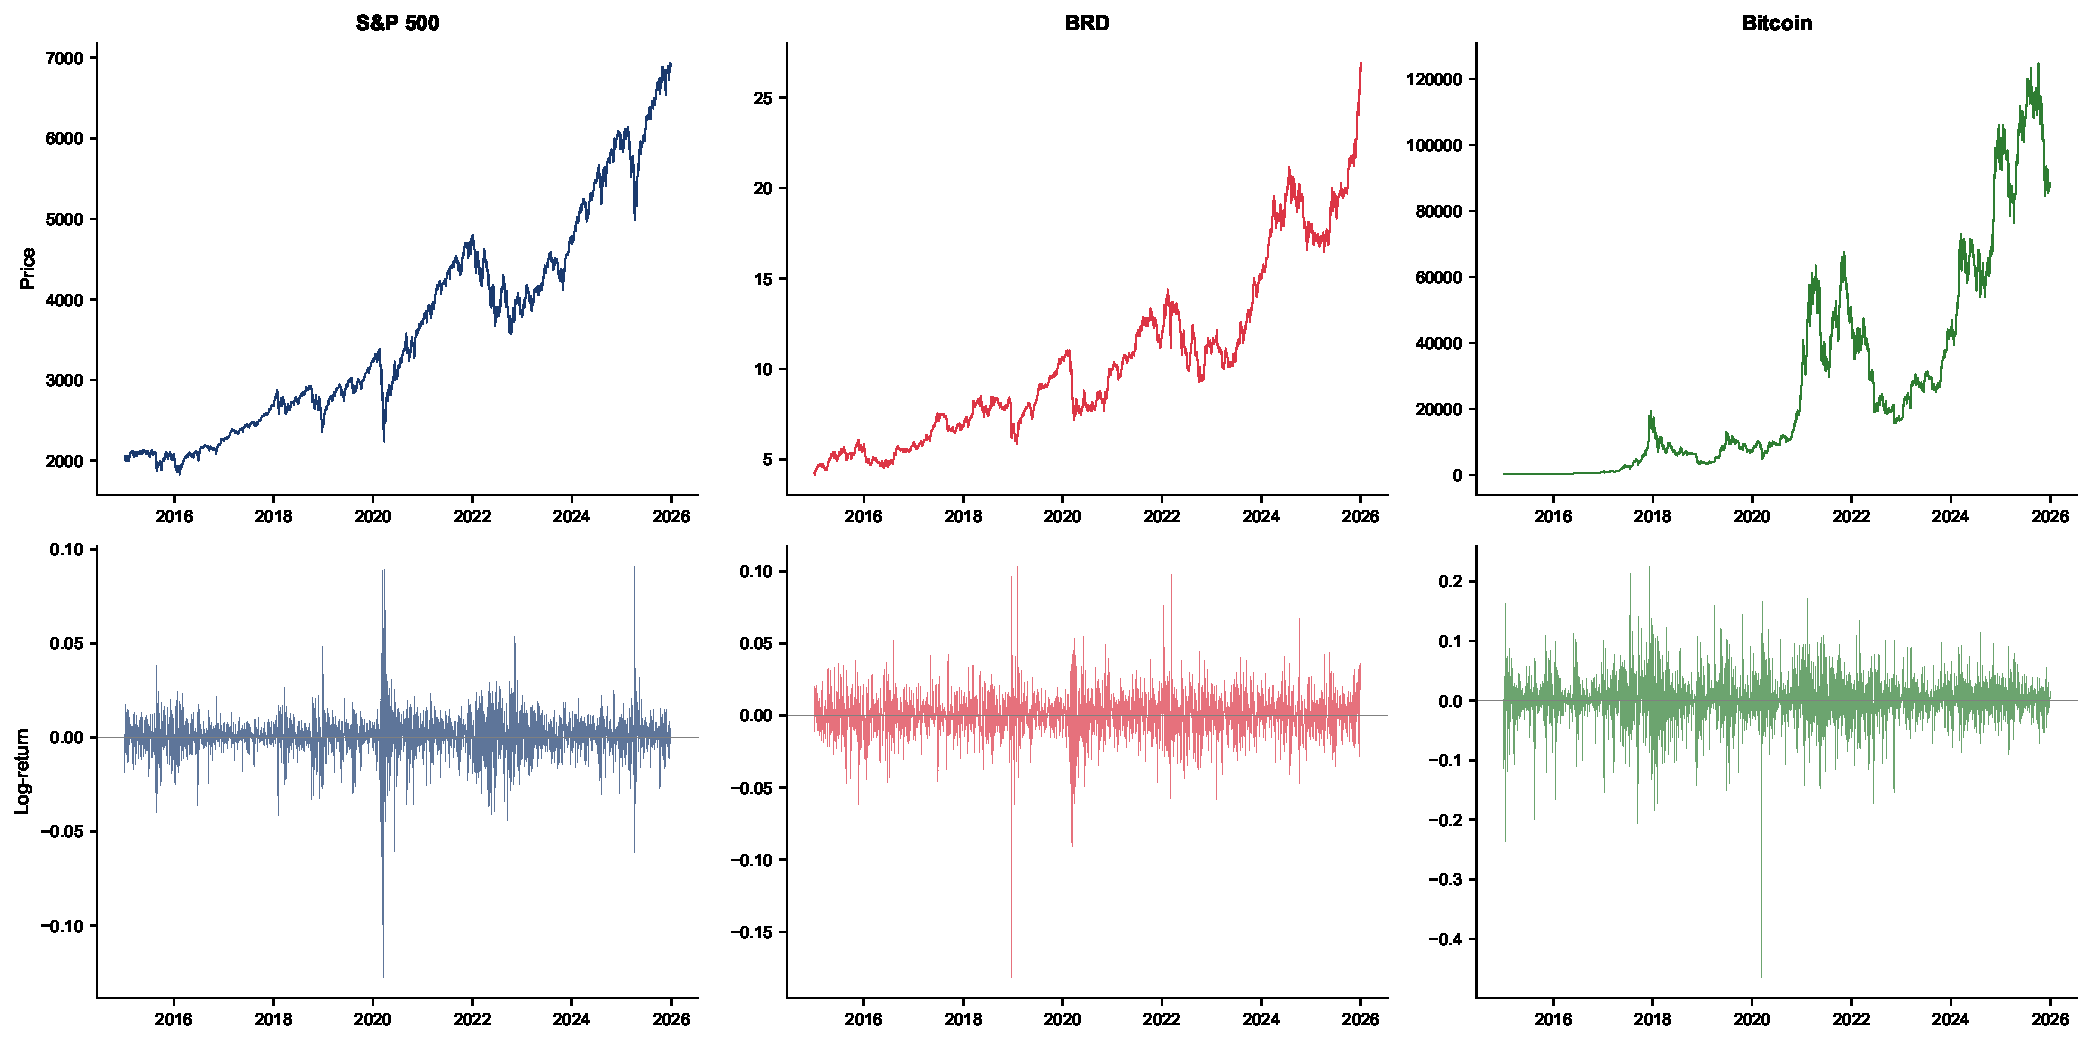
\includegraphics[width=0.82\textwidth]{../../charts/ch2_cs2a_price_returns.pdf}
\end{center}
\vspace{-0.3cm}
\quantlet{SFM\_ch2\_case\_study\_2a}{https://github.com/QuantLet/Stat_fin_markets/tree/master/Ch_02/SFM_ch2_case_study_2a}
\end{frame}

%--- Y3 Slide 2: Stylized facts ---
\begin{frame}{Case Study: Stylized Facts}
\quantlet{SFM\_ch2\_case\_study\_2a}{https://github.com/QuantLet/Stat_fin_markets/tree/master/Ch_02/SFM_ch2_case_study_2a}
\begin{block}{Volatility clustering}
\begin{itemize}\setlength\itemsep{2pt}
\item ACF of $|r_t|$ confirms long-range dependence
\item All 3 assets exhibit significant autocorrelation of $|r_t|$ up to lag 60
\item \textbf{Kurtosis} $\gg 3$ across all markets $\Rightarrow$ heavy tails
\item \textbf{Negative skewness} for S\&P 500 and BRD (\emph{leverage effect})
\item Bitcoin: lower skewness, but 3$\times$ higher volatility
\end{itemize}
\end{block}
\begin{rmk}
\begin{itemize}
\item Volatility clustering invalidates the i.i.d.\ assumption required by the Black--Scholes model
\end{itemize}
\end{rmk}
\end{frame}

%--- Y3 Slide 2b: Chart full ---
\begin{frame}{Case Study: Stylized Facts --- Chart}
\begin{center}
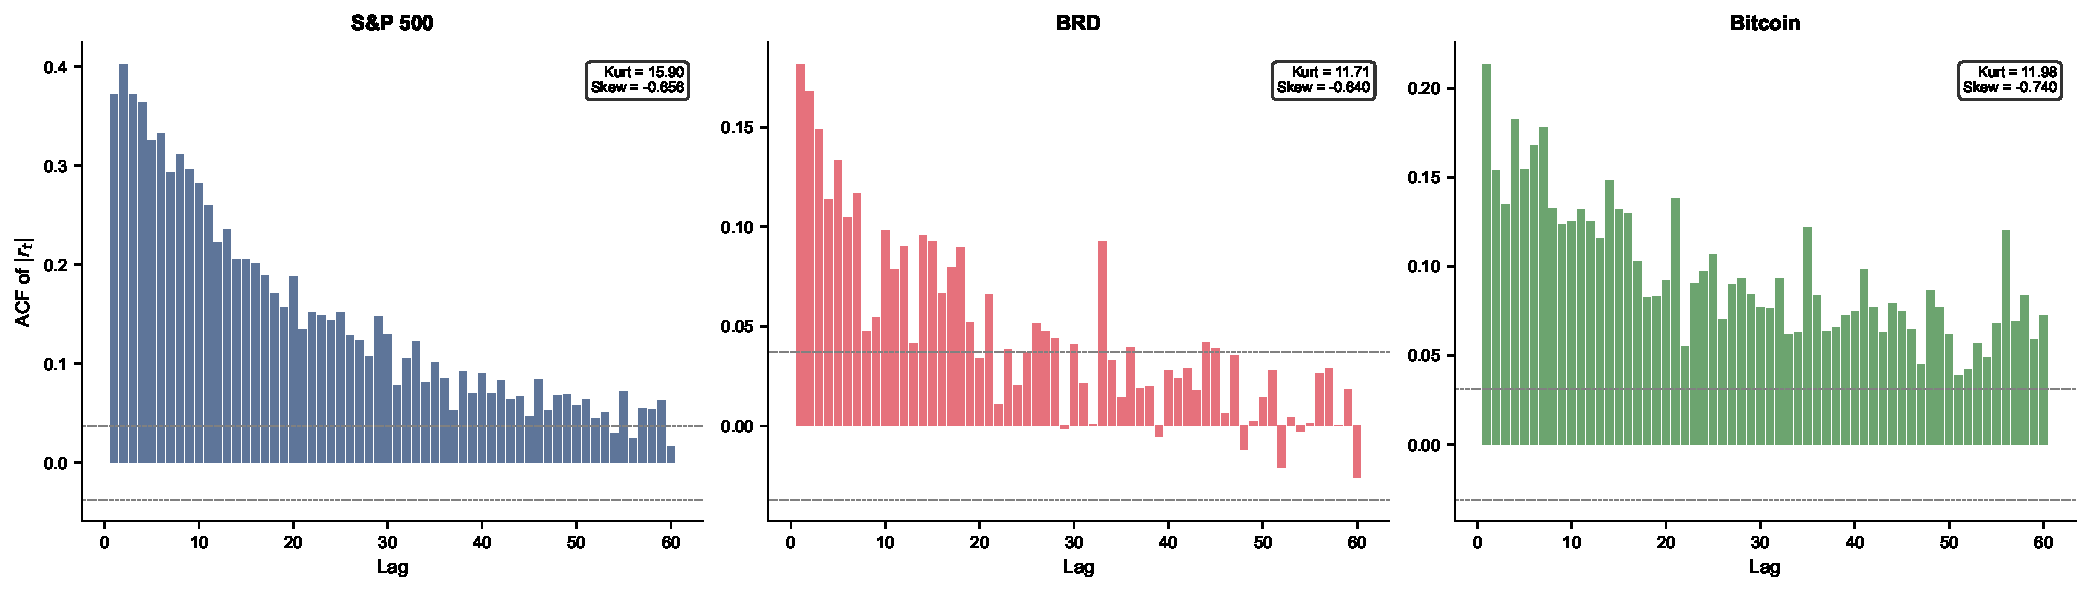
\includegraphics[width=0.78\textwidth]{../../charts/ch2_cs2a_stylized_3assets.pdf}
\end{center}
\vspace{-0.3cm}
\quantlet{SFM\_ch2\_case\_study\_2a}{https://github.com/QuantLet/Stat_fin_markets/tree/master/Ch_02/SFM_ch2_case_study_2a}
\end{frame}

%--- Y3 Slide 3: Normal vs Student-t ---
\begin{frame}{Case Study: Normal vs Student-$t$}
\quantlet{SFM\_ch2\_case\_study\_2a}{https://github.com/QuantLet/Stat_fin_markets/tree/master/Ch_02/SFM_ch2_case_study_2a}
\begin{block}{Log-scale histogram with overlay}
\begin{itemize}\setlength\itemsep{2pt}
\item We compare the two models on a logarithmic scale
\item \textcolor{MainBlue}{Normal} systematically underestimates the tails
\item \textcolor{IDAred}{Student-$t$} adapts well with estimated $\nu$:
\begin{itemize}\setlength\itemsep{1pt}
    \item S\&P 500: $\hat{\nu} \approx 4$--$5$; \quad BRD: $\hat{\nu} \approx 3$--$5$; \quad Bitcoin: $\hat{\nu} \approx 3$--$4$
\end{itemize}
\item The difference grows exponentially in the tails
\end{itemize}
\end{block}
\begin{alertblock}{Implication}
\begin{itemize}
\item On a logarithmic scale, the Normal underestimation becomes visible: empirical tails are orders of magnitude heavier
\end{itemize}
\end{alertblock}
\end{frame}

%--- Y3 Slide 3b: Chart full ---
\begin{frame}{Case Study: Normal vs Student-$t$ --- Chart}
\begin{center}
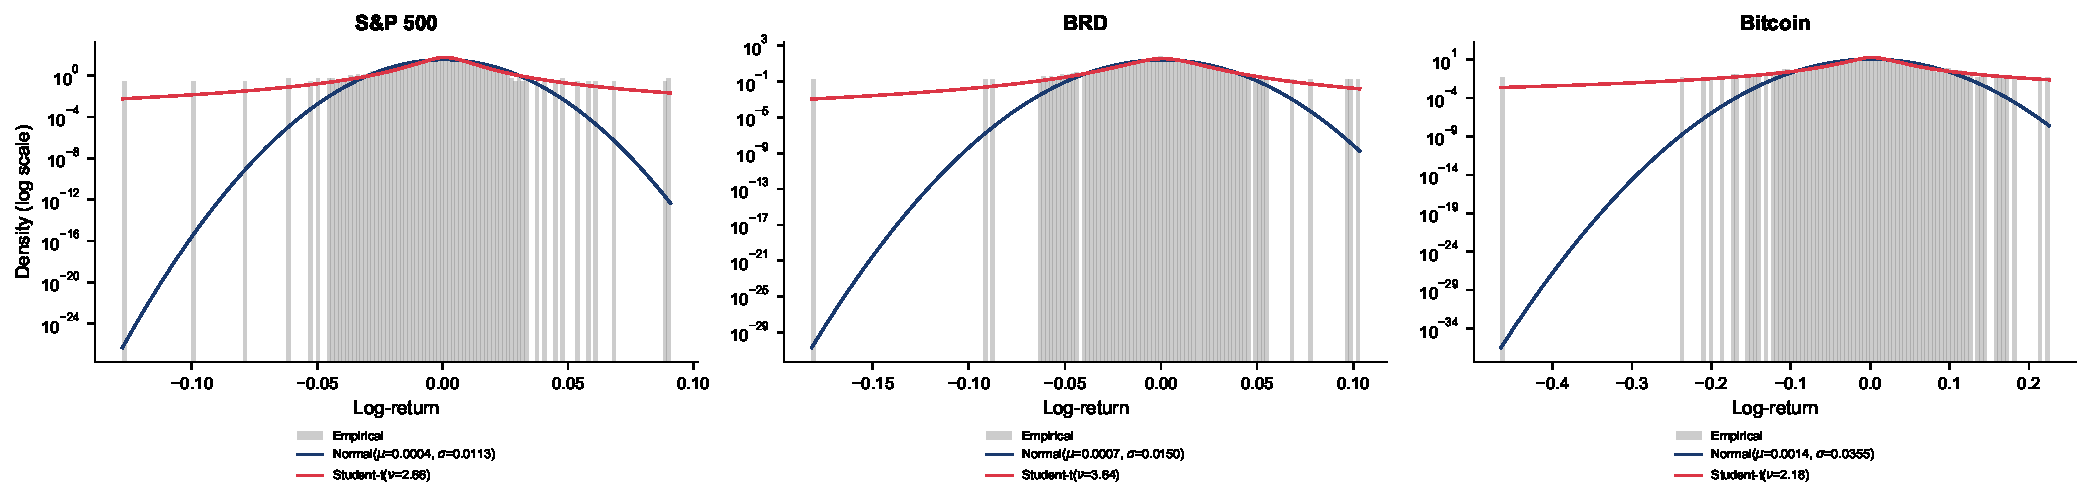
\includegraphics[width=0.82\textwidth]{../../charts/ch2_cs2a_fit_comparison.pdf}
\end{center}
\vspace{-0.3cm}
\quantlet{SFM\_ch2\_case\_study\_2a}{https://github.com/QuantLet/Stat_fin_markets/tree/master/Ch_02/SFM_ch2_case_study_2a}
\end{frame}

%--- Y3 Slide 4: QQ-plots ---
\begin{frame}{Case Study: QQ-Plots}
\vspace{-0.2cm}
    \begin{center}
        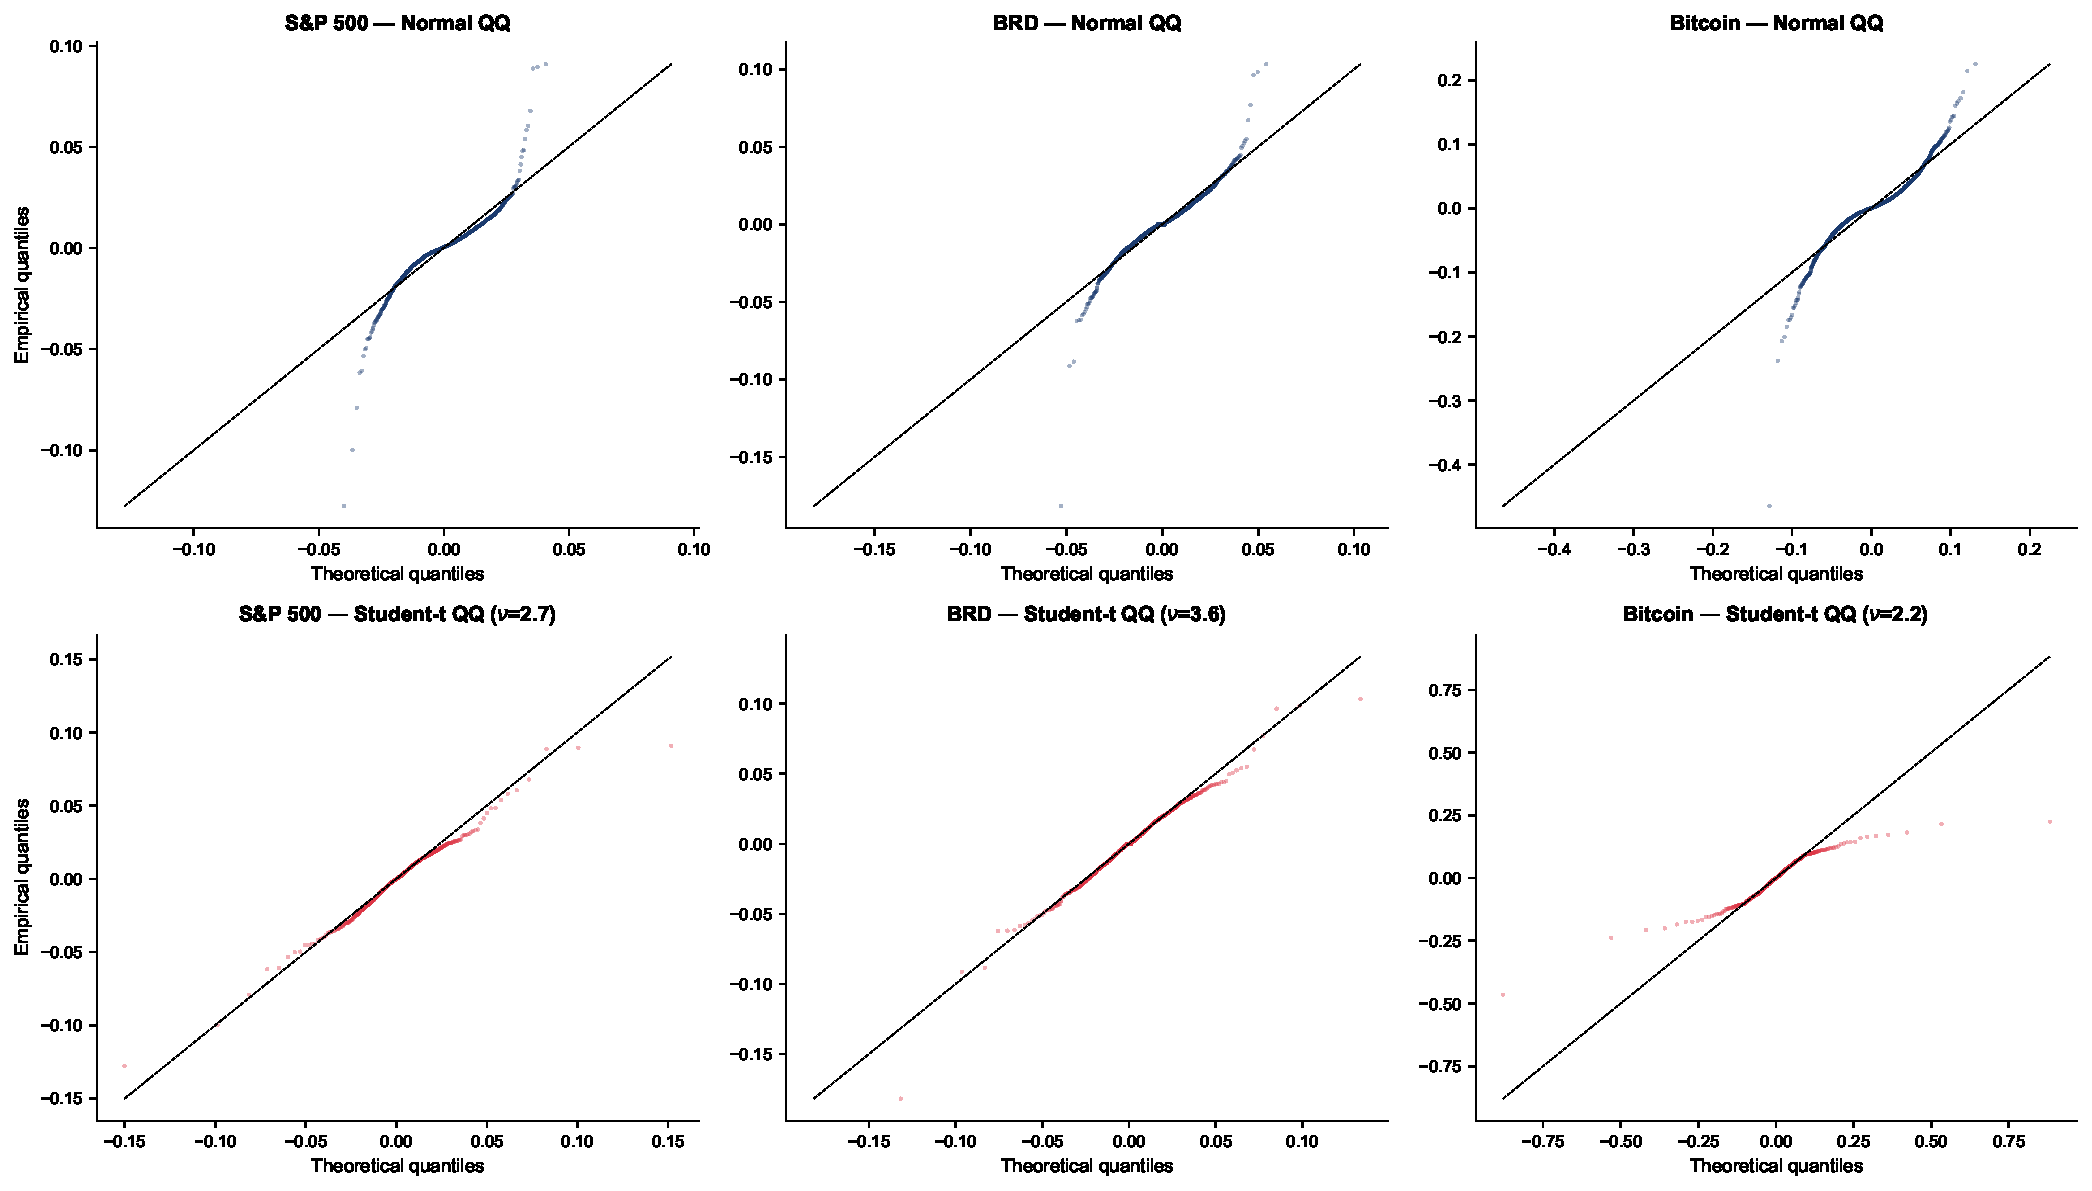
\includegraphics[width=0.60\textwidth]{../../charts/ch2_cs2a_qq_comparison.pdf}
    \end{center}
    \vspace{-0.3cm}
    \quantlet{SFM\_ch2\_case\_study\_2a}{https://github.com/QuantLet/Stat_fin_markets/tree/master/Ch_02/SFM_ch2_case_study_2a}
    \vspace{-0.1cm}
    {\footnotesize
    \begin{itemize}\setlength{\itemsep}{0pt}
        \item \textbf{Normal QQ}: systematic deviations in tails \quad \textbf{Student-$t$ QQ}: much better alignment
        \item Bitcoin: largest deviations, confirming heavier tails
    \end{itemize}}
\end{frame}

%--- Y3 Slide 5: Normality tests ---
\begin{frame}{Case Study: Normality Tests}
    \begin{block}{Testing $H_0$: returns $\sim \mathcal{N}(\mu, \sigma^2)$}
    \small
    {\centering
    \begin{tabular}{lrrrr}
    \toprule
    \textbf{Asset} & \textbf{Jarque--Bera} & \textbf{Shapiro--Wilk} & \textbf{Anderson--Darling} & \textbf{Kolmogorov--Smirnov} \\
    \midrule
    S\&P 500 & $> 10\,000^{***}$ & $< 0.99^{***}$ & $> 20^{***}$ & $> 0.05^{***}$ \\
    BRD      & $> 8\,000^{***}$  & $< 0.99^{***}$ & $> 15^{***}$ & $> 0.04^{***}$ \\
    Bitcoin  & $> 5\,000^{***}$  & $< 0.98^{***}$ & $> 30^{***}$ & $> 0.06^{***}$ \\
    \bottomrule
    \end{tabular}\par}
    \vspace{0.2cm}
    \begin{itemize}
    \item $^{***}$ rejection at level $\alpha = 0.001$ for all tests and all assets
    \end{itemize}
    \end{block}

    \begin{alertblock}{Conclusion}
        \begin{itemize}
            \item Normality is \textbf{decisively rejected} across all three markets
            \item All four tests converge: JB (moments), SW (order), AD (tails), KS (full distribution)
        \end{itemize}
    \end{alertblock}
\end{frame}

%--- Y3 Slide 5b: VaR/ES ---
\begin{frame}{Case Study: VaR and ES --- Normal vs Student-$t$}
    \begin{block}{Applying risk formulas (portfolio 1M EUR, $\mu \approx 0$)}
    \small
    \begin{itemize}\setlength{\itemsep}{0pt}
    \item $\text{VaR}^{N}_{1\%} = 2.326\,\sigma$; \quad $\text{VaR}^{t}_{1\%} = \sqrt{\tfrac{\nu-2}{\nu}}\,|t_\nu^{-1}(0.01)|\,\sigma$; \quad ES: left-tail mean below $\text{VaR}$
    \end{itemize}
    \vspace{0.1cm}

    {\centering
    \renewcommand{\arraystretch}{1.05}
    \footnotesize
    \begin{tabular}{lrrrr}
    \toprule
    \textbf{Asset} ($\sigma$, $\hat{\nu}$) & \textbf{VaR Normal} & \textbf{VaR Student-$t$} & \textbf{ES Normal} & \textbf{ES Student-$t$} \\
    \midrule
    S\&P 500 ($1.15\%$, $4.5$) & 26\,750 & 30\,400 & 30\,500 & 40\,200 \\
    BRD ($1.10\%$, $3.8$)       & 25\,590 & 29\,600 & 29\,300 & 40\,200 \\
    Bitcoin ($3.80\%$, $3.2$)    & 88\,390 & 102\,000 & 100\,900 & 148\,700 \\
    \bottomrule
    \end{tabular}\par}
    \end{block}

    \begin{alertblock}{Normal ES underestimates by 30--50\%}
    \begin{itemize}
        \item $P(r < -3\sigma)$: Normal $= \Phi(-3) = 0.135\%$ (1 day/741); \quad Student-$t$ ($\hat{\nu}\!=\!4.5$) $\approx 0.58\%$ (1 day/172) --- $\mathbf{4.3\times}$ more frequent
    \end{itemize}
    \end{alertblock}
\end{frame}

%--- Y3 Slide 5c: AIC/BIC ---
\begin{frame}{Case Study: Model Selection --- AIC/BIC}
    \begin{block}{Information criteria ($\text{AIC} = -2\ell + 2k$; \; $\text{BIC} = -2\ell + k\ln n$)}
    \small
    {\centering
    \renewcommand{\arraystretch}{1.1}
    \begin{tabular}{lccc}
    \toprule
    \textbf{Asset} & \textbf{$\Delta$AIC (Normal $-$ Student-$t$)} & \textbf{$\Delta$BIC} & \textbf{Winner} \\
    \midrule
    S\&P 500 & $> 200$ & $> 190$ & Student-$t$ \\
    BRD      & $> 150$ & $> 140$ & Student-$t$ \\
    Bitcoin  & $> 300$ & $> 290$ & Student-$t$ \\
    \bottomrule
    \end{tabular}\par}
    \end{block}

    \begin{rmk}
    \begin{itemize}
    \item $\Delta\text{AIC} > 10$ $\Rightarrow$ strong evidence against the Normal model (Burnham \& Anderson)
    \item Student-$t$ wins decisively across all markets, despite having one extra parameter ($\nu$)
    \end{itemize}
    \end{rmk}
\end{frame}

%--- Y3 Slide 6: Conclusions ---
\begin{frame}{Case Study: Conclusions}
    \begin{block}{Lessons from real data analysis}
    \small
    \begin{enumerate}
        \item \textbf{Kurtosis} $\gg 3$ across all markets $\Rightarrow$ the Normal model is inadequate
        \item \textbf{Student-$t$} provides a first approximation, but has \emph{symmetric tails}
        \item \textbf{Skewness} (especially for S\&P 500 and BRD) requires asymmetric models
        \item \textbf{Volatility clustering} demands conditional models (GARCH)
    \end{enumerate}
    \end{block}

    \begin{alertblock}{Risk management implications}
    \begin{itemize}\setlength{\itemsep}{0pt}
        \item Normal ES at 1\% underestimates the mean tail loss by \textbf{30--50\%} compared to Student-$t$
        \item Normal VaR underestimates by $\sim$15\%, but $3\sigma$ events occur $4\times$ more often
    \end{itemize}
    \end{alertblock}
\end{frame}

%--- AI Exercise ---
\begin{frame}[shrink=3]{AI Exercise: Distributions and Tail Risk}
    \begin{cminipage}{0.95\textwidth}
    \begin{block}{\footnotesize Prompt to test in ChatGPT / Claude / Copilot}
        {\small
        ``Download daily data for S\&P~500 and Bitcoin from 2015 to 2025 using Python (\texttt{yfinance}).
        Compute log-returns. Fit a Normal and a Student-$t$ distribution via MLE on each series.
        Compare models using AIC/BIC, QQ-plot, and log-scale histogram.
        Compute 1\% VaR and Expected Shortfall under both models.
        Estimate the Pareto tail index using the Hill estimator.''}
    \end{block}
    \vspace{-1mm}
    {\small
    \textbf{Exercise}:
    \begin{enumerate}
        \item Does the AI compute log-returns correctly? Check: $r_t = \ln(P_t / P_{t-1})$, not $(P_t - P_{t-1})/P_{t-1}$
        \item Are the estimated degrees of freedom $\hat{\nu}$ plausible ($\hat{\nu} \in [3, 8]$ for daily data)?
        \item Are the VaR and ES formulas correct? Check: $\text{VaR}^{t}_{1\%}$ uses adjusted scale $s = \sigma\sqrt{(\nu-2)/\nu}$?
        \item Ask the AI: ``What happens to VaR if $\nu \leq 2$?'' Does it mention infinite variance?
        \item Does the Hill plot show a stable region? What value of $\hat{\alpha}$ does it obtain? Compare with $\hat{\nu}$ from Student-$t$
    \end{enumerate}
    }
    \vspace{-1mm}
    \begin{alertblock}{}
        {\small
        \begin{itemize}\setlength{\itemsep}{0pt}
            \item \textbf{Warning}: AI often confuses \textit{excess kurtosis} ($\kappa - 3$) with total kurtosis ($\kappa$). Always verify the definition used.
        \end{itemize}
        }
    \end{alertblock}
    \end{cminipage}
\end{frame}

%#############################################################################
\section{Quiz}
%#############################################################################

\begin{frame}{Question 1}
    \begin{cminipage}{0.95\textwidth}
    \begin{alertblock}{Question}
        \begin{itemize}
            \item The event of October 19, 1987 (S\&P~500 $-20.5\%$) corresponds to a $\sim$20$\sigma$ event under the Normal assumption ($\sigma \approx 1\%$). What is the probability of such an event?
        \end{itemize}
    \end{alertblock}

    \vspace{0.3cm}

    \begin{block}{Answer choices}
        \begin{itemize}\setlength{\itemsep}{2pt}
        \item \textcolor{MainBlue}{\textbf{(A)}} $\approx 10^{-2}$ (1 in 100)
        \item \textcolor{MainBlue}{\textbf{(B)}} $\approx 10^{-30}$ (practically impossible on a human timescale)
        \item \textcolor{MainBlue}{\textbf{(C)}} $\approx 10^{-89}$ (impossible in the lifetime of the universe)
        \item \textcolor{MainBlue}{\textbf{(D)}} $\approx 10^{-6}$ (once every million days)
        \end{itemize}
    \end{block}
    \end{cminipage}
\end{frame}

\begin{frame}{Question 1: Answer}
    \begin{cminipage}{0.95\textwidth}
    \begin{exampleblock}{Answer: (C)}
    \begin{itemize}\setlength\itemsep{1pt}
        \item \textbf{Normal}: $\sigma \approx 1\%$, so $-20.5\%$ $= 20.5\sigma$. $P = 2\Phi(-20.5) \approx 10^{-89}$.
        \item \textbf{Student-$t$ ($\nu = 5$)}: adjusted scale $s = \sigma\sqrt{3/5} = 0.775\%$; $t_{\text{stat}} = 20.5/0.775 = 26.5$; $P(|T_5| > 26.5) \approx 10^{-8}$ --- still extreme, but \textbf{$10^{81}\times$ more probable} than under Normal!
        \item Yet it happened --- demonstrating the \textbf{inadequacy of the Normal distribution}.
        \item Under stable distributions ($\alpha \approx 1.7$), the probability rises to $\sim 10^{-3}$.
    \end{itemize}
    \end{exampleblock}
    \end{cminipage}
\end{frame}

\begin{frame}{Question 2}
    \begin{cminipage}{0.95\textwidth}
    \begin{alertblock}{Question}
        \begin{itemize}
            \item A Student-$t$ distribution with $\nu = 4$ degrees of freedom has:
        \end{itemize}
    \end{alertblock}

    \vspace{0.3cm}

    \begin{block}{Answer choices}
        \begin{itemize}\setlength{\itemsep}{2pt}
        \item \textcolor{MainBlue}{\textbf{(A)}} Finite mean, finite variance, finite kurtosis
        \item \textcolor{MainBlue}{\textbf{(B)}} Finite mean, finite variance, infinite kurtosis
        \item \textcolor{MainBlue}{\textbf{(C)}} Finite mean, infinite variance, infinite kurtosis
        \item \textcolor{MainBlue}{\textbf{(D)}} Infinite mean, infinite variance, infinite kurtosis
        \end{itemize}
    \end{block}
    \end{cminipage}
\end{frame}

\begin{frame}{Question 2: Answer}
    \begin{cminipage}{0.95\textwidth}
    \begin{exampleblock}{Answer: (B)}
    \begin{itemize}
        \item For Student-$t$: mean exists if $\nu > 1$, variance if $\nu > 2$, kurtosis if $\nu > 4$.
        \item With $\nu = 4$: finite mean (\checkmark), finite variance ($= \nu/(\nu-2) = 2$, \checkmark), but kurtosis \textbf{does not exist} (4th moment diverges: $6/(\nu-4)$ with $\nu=4$).
        \item (A) is wrong: the 4th moment does not exist at $\nu = 4$ exactly.
        \item This shows that even distributions with finite variance can have \textbf{very heavy} tails.
    \end{itemize}
    \end{exampleblock}
    \end{cminipage}
\end{frame}

\begin{frame}{Question 3: Reasoning --- Basel III and Distribution Choice}
    \begin{cminipage}{0.95\textwidth}
    \begin{alertblock}{Question}
        \begin{itemize}
            \item A bank computes regulatory capital using ES at 2.5\% under the Normal distribution. Supervisors discover that portfolio returns have $\hat{\nu} = 4$ (Student-$t$). What is the consequence?
        \end{itemize}
    \end{alertblock}

    \vspace{0.3cm}

    \begin{block}{Answer choices}
        \begin{itemize}\setlength{\itemsep}{2pt}
        \item \textcolor{MainBlue}{\textbf{(A)}} Capital is sufficient --- ES does not depend on the distribution shape
        \item \textcolor{MainBlue}{\textbf{(B)}} Capital is underestimated by 30--50\%, the bank must increase reserves
        \item \textcolor{MainBlue}{\textbf{(C)}} Capital is overestimated --- Student-$t$ predicts lower risks
        \item \textcolor{MainBlue}{\textbf{(D)}} Cannot decide without knowing the volatility
        \end{itemize}
    \end{block}
    \end{cminipage}
\end{frame}

\begin{frame}{Question 3: Answer}
    \begin{cminipage}{0.95\textwidth}
    \begin{exampleblock}{Answer: (B)}
    \begin{itemize}
        \item Student-$t$ with $\nu = 4$ has much heavier tails than Normal: $P(r < -3\sigma)$ is $\sim$4$\times$ larger.
        \item ES under Student-$t$ is \textbf{30--50\% larger} than under Normal (as demonstrated in the case study).
        \item (A) is wrong: ES depends critically on the shape of the tails, not just on $\sigma$.
        \item (D) is wrong: even with the same $\sigma$, Student-$t$ gives larger ES due to heavier tails.
        \item \textbf{Lesson}: Distribution choice is not academic --- it \textbf{directly determines bank capital}.
    \end{itemize}
    \end{exampleblock}
    \end{cminipage}
\end{frame}

%#############################################################################
\section{Exam Exercises}
%#############################################################################

\begin{frame}{Exercise 1: Log-Returns and Moments}
\begin{block}{Problem}
\begin{itemize}
\item Given daily closing prices:
\end{itemize}
\begin{center}
{\small
\renewcommand{\arraystretch}{1.2}
\begin{tabular}{lccccc}
\toprule
$t$ & 0 & 1 & 2 & 3 & 4 \\
\midrule
$P_t$ & 100 & 103 & 98 & 95 & 102 \\
\bottomrule
\end{tabular}
}
\end{center}
\end{block}
\begin{enumerate}
    \item Compute log-returns $r_t = \ln(P_t/P_{t-1})$ for $t = 1, \ldots, 4$.
    \item Compute sample mean, variance, skewness, and kurtosis.
    \item Apply the Jarque--Bera test: $JB = \frac{n}{6}\left(S^2 + \frac{(K-3)^2}{4}\right)$. Is normality rejected at 5\%?
    \item Compute the total log-return over 4 periods. Verify time-additivity.
\end{enumerate}
\end{frame}

\begin{frame}{Exercise 2: The Normal Distribution and VaR}
\begin{block}{Problem}
\begin{itemize}
\item A \$5M portfolio has daily returns $\sim N(\mu, \sigma^2)$ with $\hat{\mu} = 0.04\%$ and $\hat{\sigma} = 1.2\%$
\end{itemize}
\end{block}
\begin{enumerate}
    \item Compute daily VaR at levels 5\%, 1\%, and 0.1\%.
    \item Compute Expected Shortfall at the 1\% level.
    \item A $-4\%$ event occurred. What is its probability under the Normal assumption?
    \item Argue why Normal VaR may underestimate real risk.
\end{enumerate}
\vspace{0.1cm}
\begin{exampleblock}{Hint}
$\text{VaR}_\alpha = -(\mu + z_\alpha \cdot \sigma)$, where $z_{0.05} = -1.645$, $z_{0.01} = -2.326$, $z_{0.001} = -3.090$.
\end{exampleblock}
\end{frame}

\begin{frame}{Exercise 3: Student-$t$ --- Fitting and Comparison}
\begin{block}{Problem}
\begin{itemize}
\item Using the data from Exercise 1, suppose MLE produces: Normal $\ell = 12.5$, Student-$t$ ($\nu = 5$) $\ell = 14.8$
\end{itemize}
\end{block}
\begin{enumerate}
    \item Compute AIC and BIC for both models ($k_N = 2$, $k_t = 3$, $n = 4$).
    \item Which model is preferred by AIC? By BIC?
    \item Compute the excess kurtosis of the Student-$t$ distribution with $\nu = 5$.
    \item Explain why Student-$t$ captures heavy tails better than the Normal distribution.
\end{enumerate}
\vspace{0.1cm}
\begin{alertblock}{Formulas}
\begin{itemize}
\item $\text{AIC} = -2\ell + 2k$, \quad $\text{BIC} = -2\ell + k\ln n$, \quad $\kappa = 6/(\nu - 4)$ for $\nu > 4$
\end{itemize}
\end{alertblock}
\end{frame}

\begin{frame}{Exercise 4: Comparing VaR/ES --- Normal, Student-$t$, Pareto}
\begin{block}{Problem}
\begin{itemize}
\item A \$10M portfolio has daily returns with $\hat{\sigma} = 1.5\%$, $\mu \approx 0$. The Hill estimator on the left tail gives $\hat{\alpha} = 3.5$
\end{itemize}
\end{block}
\begin{enumerate}
    \item Compute 1\% VaR under: (a) Normal; (b) Student-$t$ with $\nu = 5$; (c) Pareto with $\alpha = 3.5$, $x_m = 0.01$
    \item Compute 1\% ES under each model. \textit{Hint}: $\text{ES}^{\text{Pareto}}_\alpha = \frac{\alpha}{\alpha - 1}\,\text{VaR}_\alpha$ for $\alpha > 1$
    \item Fill in the table and discuss the differences:
\end{enumerate}
\vspace{0.1cm}
{\small
\begin{center}
\begin{tabular}{lccc}
\toprule
& \textbf{Normal} & \textbf{Student-$t$ ($\nu\!=\!5$)} & \textbf{Pareto ($\alpha\!=\!3.5$)} \\
\midrule
VaR 1\% & ? & ? & ? \\
ES 1\%  & ? & ? & ? \\
ES/VaR  & ? & ? & ? \\
\bottomrule
\end{tabular}
\end{center}
}
\end{frame}

%--- Python Lab ---
\begin{frame}{Python Lab --- Interactive Exercises}
\small
\begin{block}{Lab 1: Distribution Fitting (Y3)}
\begin{enumerate}
\item Open \texttt{SFM\_ch2\_normal\_distribution.ipynb}
\item Download S\&P~500 data (2015--2025); compute log-returns
\item Histogram + Normal overlay; Jarque--Bera test
\item Fit Student-$t$ (MLE). Compare AIC with Normal model
\end{enumerate}
\end{block}
\quantlet{SFM\_ch2\_normal\_distribution}{https://github.com/QuantLet/Stat_fin_markets/tree/master/Ch_02/SFM_ch2_normal_distribution}
\end{frame}

%#############################################################################
\section*{Exercise Solutions}
%#############################################################################

\begin{frame}{Exercise 1: Solution}
\begin{block}{Solution}
\begin{enumerate}
\item Log-returns: $r_1 = \ln(103/100) = 0.0296$, $r_2 = \ln(98/103) = -0.0498$, $r_3 = \ln(95/98) = -0.0311$, $r_4 = \ln(102/95) = 0.0713$
\item $\bar{r} = (0.0296 - 0.0498 - 0.0311 + 0.0713)/4 = 0.0050$; \;$s^2 = \frac{1}{3}\sum(r_i - \bar{r})^2 = 0.00253$; \;$s = 0.0503$. Skewness: $S \approx 0.56$; \;Kurtosis: $K \approx 1.72$
\item $JB = \frac{4}{6}(0.56^2 + (1.72-3)^2/4) = 0.48$. With $\chi^2_2(0.05) = 5.99$: $0.48 < 5.99$ $\Rightarrow$ \textbf{do not reject} normality (sample too small!)
\item $r_{0:4} = \ln(102/100) = 0.0198 = r_1 + r_2 + r_3 + r_4 = 0.0198$ \checkmark
\end{enumerate}
\end{block}
\end{frame}

\begin{frame}{Exercise 2: Solution}
\begin{block}{Solution}
\begin{enumerate}
\item $\text{VaR}_\alpha = -(\mu + z_\alpha\sigma) \times W$, with $\mu = 0.0004$, $\sigma = 0.012$, $W = \$5$M:
\begin{itemize}
\item VaR 5\%: $0.01934 \times 5\text{M} = \$96,680$; \; VaR 1\%: $\$137,560$; \; VaR 0.1\%: $\$183,400$
\end{itemize}
\item $\text{ES}_{1\%} = \sigma \cdot \phi(-2.326)/0.01 = 0.03198$ $\Rightarrow$ \$159,900
\item $P(r < -0.04) = \Phi(-3.37) \approx 0.038\%$ (1 day in $\sim$2,600)
\item Empirically, events $> 3\sigma$ occur much more frequently $\Rightarrow$ Normal VaR underestimates risk
\end{enumerate}
\end{block}
\end{frame}

\begin{frame}{Exercise 3: Solution}
\begin{block}{Solution}
\begin{enumerate}
\item With $\ell_N = 12.5$, $\ell_t = 14.8$, $k_N = 2$, $k_t = 3$, $n = 4$:
\begin{itemize}
\item Normal: AIC $= -21.0$; BIC $= -22.23$. \; Student-$t$: AIC $= -23.6$; BIC $= -25.44$
\end{itemize}
\item Student-$t$ wins on both criteria (AIC: $-23.6 < -21.0$; BIC: $-25.44 < -22.23$)
\item Excess kurtosis: $\kappa = 6/(\nu - 4) = 6/(5-4) = 6$. Total kurtosis: $3 + 6 = 9$
\item The Student-$t$ PDF decays as $|x|^{-(\nu+1)}$ (power law) vs.\ $e^{-x^2/2}$ for Normal. The slower decay allocates more probability to the tails
\end{enumerate}
\end{block}
\end{frame}

%#############################################################################
\section{Conclusions}
%#############################################################################

%--- Y3 Slide 1 ---
\begin{frame}{Key Takeaways}
\begin{enumerate}
\item Financial returns are \textbf{not Normal}: fat tails, skewness, volatility clustering
\item \textbf{Student-$t$}: simplest heavy-tailed model, captures excess kurtosis
\item \textbf{Stable distributions}: theoretically motivated (GCLT), infinite variance possible
\item \textbf{EVT}: rigorous framework for extreme tail modeling
\item \textbf{VaR and ES}: the distribution choice directly affects risk measurement
\begin{itemize}
\item 1\% VaR under Normal $\ll$ 1\% VaR under Student-$t$ $\ll$ 1\% VaR under Stable
\end{itemize}
\item \textbf{No single best model}: choice depends on application (pricing, risk, regulation)
\end{enumerate}

\vspace{0.2cm}
\begin{block}{Central Message}
\begin{itemize}
\item \textbf{Underestimating tail risk has real consequences}: insufficient capital, unexpected losses, and systemic crises
\item Accurate distributional modeling is not an academic exercise --- it is a regulatory and financial necessity
\end{itemize}
\end{block}
\end{frame}

%--- Y3 Slide 2 ---
\begin{frame}{Homework Assignments}
\textbf{Year 3}:
\begin{enumerate}
\item Download 5 years of daily prices for a stock. Compute log-returns, sample moments, and test normality (Jarque--Bera).
\item Fit Normal and Student-$t$ distributions via MLE. Compare using AIC/BIC and QQ-plots.
\item Compute 1\% VaR and 0.1\% VaR under both models for a \$1M portfolio.
\end{enumerate}

\vspace{0.2cm}
\textbf{additional}:
\begin{enumerate}\setcounter{enumi}{3}
\item Fit Hansen's skewed-$t$ and compute ES at the 1\% level.
\item Perform a rolling-window VaR backtest (250-day window) and apply the Kupiec test.
\end{enumerate}
\end{frame}

%--- MSc Slide 3 ---
\begin{frame}{Advanced Homework}
\begin{enumerate}\setcounter{enumi}{5}
\item Fit a stable distribution to your data using MLE. Report $(\hat{\alpha}, \hat{\beta}, \hat{\gamma}, \hat{\delta})$.
\item Apply the POT method: select threshold, fit GPD, compute EVT-based 1\% VaR and ES.
\item Compare all models (Normal, Student-$t$, skewed-$t$, Stable, EVT) in a summary table.
\end{enumerate}

\vspace{0.3cm}
\textbf{additional}:
\begin{enumerate}\setcounter{enumi}{8}
\item Implement the Hill estimator. Create a Hill plot and discuss the bias--variance trade-off.
\item Fit a GARCH(1,1)-$t$ model. Compare the distribution of standardized residuals with the unconditional return distribution.
\end{enumerate}
\end{frame}

%--- PhD Slide 4 ---
\begin{frame}{Research Directions}
\begin{itemize}
\item \textbf{Open questions}:
\begin{itemize}
\item Is the true tail index of financial returns closer to $\alpha \approx 3$ (finite variance) or $\alpha \approx 1.7$ (infinite variance)?
\item How should we aggregate risk when distributions have infinite variance?
\item Can machine learning improve distributional forecasting?
\end{itemize}
\item \textbf{Suggested readings}:
\begin{itemize}
\item Cont (2001): ``Empirical properties of asset returns: stylized facts and statistical issues''
\item McNeil, Frey \& Embrechts (2015): \textit{Quantitative Risk Management}
\item Nolan (2020): \textit{Stable Distributions --- Models for Heavy Tailed Data}
\item Rachev (2003): \textit{Handbook of Heavy Tailed Distributions in Finance}
\end{itemize}
\end{itemize}
\end{frame}

%#############################################################################
\section*{References}
%#############################################################################

\begin{frame}{References I}
\small
\begin{thebibliography}{99}
\bibitem{mandelbrot63} Mandelbrot, B. (1963). The variation of certain speculative prices. \textit{Journal of Business}, 36(4), 394--419.
\bibitem{fama65} Fama, E. (1965). The behavior of stock-market prices. \textit{Journal of Business}, 38(1), 34--105.
\bibitem{cont01} Cont, R. (2001). Empirical properties of asset returns: stylized facts and statistical issues. \textit{Quantitative Finance}, 1(2), 223--236.
\bibitem{hansen94} Hansen, B. (1994). Autoregressive conditional density estimation. \textit{International Economic Review}, 35(3), 705--730.
\bibitem{nolan97} Nolan, J. P. (1997). Numerical calculation of stable densities and distribution functions. \textit{Stochastic Models}, 13(4), 759--774.
\bibitem{mcneil05} McNeil, A., Frey, R. \& Embrechts, P. (2015). \textit{Quantitative Risk Management}. Princeton University Press.
\bibitem{bn77} Barndorff-Nielsen, O. (1977). Exponentially decreasing distributions for the logarithm of particle size. \textit{Proceedings of the Royal Society of London A}, 353, 401--419.
\end{thebibliography}
\end{frame}

\begin{frame}{References II}
\small
\begin{thebibliography}{99}
\bibitem{hamilton89} Hamilton, J. D. (1989). A new approach to the economic analysis of nonstationary time series. \textit{Econometrica}, 57(2), 357--384.
\bibitem{merton76} Merton, R. (1976). Option pricing when underlying stock returns are discontinuous. \textit{Journal of Financial Economics}, 3, 125--144.
\bibitem{rachev03} Rachev, S. T. (2003). \textit{Handbook of Heavy Tailed Distributions in Finance}. Elsevier.
\bibitem{nolan20} Nolan, J. P. (2020). \textit{Stable Distributions --- Models for Heavy Tailed Data}. Birkh\"{a}user.
\bibitem{vuong89} Vuong, Q. H. (1989). Likelihood ratio tests for model selection and non-nested hypotheses. \textit{Econometrica}, 57(2), 307--333.
\bibitem{fissler16} Fissler, T. \& Ziegel, J. F. (2016). Higher order elicitability and Osband's principle. \textit{Annals of Statistics}, 44(4), 1680--1707.
\bibitem{bns01} Barndorff-Nielsen, O. \& Shephard, N. (2001). Non-Gaussian Ornstein--Uhlenbeck-based models. \textit{Journal of the Royal Statistical Society B}, 63(2), 167--241.
\end{thebibliography}
\end{frame}

\end{document}
